%
% @author  unknown
% @version 1.1a
% @edit by Andreas Febrian
% @edit by Moeljono Widjaja
% @edit by Arya Wicaksana
%
% Template Laporan Skripsi Informatika UMN
%

%
% Tipe dokumen adalah report dengan satu kolom. 
%
\documentclass[12pt, a4paper, onecolumn, oneside, final]{report1}

% \usepackage{indentfirst}

% Load konfigurasi LaTeX untuk tipe laporan thesis
\usepackage{_internals/umnthesis}

% Daftar pemenggalan suku kata dan istilah dalam LaTeX
%
% Hyphenation untuk Indonesia 
%
% @author  Andreas Febrian
% @version 1.00
% 
% Tambahkan cara pemenggalan kata-kata yang salah dipenggal secara otomatis 
% oleh LaTeX. Jika kata tersebut dapat dipenggal dengan benar, maka tidak 
% perlu ditambahkan dalam berkas ini. Tanda pemenggalan kata menggunakan 
% tanda '-'; contoh:
% menarik
%   --> pemenggalan: me-na-rik
%

\hyphenation{
    % alphabhet A
    a-na-li-sa a-tur 
    a-pli-ka-si 
    % alphabhet B
    ba-ngun-an 
    be-be-ra-pa 
    ber-ge-rak
    ber-ke-lan-jut-an 
    ber-pe-nga-ruh 
    % alphabhet C
    ca-ri
    % alphabhet D
    di-sim-pan di-pim-pin de-ngan da-e-rah di-ba-ngun da-pat di-nya-ta-kan 
    di-sim-bol-kan di-pi-lih di-li-hat de-fi-ni-si
    % alphabhet E
    e-ner-gi eks-klu-sif
    % alphabhet F
    fa-si-li-tas
    % alphabhet G
    ga-bung-an ge-rak
    % alphabhet H
    ha-lang-an
    % alphabhet I
    % alphabhet J
    % alphabhet K
    ke-hi-lang-an
    ku-ning 
    kua-li-tas ka-me-ra ke-mung-kin-an ke-se-pa-ham-an
    % alphabhet L
    ling-kung-an
    % alphabhet M
    me-neng-ah
    meng-a-tas-i me-mung-kin-kan me-nge-na-i me-ngi-rim-kan 
    meng-u-bah meng-a-dap-ta-si me-nya-ta-kan mo-di-fi-ka-si
    meng-a-tur
    % alphabhet N
    nya-ta non-eks-klu-sif
    % alphabhet O
    % alphabhet P
	pe-nye-rap-an 
	pe-ngon-trol
    pe-mo-del-an
    pe-ran  pe-ran-an-nya
    pem-ba-ngun-an pre-si-den pe-me-rin-tah prio-ri-tas peng-am-bil-an 
    peng-ga-bung-an pe-nga-was-an pe-ngem-bang-an 
    pe-nga-ruh pa-ra-lel-is-me per-hi-tung-an per-ma-sa-lah-an 
    pen-ca-ri-an peng-struk-tur-an
    % alphabhet Q
    % alphabhet R
    ran-cang-an
    % alphabhet S
    si-mu-la-si sa-ngat
    % alphabhet T
    te-ngah
    ter-da-pat
    % alphabhet U
    % alphabhet V
    % alphabhet W
    % alphabhet X
    % alphabhet Y
    % alphabhet Z
    % special
}

% Load konfigurasi khusus untuk laporan yang sedang dibuat
%-----------------------------------------------------------------------------%
% Informasi Mengenai Dokumen
%-----------------------------------------------------------------------------%
% 
% Judul laporan. 
\var{\judul}{Pengembangan Backend Sistem Informasi Kepegawaian CHRIS pada PT Ganda Visi Jayatama}
% Judul Pendek (Tiga Kata Pertama). 
\var{\judulPendek}{Pengembangan Backend Sistem}
% 
% Tulis kembali judul laporan, kali ini akan diubah menjadi huruf kapital
% \Var{\Judul}{Judul Tugas Akhir}

\Var{\Judul}{Pengembangan Backend Sistem Informasi Kepegawaian CHRIS pada PT Ganda Visi Jayatama}
% 
% Tulis kembali judul laporan namun dengan bahasa Ingris 
\var{\judulInggris}{Backend Enhancement of the CHRIS HR Information System at PT Ganda Visi Jayatama}

% 
% Tipe laporan:
% Laporan MBKM Magang
% Laporan MBKM Kewirausahaan
% Laporan MBKM Penelitian
% Laporan MBKM Proyek Desa
% Laporan MBKM Independent

\var{\type}{Laporan MBKM Magang}
% 
% Tulis kembali tipe laporan, kali ini akan diubah menjadi huruf kapital
\Var{\Type}{Laporan MBKM Magang}
% 
% Tulis nama penulis 
\var{\penulis}{Jose Andreas Lie}
% 
% Tulis kembali nama penulis, kali ini akan diubah menjadi huruf kapital
\Var{\Penulis}{Jose Andreas Lie}

% Informasi tempat kerja magang
\var{\namaPerusahaan}{PT Ganda Visi Jayatama}
\var{\divisi}{Backend Engineer Intern}
\var{\alamatPerusahaan}{Ruko Crystal 1. 19, Jl. Gading Golf Boulevard No.18, Tangerang Regency, Banten 15810}
\var{\periodeMagang}{13 Januari 2025 - 13 Juli 2025}
\var{\pembimbingLapangan}{Pembimbing Lapangan}

% 
% Tulis NIM penulis
\var{\nim}{00000067097}
%
% Tuliskan Jenjang Studi penulis (D3/S1/S2)
\Var{\Jenjang}{S1}
\var{\jenjang}{S1}
% 
% Tuliskan Fakultas dimana penulis berada
\Var{\Fakultas}{Teknik dan Informatika}
\var{\fakultas}{Teknik dan Informatika}
% 
% Tuliskan Program Studi yang diambil penulis
\Var{\Program}{INFORMATIKA}
\var{\program}{Informatika}
% 
% Tuliskan tahun publikasi laporan
\Var{\bulan}{"Bulan"}
\Var{\tahun}{2025}
% 
% Tuliskan gelar yang akan diperoleh dengan menyerahkan laporan ini
\var{\gelar}{Sarjana Ilmu Komputer}
% 
% Tuliskan tanggal pengesahan laporan
\var{\tanggalPengesahan}{Tgl. Pengesahan} 


% Tuliskan tanggal pengumpulan laporan, waktu dimana laporan diserahkan ke 
% penguji/sekretariat
\var{\tanggalPengumpulan}{Tgl. Pengumpulan} 


% Tuliskan tanggal sidang
\var{\hariTanggalSidang}{Senin?, Tgl. Sidang?} 
\var{\waktuSidang}{00.00 s/s 00.00} 

% 
% Tuliskan tanggal keputusan sidang dikeluarkan dan penulis dinyatakan 
% lulus/tidak lulus
\var{\tanggalLulus}{Tgl. Lulus}
% 


% Tuliskan Rektor UMN
\var{\rektorUMN}{ Dr. Ir. Andrey Andoko, M.Sc.}

% Tuliskan Dekan FTI
\var{\dekanFTI}{Dr.   Eng.   Niki  Prastomo,  S.T.,  M.Sc.}

% Tuliskan Kaprodi Informatika 
\var{\kaprodi}{Arya Wicaksana, S.Kom., M.Eng.Sc., OCA}
\var{\kaprodiNIDN}{ NIDN: 0315109103}

% Tuliskan pembimbing tunggal atau ke-1
\var{\pembimbing}{Dr. Ivransa Zuhdi Pane, B.Eng., M.Eng.}
% Tuliskan NIDN pembimbing tunggal atau ke-1
\var{\pembimbingNIDN}{NIDN: 0012345600}

% Tuliskan pembimbing ke-2
\var{\pembimbingb}{Nama Lengkap Beserta Gelar}
% Tuliskan NIDN pembimbing ke-2
\var{\pembimbingbNIDN}{NIDN: 0012345600}

% Tuliskan ketua sidang
\var{\ketuaSidang}{Nama Lengkap Beserta Gelar}

% Tuliskan dosen penguji
\var{\penguji}{Nama Lengkap Beserta Gelar}
\var{\pengujiNIDN}{NIDN: 0123456789}
% 
% Alias untuk memudahkan alur penulisan pada saat menulis laporan
\var{\saya}{Penulis}

%-----------------------------------------------------------------------------%
% Judul Setiap Bab
%-----------------------------------------------------------------------------%
% 
% Berikut ada judul-judul setiap bab. 
% Silahkan diubah sesuai dengan kebutuhan. 
% 
\Var{\kataPengantar}{Kata Pengantar}
\Var{\babSatu}{Pendahuluan}
\Var{\babDua}{Gambaran Umum Perusahaan}
\Var{\babTiga}{Pelaksanaan Kerja Magang}
\Var{\babEmpat}{Simpulan dan Saran}

% Daftar istilah yang mungkin perlu ditandai 
\var{\license}{\f{Creative Common License 1.0 Generic}}
\var{\bslash}{$\setminus$}



% Awal bagian penulisan laporan
\begin{document}
\hyphenpenalty=10000
%
% Sampul Laporan
\onehalfspacing
\NoBgThispage
\begin{titlepage}
    \begin{center}    
    
        % \vspace*{1.0cm}
        % judul thesis harus dalam 14pt Times New Roman


        \begin{minipage}{0.9\textwidth}
            \centering
            \bo{\large  \Judul} 
        \end{minipage}
        
            
        
        


        
        \vspace*{0.5cm}
        \begin{figure}
            \begin{center}
                % \includegraphics[width=2.5cm]{_internals/makara.eps}
                
\includegraphics[width=5cm]{assets/pics/logo_UMN_clean.png}
            \end{center}
        \end{figure}    
        % \vspace*{0.5cm}        % harus dalam 14pt Times New Roman
        \MakeUppercase{ \large \Type }
        \vspace*{5cm}
               
        
        % Diajukan sebagai salah satu syarat untuk memperoleh\\
        % Gelar Sarjana Komputer (S.Kom.) \\[1cm]
        % penulis dan npm
        \MakeUppercase{ \large \bo{\penulis}} \\
        \bo{\large \nim} \\

        \vfill

        % informasi mengenai fakultas dan program studi
        \bo{ \large
        	PROGRAM STUDI \Program \\
        	FAKULTAS \Fakultas\\
        	UNIVERSITAS MULTIMEDIA NUSANTARA\\
        	TANGERANG \\
        	\tahun
        }
    \end{center}
\end{titlepage}


%
% Gunakan penomeran romawi
\pagenumbering{roman}
% setelah bagian ini, halaman dihitung sebagai halaman ke 2
\setcounter{page}{1}

\BgThispage



\pagestyle{fancy}

% Halaman Judul
\addChapter{HALAMAN JUDUL}
\onehalfspacing
    \begin{center}    
    
        % \vspace*{1.0cm}
        % judul thesis harus dalam 14pt Times New Roman

        \begin{minipage}{0.9\textwidth}
            \centering
            \bo{\large \Judul} 
        \end{minipage}
        

        
        \vspace*{0.5cm}
        \begin{figure}
            \begin{center}
                % \includegraphics[width=2.5cm]{_internals/makara.eps}
                
\includegraphics[width=5cm]{assets/pics/logo_UMN_clean.png}
            \end{center}
        \end{figure}    
        % \vspace*{0.5cm}        % harus dalam 14pt Times New Roman
        \MakeUppercase{ \large \Type} 
        \vspace*{5cm}
               
        
        % Diajukan sebagai salah satu syarat untuk memperoleh\\
        % Gelar Sarjana Komputer (S.Kom.) \\[1cm]
        % penulis dan npm
        \MakeUppercase{\large \bo{\penulis}} \\
        \bo{\large \nim} \\

        \vfill

        % informasi mengenai fakultas dan program studi
        \bo{\large
        	PROGRAM STUDI \Program \\
        	FAKULTAS \Fakultas\\
        	UNIVERSITAS MULTIMEDIA NUSANTARA\\
        	TANGERANG \\
        	\tahun
        }
    \end{center}
\newpage



\addChapter{HALAMAN PERNYATAAN ORISINALITAS}
% \vspace{-2cm}
\chapter*{HALAMAN PERNYATAAN ORISINALITAS TIDAK PLAGIAT}

\noindent
Dengan ini saya,

\noindent
\begin{tabular}{lcl}
   Nama  &:& \penulis \\
   NIM  &:& \nim \\
   Program Studi &:& \program \\
%   Fakultas &:& \fakultas
\end{tabular}

\vspace{\baselineskip}

\noindent
Menyatakan dengan sesungguhnya bahwa \type \ saya yang berjudul:

\noindent
\bo{\judul}

\vspace{\baselineskip}
\noindent
merupakan hasil karya saya sendiri, bukan merupakan hasil plagiat, dan tidak pula dituliskan oleh orang lain; Semua sumber, baik yang dikutip maupun dirujuk, telah saya cantumkan dan nyatakan dengan benar pada bagian Daftar Pustaka.

\vspace{\baselineskip}
\noindent
Jika di kemudian hari terbukti ditemukan kecurangan/penyimpangan, baik dalam pelaksanaan skripsi maupun dalam penulisan laporan karya ilmiah, saya bersedia menerima konsekuensi untuk dinyatakan TIDAK LULUS. Saya juga bersedia menanggung segala konsekuensi hukum yang berkaitan dengan tindak plagiarisme ini sebagai kesalahan saya pribadi dan bukan tanggung jawab Universitas Multimedia Nusantara.


\vspace{1cm}


\begin{flushright}
Tangerang, \tanggalPengumpulan \\[1.5cm]



(\penulis)
\end{flushright}

% \begin{center}
% 	\bo{\type~ini adalah hasil karya saya sendiri, \\ 
% 	dan semua sumber baik yang dikutip maupun dirujuk \\
% 	telah saya nyatakan dengan benar.} \\
% 	\vspace*{2.6cm}
	
% 	\begin{tabular}{l c l}
% 	\bo{Nama} & : & \bo{\penulis} \\
% 	\bo{NIM} & : & \bo{\nim} \\ 
% 	\bo{Tanda Tangan} & : & \\
% 	& & \\
% 	& & \\
% 	\bo{Tanggal} & : & \bo{\tanggalPengesahan} \\	
% 	\end{tabular}
% \end{center}

\newpage
\clearpage



% %
% % load halaman persetujuan (jika untuk maju sidang)
% \addChapter{HALAMAN PERSETUJUAN}
% \chapter*{HALAMAN PERSETUJUAN}
\onehalfspacing
% \vspace*{0.1cm}
\noindent 
\begin{center}
    \type \, dengan judul \\[1cm]
    
    \bo{\Judul}  \\[1cm]
    oleh \\[0.5cm]



\noindent
\begin{tabular}{l l p{6cm}}
	Nama&: & \penulis \\
	NIM&: & \nim \\
	Program Studi&: & Informatika \\
	Fakultas &: & Fakultas Teknik dan Informatika \\
\end{tabular} \\

\end{center}

\vspace{1cm}

% \noindent Laporan \type~ini telah diperiksa dan disetujui.\\[0.3cm]

\begin{center}
    Telah disetujui untuk diajukan pada \\[0.3cm]
    Sidang Ujian \type \, Universitas Multimedia Nusantara \\[0.3cm]
    Tangerang, \tanggalPengumpulan \\[0.3cm]
    
\end{center}
    

\vspace{1em}

\begin{center}

    % Pembimbing Tunggal
    Pembimbing \\[1.75cm]
    
    
    (\pembimbing ) \\
    \pembimbingNIDN
  
    
%     % Pembimbing I dan II
% \begin{minipage}{.5\textwidth}
%     \begin{center}
%         Dosen Pembimbing I\\[1.75cm]
    
    
%     (\pembimbing)\\
%     \pembimbingNIDN
        
%     \end{center}
% \end{minipage}% This must go next to `\end{minipage}`
% \begin{minipage}{.5\textwidth}
%     \begin{center}
%             Dosen Pembimbing II\\[1.75cm]
    
    
%     (\pembimbingb) \\
%     \pembimbingNIDN \\[0.5cm]
        
%     \end{center}
% \end{minipage}



\vfill  

    
    Ketua Program Studi \program, \\[1.75cm]
    
    
    (\kaprodi) \\
    \kaprodiNIDN
    
    
\end{center}

% \begin{center}
% \tanggalPengesahan \\[2cm]


% \underline{\pembimbing}\\[0.1cm]
% Pembimbing \type
% \end{center}

\newpage

% %
% % load halaman pengesahan (jika sesudah selesai sidang) menggantikan halaman persetujuan
% \addChapter{HALAMAN PENGESAHAN}
% \chapter*{HALAMAN PENGESAHAN}
\onehalfspacing
% \vspace*{0.4cm}

\begin{center}
   \type \, dengan judul \\[0.5cm]
    
    \bo{\Judul}  \\[1cm]
    oleh \\[0.5cm]



\noindent
\begin{tabular}{l l p{6cm}}
	Nama&: & \penulis \\
	NIM&: & \nim \\
	Program Studi&: & Informatika \\
	Fakultas &: & Fakultas Teknik dan Informatika \\
\end{tabular} \\

\vspace{1em}


Telah diujikan pada hari \hariTanggalSidang \\
Pukul \waktuSidang \ dan dinyatakan \\
LULUS \\
Dengan susunan penguji sebagai berikut \\


\end{center}

\vspace*{1.0cm}

\noindent
\begin{minipage}{.5\textwidth}
\begin{center}
    % Pembimbing 
    Dosen Pembimbing \\[2.5cm]
    
    
    (\pembimbing) \\
    \pembimbingNIDN
\end{center}
  
  
  
\end{minipage}% This must go next to `\end{minipage}`
\begin{minipage}{.5\textwidth}
\begin{center}
  Penguji \\[2.5cm]
  
  (\penguji)\\
  \pengujiNIDN
    
\end{center}
\end{minipage}

\vspace*{0.2cm}
\begin{center}
     
%     % Pembimbing Tunggal
%     Pembimbing \\[2cm]
    
    
%     (\pembimbing)
    
    
% %     % Pembimbing I dan II
% % \begin{minipage}{.5\textwidth}
% %     \begin{center}
% %         Pembimbing I\\[2cm]
    
    
% %     (\pembimbing)
        
% %     \end{center}
% % \end{minipage}% This must go next to `\end{minipage}`
% % \begin{minipage}{.5\textwidth}
% %     \begin{center}
% %             Pembimbing II\\[2cm]
    
    
% %     (\pembimbingb) \\[0.5cm]
        
% %     \end{center}
% % \end{minipage}


\vspace{2em}
    Ketua Program Studi \program, \\[2.5cm]
    
    
    (\kaprodi)\\
    \kaprodiNIDN
    
    
\end{center}


\newpage



\addChapter{HALAMAN PERSETUJUAN PUBLIKASI KARYA ILMIAH}
\chapter*{HALAMAN PERSETUJUAN PUBLIKASI KARYA ILMIAH MAHASISWA}

\onehalfspacing

% \vspace*{0.2cm}
\noindent 
Yang bertanda tangan di bawah ini:
% \vspace*{0.4cm}

\begin{tabular}{p{3.7cm} l p{6.5cm}}
	Nama & : & \penulis \\ 	
	NIM & : & \nim \\
	Program Studi & : & \program\\	
	Jenjang & : & \jenjang\\
	Jenis Karya & : & \type \\
\end{tabular}

% \vspace*{0.6cm}
\noindent Menyatakan dengan sesungguhnya bahwa:
\begin{itemize}
    \renewcommand{\labelitemi}{${\rlap{\hspace{0.1em}$\checkmark$}}\square$}
    % \renewcommand{\labelitemi}{$\square$}
    \item Saya bersedia memberikan izin sepenuhnya kepada Universitas Multimedia Nusantara untuk mempublikasikan hasil karya ilmiah saya di repositori Knowledge Center, sehingga dapat diakses oleh Civitas Akademika/Publik. Saya menyatakan bahwa karya ilmiah yang saya buat tidak mengandung data yang bersifat konfidensial dan saya juga tidak akan mencabut kembali izin yang telah saya berikan dengan alasan apapun.

    % \renewcommand{\labelitemi}{${\rlap{\hspace{0.1em}$\checkmark$}}\square$}
    \renewcommand{\labelitemi}{$\square$}
    \item Saya tidak bersedia karena dalam proses pengajuan untuk diterbitkan ke jurnal/konferensi nasional/internasional (dibuktikan dengan \textit{letter of acceptance})**.
\end{itemize}

\begin{flushright}
Tangerang, \tanggalPengumpulan \\
Yang menyatakan\\[2.5cm]
\noindent
\penulis
\end{flushright}

\onehalfspacing

\vfill
{
\footnotesize
\noindent ** Jika tidak bisa membuktikan LoA jurnal/HKI selama enam bulan ke depan, saya bersedia mengizinkan penuh karya ilmiah saya untuk diunggah ke KC UMN dan menjadi hak institusi UMN.
}
\newpage
\clearpage


\addChapter{HALAMAN PERSEMBAHAN/MOTO}
\chapter*{Halaman Persembahan / Motto}

\vspace{2cm}
\begin{quote}
    
"A good name is to be more desired than great wealth,
Favor is better than silver and gold."

\end{quote}

\hfill Proverbs 22:1 (NASB)
\clearpage


\addChapter{KATA PENGANTAR}
\chapter*{KATA PENGANTAR}
% \onehalfspacing

(Kata Pengantar dapat dikembangkan dan harus meliputi ucapan rasa syukur, tujuan pembuatan tugas akhir, ucapan terima kasih, dan harapan pada hasil Tugas Akhir ini.)

\noindent Mengucapkan terima kasih
\begin{enumerate}
	\item Bapak \rektorUMN, selaku Rektor Universitas Multimedia
Nusantara. 
	\item Bapak \dekanFTI, selaku Dekan Fakultas Teknik dan Informatika Universitas Multimedia Nusantara.
	\item Bapak \kaprodi, selaku Ketua Program Studi Informatika Universitas Multimedia Nusantara. 
	\item Bapak \pembimbing,  sebagai Pembimbing pertama yang telah banyak meluangkan
waktu untuk memberikan bimbingan, arahan dan motivasi atas
terselesainya tesis ini.
\item Bapak/Ibu \pembimbingb, sebagai Pembimbing kedua yang telah banyak membantu dan
memberikan bimbingan atas terselesainya Skripsi/Tesis ini.
\item Kepada Pimpinan Perusahaan ...................... (kalau ada)
\item Orang Tua, Istri dan keluarga saya yang telah memberikan bantuan
dukungan material dan moral, sehingga penulis dapat menyelesaikan tesis
ini. (kalau ada).
\item Dst.....
\end{enumerate}
(harapan) Semoga karya ilmiah ini

\vspace*{0.1cm}

\begin{flushright}
Tangerang, \tanggalPengumpulan \\[0.1cm]
\vspace*{2cm}
\penulis
\end{flushright}
\clearpage


\addChapter{ABSTRAK}
%-----------------------------------------------------------------------------%
\chapter*{\Judul}
%-----------------------------------------------------------------------------%
\singlespacing
\begin{center}
    
    \vspace{-4em}
    
    \penulis
    
	\bigskip
    
    \textbf{ABSTRAK}
    
\end{center}

% \chapter*{Abstrak}

\vspace*{0.2cm}
{
	\setlength{\parindent}{0pt}

	\bigskip
	\bigskip

	Laporan ini menjelaskan proses pengembangan dan penyempurnaan \textit{backend} dari sistem informasi kepegawaian CHRIS (Concise \textit{Human Resource Information System}) di PT Ganda Visi Jayatama. Fokus utama proyek ini adalah penambahan fitur baru seperti otentikasi biometrik pada CHRISM (CHRIS \textit{Mobile}), sistem hierarki persetujuan cuti berbasis pohon, serta pengembangan penuh modul \textit{Payroll}. Modul \textit{User Management} juga diperbaiki melalui peningkatan validasi input pada formulir. Sistem dikembangkan menggunakan teknologi \textit{PERN Stack} (\textit{PostgreSQL}, \textit{Express.js}, \textit{React.js}, dan \textit{Node.js}) dengan metodologi \textit{Agile}. Selama proyek, 17 \textit{endpoint API} baru dikembangkan dan 7 \textit{endpoint} yang sudah ada ditingkatkan, menghasilkan total 24 \textit{endpoint} yang aktif digunakan. Pengujian dilakukan secara manual. Hasil dari pengembangan ini mencakup peningkatan efisiensi dan akurasi penggajian, keamanan akses sistem melalui biometrik, serta alur persetujuan cuti yang lebih fleksibel. Tantangan teknis seperti kode yang tidak sesuai \textit{best practice}, penggunaan nilai \textit{hardcoded}, dan pengolahan data historis yang kompleks diatasi melalui refactoring, penambahan struktur data, dan optimasi proses migrasi.

	\bigskip
 
% Kata kunci urut abjad
% 3 – 5 kata kunci
	\textbf{Kata Kunci}: \textit{Backend development, Biometric, Payroll, Human resource information system, Hierarchical structure.}	
}

\onehalfspacing
\clearpage

\addChapter{ABSTRACT}
%-----------------------------------------------------------------------------%
\chapter*{\MakeUppercase{\textit{\judulInggris}}}
%-----------------------------------------------------------------------------%
\singlespacing
\begin{center}
    
    \vspace{-4em}
    
    \penulis
    
	\bigskip
    
    \textit{\textbf{ABSTRACT}}
    
\end{center}

% \chapter*{Abstrak}

\vspace*{0.2cm}
{
	\setlength{\parindent}{0pt}

	\bigskip
	\bigskip


\verb|<<Isi Abstrak>>|. \textit{(Meliputi dari Latar Belakang penelitian, Metode/Teori yang digunakan, Hasil Penelitian, Kesimpulan dari penelitian)}
	\bigskip
 
% keywords in alphabetical order
% 3 – 5 keywords
	\textit{\textbf{Keywords}: keyword1, keyword2, keyword3}	
} (in alphabetical order)

\onehalfspacing
\clearpage


%
% Daftar isi, gambar, tabel, dan kode
%
\singlespacing
\phantomsection
%  \pagestyle{daftarIsi}
\pagestyle{plain}
\tableofcontents
\clearpage



\phantomsection
\listoftables
\clearpage

\phantomsection
\listoffigures
\clearpage

\phantomsection
\lstlistoflistings
\clearpage


\phantomsection
\listofequation
\addChapter{DAFTAR RUMUS}
\clearpage


% \phantomsection
% \listoflistings
% \addChapter{DAFTAR KODE}
% \clearpage





\phantomsection
\listofappendices
\addChapter{DAFTAR LAMPIRAN}
\clearpage

\onehalfspacing

\pagestyle{fancy}

%
% Gunakan penomeran Arab (1, 2, 3, ...) setelah bagian ini.
%
\pagenumbering{arabic}

%
% Isi Skripsi
%

\BgThispage

%-----------------------------------------------------------------------------%
\chapter{\babSatu}
%-----------------------------------------------------------------------------%

%-----------------------------------------------------------------------------%
\section{Latar Belakang Masalah}
%-----------------------------------------------------------------------------%

Transformasi digital dalam pengelolaan sumber daya manusia (SDM) telah menjadi kebutuhan penting di era industri 4.0. Penerapan sistem informasi kepegawaian atau Human Resource Information System (HRIS) memungkinkan organisasi untuk mengotomatisasi proses administratif, meningkatkan akurasi data, dan mempercepat pengambilan keputusan strategis \cite{normalini2012antecedents}. Dalam konteks ini, PT Ganda Visi Jayatama, sebuah perusahaan yang bergerak di bidang teknologi informasi, mengembangkan sebuah sistem HRIS internal bernama CHRIS (Concise Human Resource Information System) sebagai solusi terintegrasi untuk mendukung pengelolaan pegawai.

Sistem CHRIS dirancang sebagai platform yang menangani data kepegawaian, proses absensi, hingga pengajuan cuti. Seiring berjalannya waktu dan meningkatnya kompleksitas kebutuhan perusahaan, sistem ini memerlukan pengembangan lebih lanjut untuk memastikan performa dan skalabilitasnya tetap optimal \cite{panjaitan2023implementing}. Sistem sebelumnya dinilai belum mampu mengakomodasi seluruh proses operasional SDM secara menyeluruh, khususnya pada aspek \textit{payroll}, manajemen struktur organisasi, dan otentikasi pengguna.

Salah satu permasalahan yang muncul adalah proses penggajian yang masih dilakukan secara manual atau menggunakan aplikasi terpisah, yang rentan menimbulkan kesalahan perhitungan dan redundansi data. Menurut Ahmed dan Ali (2023), digitalisasi modul \textit{payroll} dapat mengurangi kesalahan penghitungan gaji hingga 85\% dan mempercepat proses pembayaran \cite{ahmed2023web}. Oleh karena itu, integrasi modul \textit{Payroll} yang mampu menghitung gaji secara otomatis berdasarkan data tunjangan dan absensi menjadi sangat krusial.

Selain itu, sistem pengajuan cuti atau Leave Permit yang digunakan sebelumnya memiliki keterbatasan dalam mendukung alur persetujuan yang merefleksikan struktur organisasi perusahaan. Proses perizinan masih bersifat statis, hanya mengizinkan atasan tertentu untuk menyetujui permohonan cuti, tanpa mempertimbangkan dinamika hubungan struktural antar pegawai. Kelemahan ini berdampak pada kurangnya fleksibilitas serta potensi keterlambatan dalam proses persetujuan. Penyesuaian terhadap logika hierarchy-based approval menjadi penting guna memperkuat kontrol, meningkatkan akuntabilitas, dan memastikan bahwa setiap permohonan ditinjau oleh pihak yang tepat sesuai dengan struktur jabatan.

Penelitian oleh Ujianto et al. (2024) menunjukkan bahwa ketiadaan sistem yang terkomputerisasi dalam proses cuti dan lembur menyebabkan karyawan tidak mengetahui status pengajuan yang telah dilakukan, dan pihak HRD mengalami kesulitan dalam mengontrol proses kepegawaian. Sistem yang masih mengandalkan formulir manual memperlambat proses dan meningkatkan risiko miskomunikasi antar bagian. Oleh karena itu, pengembangan HRIS dengan alur pengajuan cuti berbasis digital dan terstruktur secara hierarkis sangat diperlukan demi mendukung efisiensi dan efektivitas proses operasional perusahaan secara menyeluruh \cite{ujianto2024human}.

Aspek kenyamanan dan keamanan sistem juga menjadi fokus utama dalam pengembangan CHRIS\@, terutama dengan diperkenalkannya aplikasi mobile CHRISM\@. Untuk memperkuat keamanan dan kenyamanan akses, autentikasi biometrik berbasis sidik jari diimplementasikan. Teknologi ini dinilai lebih aman dan praktis dibandingkan metode tradisional berbasis kata sandi.

Masalah lain yang ditemukan adalah kurangnya normalisasi data pada tabel-tabel utama, seperti status kepegawaian dan data bank. Sebelumnya, data seperti status kepegawaian ditulis secara \textit{hardcoded} dalam bentuk \textit{string}, yang berpotensi menimbulkan inkonsistensi data. Dengan diterapkannya referensi tabel untuk \textit{employment\_status} dan \textit{bank}, sistem kini lebih fleksibel dan mendukung pengelolaan data yang lebih terstruktur.

Lebih lanjut, kebutuhan akan struktur organisasi yang dinamis mendorong implementasi sistem hierarki berbasis pohon atau tree hierarchy. Sistem ini digunakan untuk mendefinisikan hubungan antara pegawai dan atasan secara fleksibel, yang tidak hanya berguna dalam pengelolaan alur cuti, tetapi juga dapat diperluas ke fitur-fitur lain seperti evaluasi kinerja, distribusi tugas, dan pelaporan. Struktur organisasi semacam ini memungkinkan sistem untuk menelusuri hubungan antar-entitas dengan efisien dan menetapkan tanggung jawab berdasarkan posisi dalam hierarki. Menurut Evrendilek et al. (2017), struktur pohon dalam organisasi menciptakan tantangan dan peluang tersendiri dalam hal penugasan kerja karena setiap entitas yang diberi tugas akan mempengaruhi keseluruhan sub-struktur di bawahnya \cite{evrendilek2017task}. Pendekatan ini memberikan fondasi logis untuk pengembangan sistem yang mempertimbangkan keterhubungan antar pegawai secara hierarkis.


Pengembangan sistem CHRIS selama masa kerja praktik ini bertujuan untuk mengatasi berbagai permasalahan di atas dengan mengimplementasikan modul-modul baru yang terintegrasi, memperkuat validasi input, serta menyusun ulang struktur data yang ada. Proyek ini merupakan kelanjutan dari sistem yang telah dikembangkan sebelumnya oleh tim internal PT Ganda Visi Jayatama. Pengembangan dilakukan secara iteratif menggunakan prinsip Agile dan dilakukan bersama dengan tim backend, frontend, dan desainer, untuk memastikan integrasi sistem yang solid dan relevan dengan kebutuhan pengguna akhir \cite{jahan2014human, wandhe2020role}.
% Sistem ini dikembangkan menggunakan arsitektur PERN Stack (PostgreSQL, Express.js, React.js, Node.js). Pemilihan PostgreSQL didasarkan pada kemampuannya menangani relasi kompleks dan transaksi skala enterprise, sesuai dengan standar yang digunakan dalam pengembangan sistem informasi perusahaan modern \cite{arnold2019hrdbms}.


    % KONTEN BAB 3
    % Sebagai Backend Engineer yang melanjutkan pengembangan sistem CHRIS, penulis telah 
    % berkontribusi pada beberapa pengembangan krusial:

    % \begin{enumerate}
    %     \item \textbf{Pembuatan struktur \textit{Hierarchy Tree}}, yang berfungsi 
    %     untuk menetapkan struktur supervisi antarpegawai dan mempermudah logika 
    %     bisnis seperti persetujuan cuti.
        
    %     \item \textbf{Pengembangan modul Payroll dan Slip Gaji}, yang secara otomatis 
    %     menghitung gaji berdasarkan data status kepegawaian dan kehadiran, 
    %     meningkatkan efisiensi dan mengurangi kesalahan.
        
    %     \item \textbf{Refactor dan validasi ulang sistem User Management}, termasuk 
    %     pengelolaan data pegawai dan status pekerjaan untuk mendukung integrasi data 
    %     secara menyeluruh.
    % \end{enumerate}

    % Ketiga kontribusi tersebut merupakan bagian penting dalam mewujudkan sistem 
    % pengelolaan sumber daya manusia yang adaptif terhadap pertumbuhan perusahaan 
    % dan selaras dengan praktik terbaik pengembangan sistem informasi kepegawaian.

% %-----------------------------------------------------------------------------%
% \section{Permasalahan}
% %-----------------------------------------------------------------------------%
% Pada bagian ini akan dijelaskan mengenai definisi permasalahan 
% yang \saya~hadapi dan ingin diselesaikan serta asumsi dan batasan 
% yang digunakan dalam menyelesaikannya.


%-----------------------------------------------------------------------------%
\section{Maksud dan Tujuan Kerja Magang}
%-----------------------------------------------------------------------------%

Pelaksanaan kerja magang di PT Ganda Visi Jayatama bertujuan untuk memberikan pengalaman langsung kepada mahasiswa dalam menghadapi permasalahan riil di industri, serta berkontribusi terhadap pengembangan sistem informasi yang sedang berjalan. Melalui kegiatan magang ini, peserta memperoleh pemahaman yang lebih mendalam mengenai praktik terbaik dalam pengembangan perangkat lunak, khususnya dalam konteks pengelolaan sistem kepegawaian berbasis web.

Secara khusus, maksud dari kerja magang ini adalah:

\begin{itemize}
    \item Mengimplementasikan pengetahuan akademik yang telah diperoleh selama masa perkuliahan dalam lingkungan kerja profesional.
    \item Mengasah keterampilan teknis dan kolaboratif melalui kerja tim lintas divisi dalam proyek pengembangan perangkat lunak yang kompleks.
    \item Mengamati, mempelajari, dan memahami alur kerja profesional dalam pengembangan sistem backend yang terstruktur dan terdokumentasi.
\end{itemize}

Adapun tujuan utama dari pelaksanaan magang ini, yang difokuskan pada pengembangan sistem CHRIS, meliputi:

\begin{enumerate}
    \item Mengembangkan dan menyempurnakan modul \textbf{Payroll}, agar proses penggajian dapat dilakukan secara otomatis, terstandarisasi, dan efisien.
    \item Mengoptimalkan modul \textbf{Leave Permit} agar mendukung alur persetujuan berdasarkan struktur organisasi dan menyediakan fitur pembatalan cuti yang fleksibel.
    \item Meningkatkan \textbf{keamanan akses sistem} melalui penerapan autentikasi biometrik pada aplikasi mobile CHRISM.
    \item Menyusun dan menerapkan struktur \textbf{hierarki supervisi} berbasis pohon (\textit{tree hierarchy}) untuk mendukung proses persetujuan yang lebih fleksibel.
    \item Melakukan \textbf{refaktor dan validasi form input} pada modul \textbf{User Management} untuk meningkatkan akurasi dan integritas data pegawai.
    \item Mengembangkan \textbf{RESTful API} yang mendukung integrasi antara frontend dan backend secara optimal.
\end{enumerate}

Dengan pencapaian tujuan-tujuan tersebut, diharapkan sistem CHRIS dapat mendukung operasional perusahaan secara lebih efisien, aman, dan terukur, serta memberikan kontribusi nyata dalam peningkatan kualitas pengelolaan sumber daya manusia di PT Ganda Visi Jayatama.

% MAKSUD DAN TUJUAN HARUS MENJAWAB JUDUL
% Program kerja magang ini dilaksanakan dengan maksud untuk menerapkan berbagai 
% \textit{hardskill} dan \textit{softskill} yang telah diperoleh selama masa 
% perkuliahan ke dalam lingkungan kerja profesional. Adapun tujuan dari program 
% kerja magang ini adalah untuk memperluas dan memperdalam \textit{hardskill} 
% melalui berbagai tugas yang diemban, serta mengembangkan \textit{softskill} 
% dalam berkoordinasi dan bekerja sama sebagai bagian dari tim. Secara spesifik, 
% tujuan pelaksanaan kerja magang ini adalah untuk berkontribusi dalam 
% pengembangan \textit{Human Resource Information System} (HRIS) pada 
% PT Ganda Visi Jayatama.





%-----------------------------------------------------------------------------%
\section{Waktu dan Prosedur Pelaksanaan Kerja Magang}
%-----------------------------------------------------------------------------%

Pelaksanaan kerja magang berlangsung dari tanggal 13 Januari 2025 sampai dengan 
13 Juli 2025 berdasarkan kontrak kerja yang telah disepakati dengan perusahaan. Selama periode magang ini dibimbing oleh seorang pembimbing lapangan yaitu Bapak Edo Setiawan yang menjabat sebagai Head Of Development di PT Ganda Visi Jayatama. Jadwal kerja magang di PT Ganda Visi Jayatama diatur sebagai berikut:

\begin{enumerate}
    \item Aktivitas kerja magang dilaksanakan setiap hari Senin hingga Jumat, 
    dengan jam kerja mulai pukul 09.00 WIB sampai dengan 18.00 WIB.
    \item Pelaksanaan kerja magang dilakukan secara \textit{Work From Office} (WFO).
\end{enumerate}

Selama menjalani program kerja magang, terdapat sejumlah prosedur yang telah ditetapkan, antara lain:

\begin{enumerate}
    \item Mengikuti sesi orientasi (\textit{onboarding}) pada minggu pertama kerja magang.
    \item Melakukan presensi harian dengan mencatat tugas yang telah diselesaikan 
    pada hari sebelumnya (\textit{yesterday tasks}), rencana aktivitas untuk hari ini 
    (\textit{today tasks}), serta kendala yang dihadapi dalam pengerjaan sebelumnya (\textit{blocking}).
    \item Berpartisipasi dalam rapat mingguan yang diadakan setiap hari Jumat 
    untuk membahas perkembangan proyek HRIS yang sedang dikerjakan.
    \item Menghadiri pertemuan bulanan untuk mendiskusikan pengembangan 
    \textit{boilerplate} perusahaan.
    \item Berkomunikasi dengan sesama karyawan melalui \textit{platform Discord}.
\end{enumerate}

%-----------------------------------------------------------------------------%
\chapter{\babDua}
%-----------------------------------------------------------------------------%
% \lipsum[3-3]

%-----------------------------------------------------------------------------%
\section{Sejarah Singkat Perusahaan}
%-----------------------------------------------------------------------------%

% \lipsum[4-5]
\begin{figure}[H]
    \centering
    
\includegraphics[width=0.8\textwidth]{assets/pics/conciseLogo.png}
    \caption{Logo perusahaan PT Ganda Visi Jayatama}
    \label{concise-logo}
\end{figure}

Berdasarkan dokumen internal dari Universitas Multimedia Nusantara \cite{umn2023}, 
PT Ganda Visi Jayatama merupakan sebuah perusahaan yang bergerak di bidang IT Consultant 
yang sebelumnya berlokasi di Ruko Golden 8 Blok K No. 25. Hingga saat ini, perusahaan 
telah beroperasi selama kurang lebih 3 tahun dan kini bertempat di Ruko Crystal No. 19 
Gading Serpong. Selama periode tersebut, PT Ganda Visi Jayatama mengalami pertumbuhan 
pesat dengan memiliki sekitar 20 karyawan dari berbagai divisi. 

Perusahaan ini telah menyelesaikan berbagai proyek hingga tahun 2024, seperti Legal 
TINA, Spectacle, Kecap Inggeris, Home Mart, PMI Company Profile, dan Habco Company 
Profile. Saat ini, PT Ganda Visi Jayatama tengah mengerjakan beberapa proyek, di 
antaranya Habco MRO Apps, PMI Autopos, Enigma, dan proyek-proyek lainnya.


% Contoh sitasi lainnya menggunakan \verb|\cite| adalah saat kita mau mensitasi pekerjaan tentang \textit{Expert System} \cite{Djong2023AMethod} \textit{Blockchain} \cite{Christyono2021}, \textit{Fuzzy model} \cite{Widjaja2012}, \textit{machine learning} \cite{jain:2004} dan \textit{Dynamic Programming} \cite{bellman:1962}. Dokumen \latex~sangat mudah, seperti halnya membuat dokumen teks biasa. Ada 
% beberapa perintah yang diawali dengan tanda '\bslash'. 
% Seperti perintah \bslash\bslash~yang digunakan untuk memberi baris baru. 
% Perintah tersebut juga sama dengan perintah \bslash newline. 
% Pada bagian ini akan sedikit dijelaskan cara manipulasi teks dan 
% perintah-perintah \latex~yang mungkin akan sering digunakan. 
% Jika ingin belajar hal-hal dasar mengenai \latex, silahkan kunjungi: 

% \begin{itemize}
% 	\item \url{http://frodo.elon.edu/tutorial/tutorial/}, atau
% 	\item \url{http://www.maths.tcd.ie/~dwilkins/LaTeXPrimer/}
% \end{itemize}

% \cite{Marszaek2014ModelingCandlesticks}
%-----------------------------------------------------------------------------%
\section{Visi dan Misi Perusahaan}
%-----------------------------------------------------------------------------%

Visi dari PT Ganda Visi Jayatama adalah ”to be the go-to IT consultancy firm
for businesses looking to navigate the digital landscape with ease and confidence.”
Sedangkan misi dari perusahaan ini adalah ”to empower our clients by providing
personalized IT solutions that enable them to streamline operations, enhance
customer experiences, and drive growth. We accomplish this by staying at the
forefront of technology trends, adhering to industry best practices, and leveraging
a team of skilled and dedicated IT professionals. Ultimately, our goal is to help our
clients succeed in an ever-changing digital world.”

% Agar dapat menggunakan \latex~(pada konteks hanya sebagai pengguna), Anda 
% tidak perlu banyak tahu mengenai hal-hal di dalamnya. 
% Seperti halnya pembuatan dokumen secara visual (contohnya Open Office (OO) 
% Writer), Anda dapat menggunakan \latex~dengan cara yang sama. 
% Orang-orang yang menggunakan \latex~relatif lebih teliti dan terstruktur 
% mengenai cara penulisan yang dia gunakan, \latex~memaksa Anda untuk seperti itu.  

% Kembali pada bahasan utama, untuk mencoba \latex~Anda cukup men-\textit{download} 
% kompiler dan IDE. Saya menyarankan menggunakan Texlive dan Texmaker. 
% Texlive dapat di-\textit{download} dari \url{http://www.tug.org/texlive/}. 
% Sedangkan Texmaker dapat di-\textit{download} dari 
% \url{http://www.xm1math.net/texmaker/}. 
% Untuk pertama kali, coba buka berkas thesis.tex dalam template yang Anda miliki 
% pada Texmaker. 
% Dokumen ini adalah dokumen utama. 
% Tekan F6 (PDFLaTeX) dan Texmaker akan mengkompilasi berkas tersebut menjadi 
% berkas PDF. 
% Jika tidak bisa, pastikan Anda sudah meng-\textit{install} Texlive. 
% Buka berkas tersebut dengan menekan F7. 
% Hasilnya adalah sebuah dokumen yang sama seperti dokumen yang Anda baca saat ini. 


%-----------------------------------------------------------------------------%
\section{Struktur Organisasi Perusahaan}
%-----------------------------------------------------------------------------%
% Hal pertama yang mungkin ditanyakan adalah bagaimana membuat huruf tercetak 
% tebal, miring, atau memiliki garis bawah. 
% Pada Texmaker, Anda bisa melakukan hal ini seperti halnya saat mengubah dokumen 
% dengan OO Writer. 
% Namun jika tetap masih tertarik dengan cara lain, ini dia: 

% \begin{itemize}
% 	\item \bo{Bold} \\
% 		Gunakan perintah \bslash textbf$\lbrace\rbrace$ atau 
% 		\bslash bo$\lbrace\rbrace$. 
% 	\item \f{Italic} \\
% 		Gunakan perintah \bslash textit$\lbrace\rbrace$ atau 
% 		\bslash f$\lbrace\rbrace$. 
% 	\item \underline{Underline} \\
% 		Gunakan perintah \bslash underline$\lbrace\rbrace$.
% 	\item $\overline{Overline}$ \\
% 		Gunakan perintah \bslash overline. 
% 	\item $^{superscript}$ \\
% 		Gunakan perintah \bslash $\lbrace\rbrace$. 
% 	\item $_{subscript}$ \\
% 		Gunakan perintah \bslash \_$\lbrace\rbrace$. 
% \end{itemize}

% Perintah \bslash f dan \bslash bo hanya dapat digunakan jika package 
% uithesis digunakan untuk panduan. 

Struktur organisasi perusahaan PT Ganda Visi Jayatama dapat dilihat pada Gambar \ref{fig_struktur_organisasi}.

% %-----------------------------------------------------------------------------%
% \section{Memasukan Gambar}
% %-----------------------------------------------------------------------------%
% Setiap gambar dapat diberikan caption dan diberikan label. Label dapat 
% digunakan untuk menunjuk gambar tertentu. 
% Jika posisi gambar berubah, maka nomor gambar juga akan diubah secara 
% otomatis. 
% Begitu juga dengan seluruh referensi yang menunjuk pada gambar tersebut. 
% Contoh sederhana adalah \pic~\ref{fig:testGambar}. 
% Silahkan lihat code \latex~dengan nama bab2.tex untuk melihat kode lengkapnya. 
% Harap diingat bahwa caption untuk gambar selalu terletak dibawah gambar. 

\begin{figure}
	\centering
	\fbox{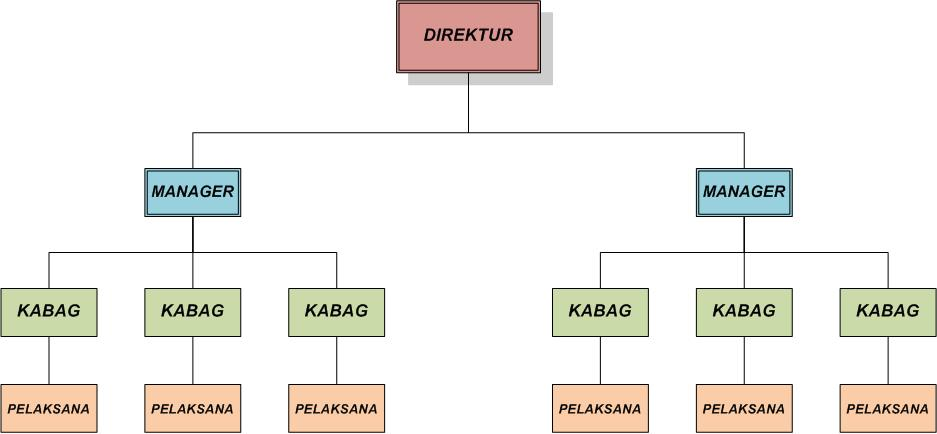
\includegraphics[width=0.90\textwidth]{assets/pics/fig_struktur-organisasi.jpg}}
	\caption{Struktur organisasi perusahaan PT XYZ judul gambar yang panjang lebih dari satu baris}
	\vspace{-1em}
	{\small Sumber: \cite{Widjaja2002a}}
	\label{fig_struktur_organisasi}
\end{figure}



%-----------------------------------------------------------------------------%
% \listoftables
\chapter{\babTiga}


%-----------------------------------------------------------------------------%
% \lipsum[6-6]

%-----------------------------------------------------------------------------%
\section{Kedudukan dan Koordinasi}
%-----------------------------------------------------------------------------%

Selama pelaksanaan kerja magang di PT Ganda Visi Jayatama, peran yang dijalankan berada dalam tim pengembangan sistem CHRIS (Concise Human Resources Information System) sebagai \textit{Backend Engineer Intern}. Tanggung jawab utamanya mencakup pengembangan dan pengujian \textit{Application Programming Interface} (API) yang digunakan oleh sistem, serta kolaborasi dengan anggota tim lainnya dalam penyusunan dan penyempurnaan fitur-fitur sistem kepegawaian berbasis \textit{web}.

\begin{figure}[H]
    \centering
    \fbox{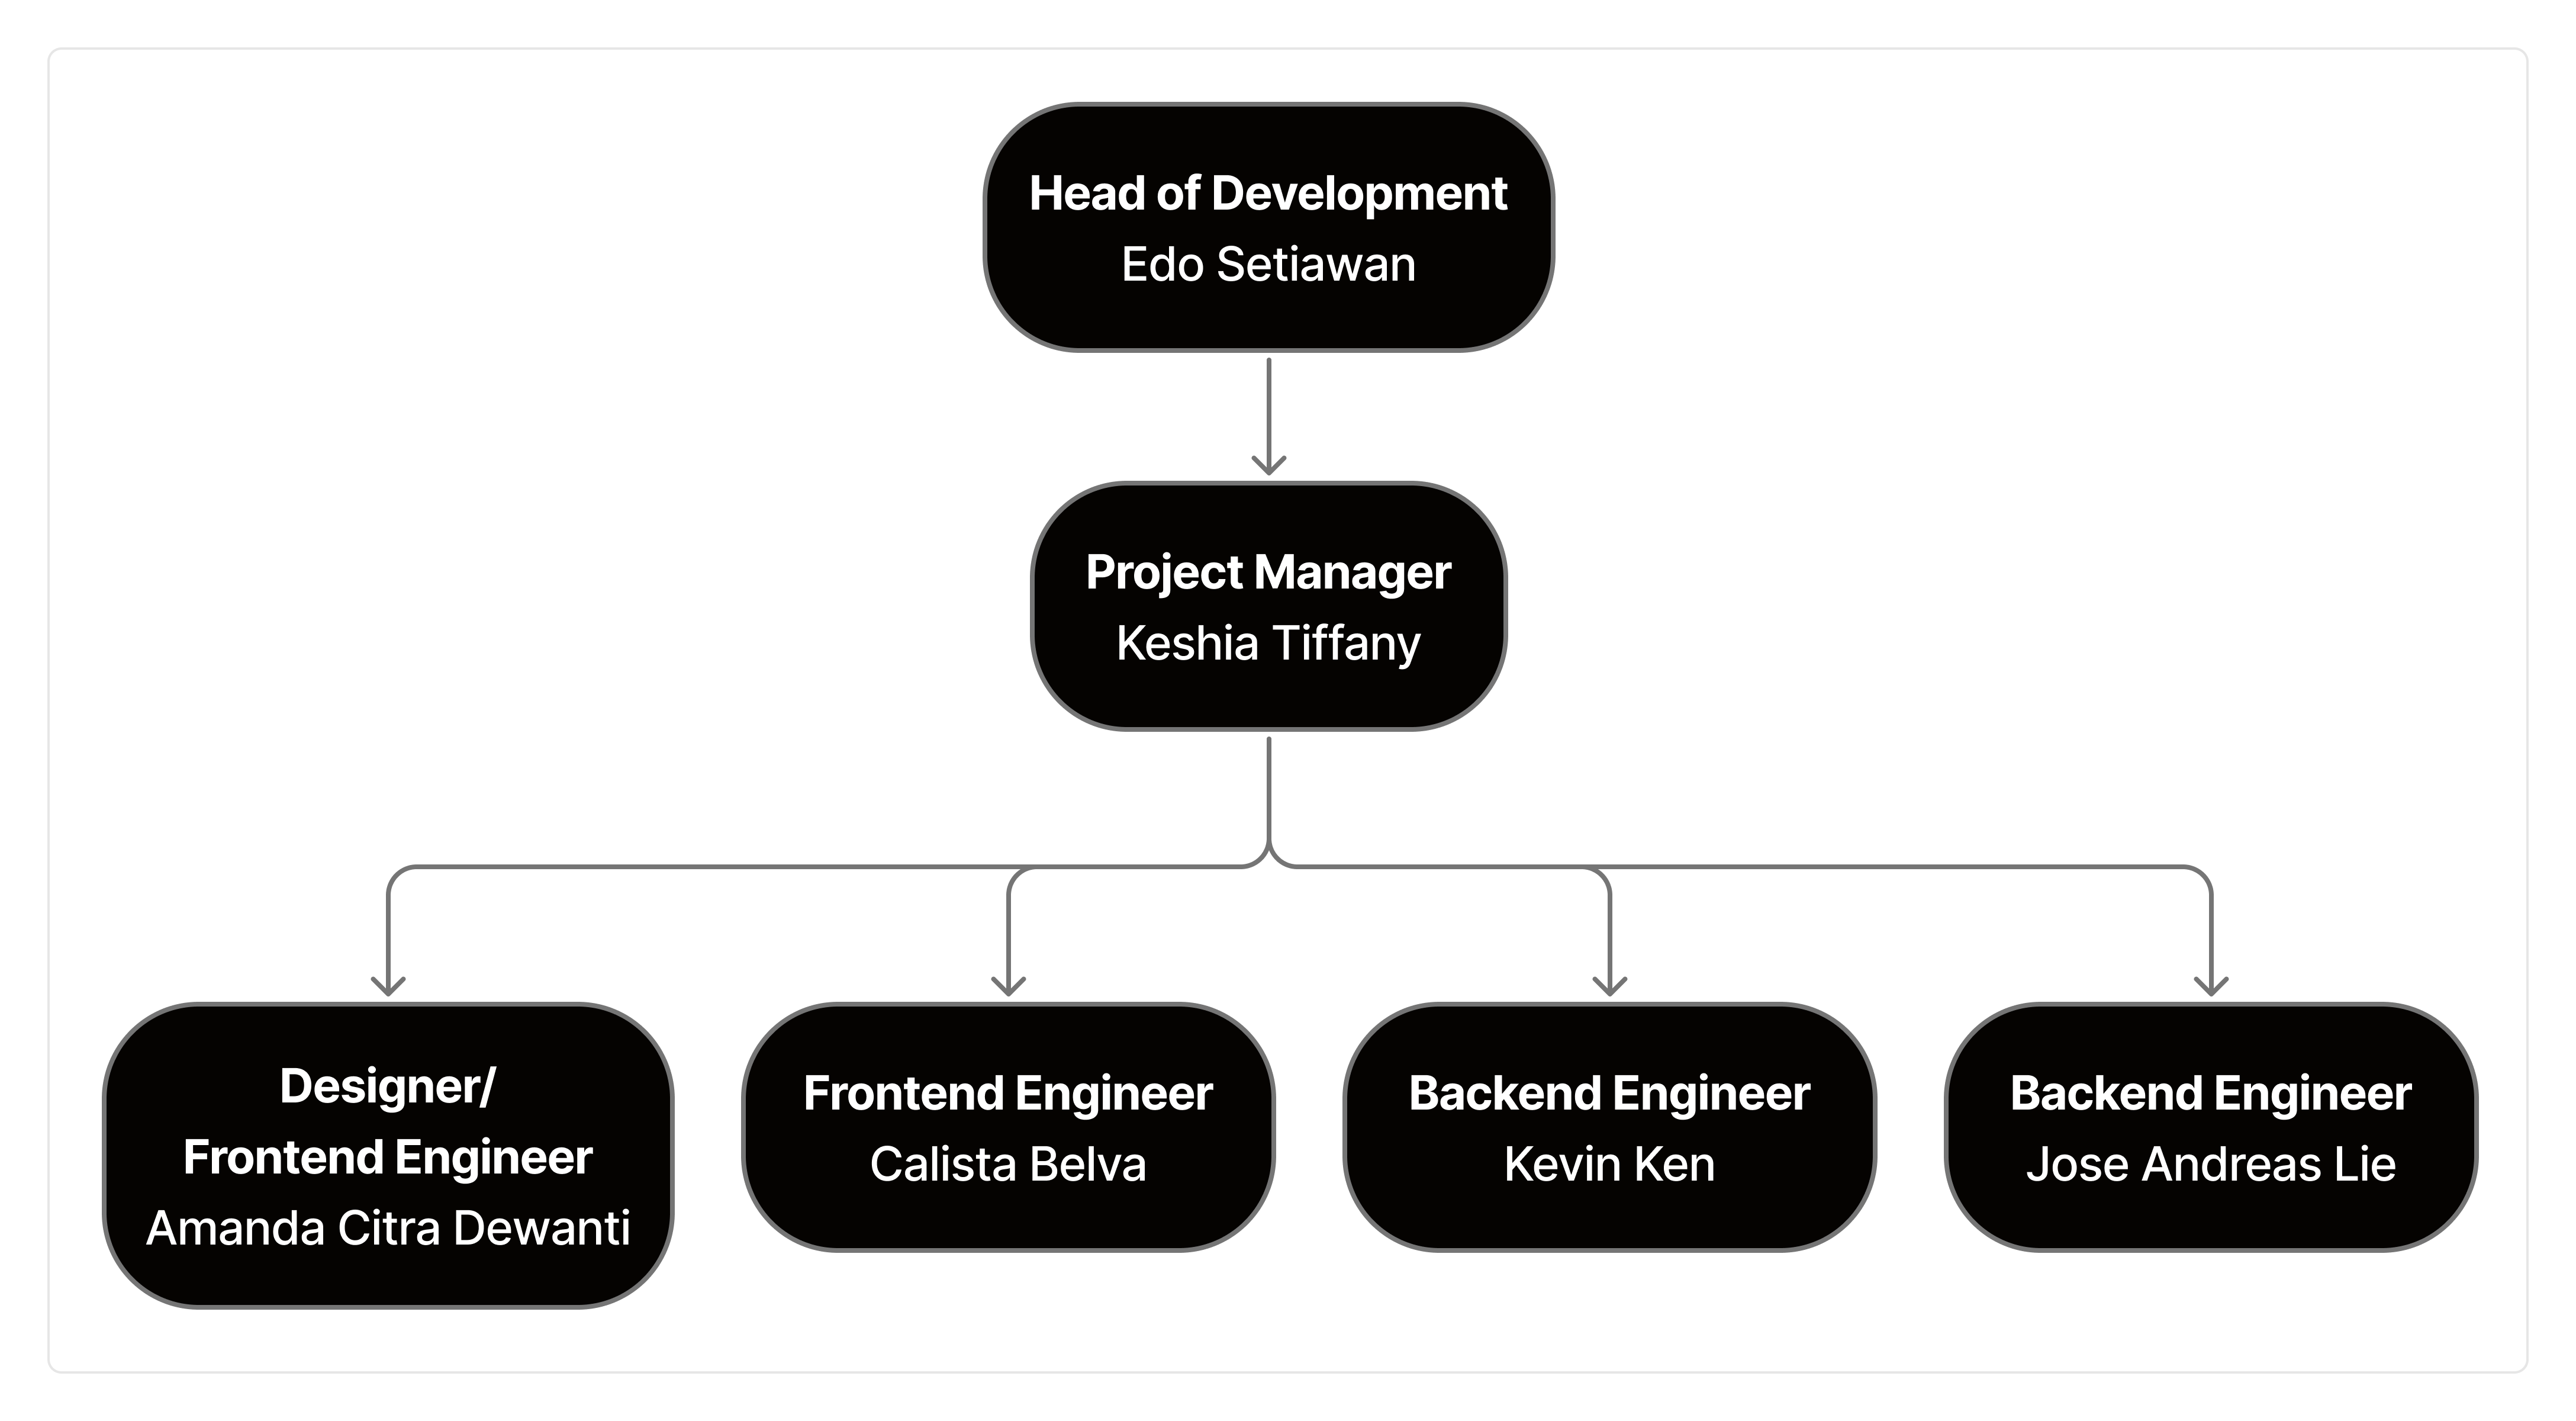
\includegraphics[width=0.8\textwidth]{assets/pics/fig_struktur_tim_chris.png}}
    \caption{Struktur Tim CHRIS}
    \label{fig:struktur_tim_CHRIS}
\end{figure}

Gambar \ref{fig:struktur_tim_CHRIS} merupakan struktur dari tim CHRIS yang terdiri dari sejumlah anggota dengan peran yang saling terintegrasi. Bimbingan diberikan oleh Bapak Edo Setiawan selaku \textit{Supervisor} sekaligus Head of Development, yang secara rutin melaksanakan evaluasi mingguan terhadap progres dan melakukan \textit{code review} atas hasil pengembangan \textit{backend}. Koordinasi teknis lebih lanjut dilaksanakan bersama Bapak Muhammad Alwin Alamsyah Handoko Putra selaku \textit{Backend Lead}, yang memimpin diskusi internal tim \textit{backend} setiap hari Jumat melalui \textit{Backend Internal Meeting}. Perencanaan serta distribusi tugas dikoordinasikan oleh \textit{Project Manager}, Ibu Keshia Tiffany, yang bertanggung jawab dalam pembagian \textit{backlog} kepada anggota tim, serta mengadakan sesi evaluasi pribadi (\textit{one-on-one}) dengan masing-masing anggota tim magang.

Dalam pengembangan tampilan antarmuka sistem, kolaborasi dilakukan bersama \textit{Designer} Amanda Citra Dewanti yang merancang desain akhir dari \textit{web}, serta dua \textit{Frontend Engineer Intern}, Amanda Citra Dewanti dan Calista Belva, yang membangun antarmuka \textit{web} menggunakan React. Sementara itu, pengembangan API menggunakan Express.js dan Node.js, serta pengelolaan basis data dengan PostgreSQL, dijalankan oleh dua Backend Engineer, yaitu Kevin Ken dan satu rekan lainnya dalam tim.

Seluruh kegiatan kerja magang dilakukan secara langsung di kantor (\textit{Work From Office}). Koordinasi dilakukan melalui \textit{daily standup} setiap pagi untuk melaporkan progres harian, menyampaikan rencana kerja, serta mendiskusikan kendala yang dihadapi. Setiap dua minggu sekali, tim juga melaksanakan \textit{sprint retrospective} untuk mengevaluasi hasil kerja dalam satu \textit{sprint} dan menentukan perbaikan serta target \textit{sprint} berikutnya. Penugasan proyek dikelola menggunakan \textit{platform} Jira (Atlassian) dalam bentuk \textit{backlog sprint} yang dibagikan kepada setiap anggota tim secara terstruktur dan terukur.


% \noindent \begin{align}\label{eq:garis}
% 	\cfrac{y - y_{1}}{y_{2} - y_{1}} = 
% 	\cfrac{x - x_{1}}{x_{2} - x_{1}}
% \end{align}

% \equ~\ref{eq:garis} di atas adalah persamaan garis. 
% \equ~\ref{eq:garis} dan \ref{eq:bola} sama-sama dibuat dengan perintah \bslash
% align. 
% Perintah ini juga dapat digunakan untuk menulis lebih dari satu persamaan. 

% \noindent \begin{align}\label{eq:bola}
% 	\underbrace{|\overline{ab}|}_{\text{pada bola $|\overline{ab}| = r$}} 
% 		= \sqrt[2]{(x_{b} - x_{a})^{2} + (y_{b} - y_{a})^{2} + 
% 				\vert\vert(z_{b} - z_{a})^{2}}
% \end{align}

%-----------------------------------------------------------------------------%
\section{Tugas yang Dilakukan}
% \label{sec:multiEqu}
%-----------------------------------------------------------------------------%

Selama pelaksanaan kerja magang di PT Ganda Visi Jayatama, terdapat tanggung jawab utama dalam satu proyek utama, yaitu pengembangan aplikasi \textit{Internal System}. Tugas-tugas yang dijalankan selama magang terbagi ke dalam beberapa aktivitas utama sebagai berikut:

\begin{enumerate}
    \item Mengembangkan API untuk kebutuhan aplikasi \textit{Internal System}, yang mencakup pembuatan fitur-fitur backend sesuai dengan spesifikasi fungsional.
    \item Melakukan dokumentasi terhadap API yang telah dikembangkan menggunakan \textit{platform} dokumentasi API, Apidog.
    \item Melakukan pengujian secara mandiri terhadap API yang dibuat untuk memastikan bahwa seluruh \textit{endpoint} berjalan sesuai dengan fungsinya, serta menangani \textit{error handling} dan validasi data.
\end{enumerate}


% %-----------------------------------------------------------------------------%
\section{Uraian Pelaksanaan Magang}
% -----------------------------------------------------------------------------%
Pelaksanaan kerja magang diuraikan seperti pada Tabel~\ref{tab:tbl_uraian}.

\begin{center}
\begin{longtable}{|c|p{0.75\textwidth}|}
\caption{Pekerjaan yang dilakukan tiap minggu selama pelaksanaan kerja magang}
\label{tab:tbl_uraian} \\
\hline
\textbf{Minggu Ke -} & \textbf{Pekerjaan yang dilakukan} \\
\hline
\endfirsthead

\multicolumn{2}{c}%
{{\parbox{\textwidth}{\centering \tablename\ \thetable{} -- Pekerjaan yang dilakukan tiap minggu selama pelaksanaan kerja magang (lanjutan)}}} \\
\hline
\textbf{Minggu Ke -} & \textbf{Pekerjaan yang dilakukan} \\
\hline
\endhead

\hline \multicolumn{2}{|r|}{{Lanjut pada halaman berikutnya}} \\
\hline
\endfoot

\hline \hline
\endlastfoot

1 & Mempelajari boilerplate backend dan mulai mengembangkan API untuk Employee Status pada sistem CHRIS. \\
\hline
2 & Melanjutkan pengembangan dan penyempurnaan API Employee Status serta melakukan validasi ulang pada form Employee di sistem CHRIS. \\
\hline
3 & Melakukan revisi minor pada API employee form, menyelesaikan tabel User dan Employee Status, serta berpartisipasi dalam Sprint Retro. \\
\hline
4 & Mengembangkan fitur pagination untuk berbagai modul (User, Leave, Attendance), membuat API form pengajuan cuti, serta melakukan code review dan diskusi dalam monthly meeting. \\
\hline
5 & Fokus pada revisi dan pengembangan API perizinan cuti, integrasi dengan frontend, serta showcase sistem CHRIS dan implementasi pagination untuk Leave Types. \\
\hline
6 & Melakukan revisi dan filtering pada Leave Permit Dashboard, menambahkan fitur cancel, serta aktif dalam code review dan weekly meeting tim backend. \\
\hline
7 & Melakukan berbagai pengujian dan UAT untuk Leave Management, membangun sistem tree berbasis jabatan untuk izin, serta menangani revisi migrasi dan API CHRISM (CHRIS Mobile). \\
\hline
8 & Mengembangkan sistem hierarki supervisi berbasis tree, menerapkan biometrik pada login API, dan mulai membangun user report summary API serta mempersiapkan People Report. \\
\hline
9 & Fokus pada penyempurnaan fitur User Report, termasuk penambahan filter tanggal dan perbaikan minor, serta melakukan hashing biometrik dan refactor pada dashboard Leave Permit. \\
\hline
10 &  Memulai riset intensif terkait sistem Payroll dan skema tabelnya, membuat dokumentasi di Apidog.\\
\hline
11 &  Melanjutkan pengembangan API Payroll berdasarkan hasil riset skema tabel, memperbarui dokumentasi di Apidog, serta mengikuti kegiatan Backlog Planning dan Sprint Closing.\\
\hline
12 &  Fokus pada pengembangan lanjutan API Payroll termasuk fitur Create, Get, Update, dan Delete, serta mulai menangani logika data untuk User Allowances.\\
\hline
13 &  Melanjutkan secara intensif pengembangan API Payroll khusus untuk pengelolaan dan perhitungan Each User Allowances secara berkelanjutan sepanjang minggu.\\
\hline
14 &  Mulai mengembangkan dan menyempurnakan Salary Slip APIs serta melakukan bugfix dan refactor pada User Allowance dan konfigurasi Payroll untuk integrasi dengan frontend.\\
\hline
15 &  Menambahkan fitur penghapusan User Allowance, memperbaiki konfigurasi endpoint Payroll, dan membuat API gabungan untuk manajemen detail user, payroll, serta tunjangan.\\
\hline
16 &  Melanjutkan integrasi Salary Slip dengan frontend serta melakukan pengujian menyeluruh terhadap modul Payroll, Allowance, dan Salary Slip.\\
\hline
17 &  Melakukan perbaikan pada logika dan pagination Salary Slip serta Payroll Config, merevisi sistem, dan menyiapkan internal report serta showcase Payroll.\\
\hline

\end{longtable}
\end{center}

% \begin{table}
% 	\centering
% 	\caption{ Pekerjaan yang dilakukan tiap minggu selama pelaksanaan kerja magang}
% 	\label{tbl_uraian}
% 	\begin{tabular}{|c | p{0.75\textwidth}| }
% 		\hline
% 		Minggu Ke - & Pekerjaan yang dilakukan \\
% 		\hline
% 		1 & 
% 		Mempelajari boilerplate backend dan mulai mengembangkan API untuk Employee Status pada sistem CHRIS.\\
% 		\hline
%  		2 & 
% 		Melanjutkan pengembangan dan penyempurnaan API Employee Status serta melakukan validasi ulang pada form Employee di sistem CHRIS.\\
% 		\hline
%  		3 & 
% 		Melakukan revisi minor pada API employee form, menyelesaikan tabel User dan Employee Status, serta berpartisipasi dalam Sprint Retro. \\
%  		\hline
%  		4 & 
% 		Mengembangkan fitur pagination untuk berbagai modul (User, Leave, Attendance), membuat API form pengajuan cuti, serta melakukan code review dan diskusi dalam monthly meeting \\
%  		\hline
%  		5 & 
% 		Fokus pada revisi dan pengembangan API perizinan cuti, integrasi dengan frontend, serta showcase sistem CHRIS dan implementasi pagination untuk Leave Types.\\
%  		\hline
%  		6 & 
% 		Melakukan revisi dan filtering pada Leave Permit Dashboard, menambahkan fitur cancel, serta aktif dalam code review dan weekly meeting tim backend.\\
%  		\hline
%  		7 & 
% 		Melakukan berbagai pengujian dan UAT untuk Leave Management, membangun sistem tree berbasis jabatan untuk izin, serta menangani revisi migrasi dan API CHRISM (CHRIS Mobile).\\
%  		\hline
%  		8 & Mengembangkan sistem hierarki supervisi berbasis tree, menerapkan biometrik pada login API, dan mulai membangun user report summary API serta mempersiapkan People Report.\\
%  		\hline
%  		9 & \\
%  		\hline
%  		10 & \\
%  		\hline
% 	\end{tabular}
% \end{table}



%-----------------------------------------------------------------------------%
\section{Pengumpulan dan Analisis Kebutuhan}
%-----------------------------------------------------------------------------%
Kebutuhan sistem dalam proyek ini diperoleh melalui koordinasi langsung dengan \textit{supervisor} dan tim \textit{backend internal}. Sebagian besar \textit{requirement} ditentukan secara iteratif berdasarkan kebutuhan bisnis dan sprint mingguan yang telah direncanakan oleh tim. Proses pengumpulan \textit{requirement} dilakukan melalui diskusi teknis, \textit{retrospective meeting}, dan \textit{task assignment} harian.

Berikut ini adalah uraian \textit{requirement} utama yang berhasil diidentifikasi dan diimplementasikan dalam proyek selama masa kerja praktik.
%-----------------------------------------------------------------------------%
\subsubsection{Refaktor User Management dan Validasi Data}

Pengembangan dimulai dengan perbaikan sistem \textbf{User Management}, termasuk validasi \textit{form input} dan \textit{refactor} struktur tabel seperti \textit{user} dan \textit{employment status}. Hal ini bertujuan untuk memastikan integritas data pengguna dan kemudahan pengelolaan melalui \textit{backend} maupun \textit{frontend}.
%-----------------------------------------------------------------------------%
\subsubsection{Optimalisasi Leave Permit}

Modul \textbf{Leave Permit} dikembangkan agar lebih efisien dan intuitif. Perubahan meliputi \textit{refactor} pada proses \textit{form submission}, penambahan tombol pembatalan (\textit{cancel}) pengajuan cuti, serta tampilan daftar cuti untuk atasan. Fitur-fitur ini dirancang agar mencerminkan alur persetujuan yang realistis dan terstruktur.
%-----------------------------------------------------------------------------%
\subsubsection{Implementasi Pagination}

Untuk mendukung jumlah data yang besar, sistem pagination ditambahkan pada beberapa modul utama seperti \textbf{User}, \textbf{Leave}, dan \textbf{Attendance}. Hal ini dilakukan guna menjaga performa dan kenyamanan pengguna.
%-----------------------------------------------------------------------------%
\subsubsection{Penambahan Fitur Biometrik untuk CHRIS Mobile}

Fitur biometrik ditambahkan untuk mendukung proses autentikasi pada sistem CHRIS Mobile (CHRISM). Pengguna dapat melakukan login menggunakan data biometrik seperti sidik jari yang telah di-hash dan disimpan dalam kolom khusus pada tabel \textit{users}. Fitur ini ditujukan untuk meningkatkan keamanan serta kenyamanan akses pengguna terhadap sistem.

%-----------------------------------------------------------------------------%
\subsubsection{Pengembangan Sistem Hierarki}

Dibuat fungsi \textit{tree hierarchy} berdasarkan struktur jabatan untuk mendukung fitur-fitur seperti izin cuti (\textit{accept}/\textit{reject}) dan tampilan dashboard atasan. Fungsi ini menjadi dasar logika akses dan pengelolaan hubungan antar pegawai.
%-----------------------------------------------------------------------------%
\subsubsection{Modul Payroll}

Modul \textbf{Payroll} dikembangkan untuk menghasilkan slip gaji setiap bulannya yang dihitung berdasarkan tunjangan. Termasuk di dalamnya pengembangan API untuk CRUD \textit{data payroll}, penyusunan \textit{salary slip}, dan integrasi dengan \textit{frontend}.
%-----------------------------------------------------------------------------%



% ---------------------------------------------------------------------------------%
\section{Perancangan dan Pengembangan Sistem}
% ---------------------------------------------------------------------------------%
Bagian ini menjelaskan perancangan dan pengembangan sistem yang mencakup struktur basis data dan alur sistem untuk fitur-fitur yang dikembangkan selama masa kerja praktik.

% ---------------------------------- %
\subsection{\textit{User Management} dan Validasi Data}
% ---------------------------------- %
Sistem CHRIS\@ telah dilengkapi dengan modul \textit{User Management} yang berfungsi untuk mengelola data pegawai secara efisien. Modul ini mencakup fitur untuk menambahkan, memperbarui, dan menghapus data pegawai, serta melakukan validasi terhadap input yang dimasukkan melalui formulir. Validasi ini bertujuan untuk memastikan bahwa data yang diterima sesuai dengan format dan ketentuan yang berlaku. Meskipun demikian, sejumlah aspek dari modul ini memerlukan penyempurnaan guna meningkatkan integritas data dan mempermudah pengelolaan sistem.

Adapun perbaikan dan pengembangan yang telah dilakukan antara lain:
\begin{itemize}
    \item \textbf{\textit{Refactor User Management}}: Alur pengelolaan data pegawai diperbarui agar setiap entri memiliki status kepegawaian yang terdefinisi dengan baik, sehingga struktur data menjadi lebih sistematis dan mudah diakses.
    \item \textbf{Validasi Form Input}: Validasi terhadap form input ditingkatkan, mencakup pengecekan format email, nomor telepon, serta memastikan bidang yang wajib diisi tidak terlewat, guna mencegah terjadinya inkonsistensi data.
    \item \textbf{Penyempurnaan Struktur Tabel}: Struktur tabel \textit{users} diperbarui dengan menambahkan beberapa referensi eksternal untuk meningkatkan normalisasi data, antara lain:
    \begin{itemize}
        \item Penambahan \textit{employment\_status\_id} yang mereferensikan tabel \textit{employment\_statuses}, menggantikan pendekatan enumerasi yang sebelumnya digunakan secara \textit{hardcoded}.
        \item Penambahan \textit{bank\_id} yang mereferensikan tabel \textit{banks}, menggantikan kolom nama bank dalam bentuk \textit{string} pada tabel \textit{users} untuk menjamin konsistensi data dan memudahkan pengelompokan informasi perbankan.
    \end{itemize}
\end{itemize}

Perubahan ini dilakukan sebagai bagian dari penerapan praktik terbaik dalam pengembangan sistem backend berbasis relasional. Selain itu, modifikasi ini juga memberikan fleksibilitas lebih tinggi dalam pengelolaan data serta meningkatkan skalabilitas modul User Management dalam jangka panjang.

\subsubsection{Diagram ERD User Management}
\begin{figure}[H]
    \centering
    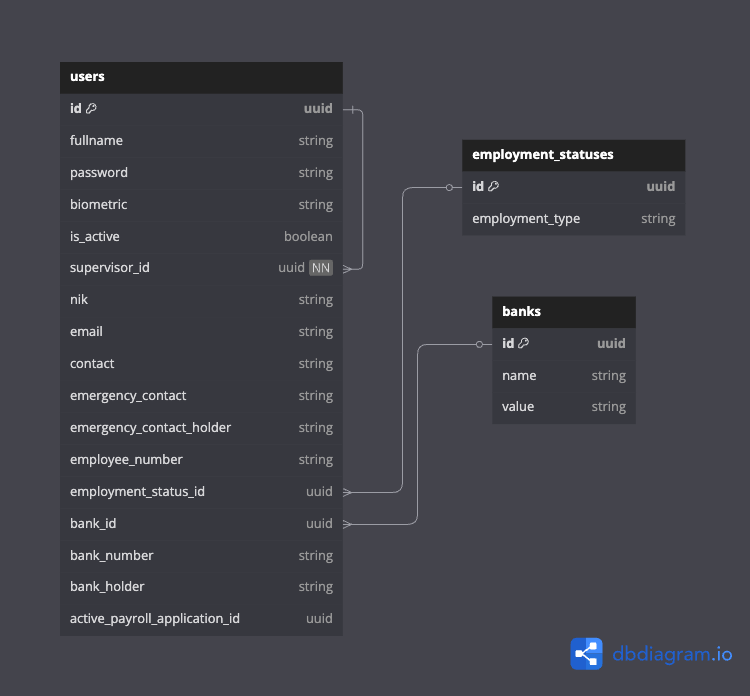
\includegraphics[width=0.8\textwidth]{assets/pics/fig_erd_user_management.png}
    \caption{Diagram ERD untuk modul User Management}
    \label{fig:erd_user_management}
\end{figure}

Gambar \ref{fig:erd_user_management} menunjukkan struktur basis data untuk modul User Management yang telah dimodifikasi. Terdapat beberapa tabel utama yang saling berhubungan, yaitu:
\begin{itemize}
    \item \textbf{Users}: Tabel ini menyimpan data pegawai, termasuk informasi pribadi, status kepegawaian, dan referensi bank.
    \item \textbf{Employment Statuses}: Tabel ini menyimpan berbagai status kepegawaian yang dapat dimiliki oleh pegawai, seperti aktif, cuti, atau tidak aktif.
    \item \textbf{Banks}: Tabel ini menyimpan informasi mengenai bank yang digunakan oleh pegawai untuk penggajian.
\end{itemize}

Sebelumnya modul User Management menggunakan pendekatan \textit{hardcoded} untuk status kepegawaian dan bank, namun kini telah diubah menjadi referensi tabel yang lebih fleksibel. Hal ini memungkinkan penambahan atau perubahan status kepegawaian dan bank tanpa perlu mengubah kode sumber, sehingga meningkatkan efisiensi pengelolaan data.

\subsubsection{Validasi Data pada Formulir User Management}
Validasi data pada formulir \textit{User Management} dilakukan untuk menjamin integritas, konsistensi, dan keamanan data yang masuk ke dalam sistem. Validasi dilakukan baik di sisi \textit{frontend} maupun di sisi \textit{backend}, dengan ketentuan sebagai berikut:

\begin{itemize}
    \item \textbf{\textit{Fullname}}: Nama lengkap pegawai harus diisi dengan format yang benar, yaitu merupakan huruf \textit{alphanumeric}. Validasi ini bertujuan untuk memastikan bahwa nama pegawai dapat dikenali dan diidentifikasi dengan jelas dalam sistem.
    \item \textbf{\textit{Email}}: Hanya alamat email dengan domain \textit{@concise.co.id} yang diperbolehkan. Validasi ini diterapkan untuk memastikan bahwa hanya pegawai internal yang terdaftar di sistem. Format email juga diverifikasi menggunakan ekspresi reguler untuk menghindari entri tidak valid.
    \item \textbf{NIK}: Nomor Induk Kependudukan (NIK) harus diisi dengan format yang benar, yaitu terdiri dari 16 digit angka. Validasi ini penting untuk memastikan bahwa NIK yang dimasukkan sesuai dengan standar yang berlaku di Indonesia.
    \item \textbf{\textit{Contact}}: Hanya nomor telepon yang dimulai dengan \textit{prefix} \textit{+62} atau \textit{0} yang diterima. Validasi ini bertujuan untuk memastikan bahwa nomor telepon yang dimasukkan sesuai dengan format nomor telepon pada umumnya.
    \item \textbf{\textit{Emergency Contact}}: Sama seperti nomor telepon, hanya nomor yang dimulai dengan \textit{prefix} \textit{+62} atau \textit{0} yang diterima. Hal ini untuk memastikan bahwa kontak darurat yang dimasukkan dapat dihubungi dengan mudah.
    \item \textbf{\textit{Bank Holder}}: Nama pemegang rekening bank harus diisi dengan format yang benar, yaitu merupakan huruf \textit{alphanumeric}. Validasi ini bertujuan untuk memastikan bahwa nama pemegang rekening sesuai dengan nama pegawai yang terdaftar dalam sistem.
    \item \textbf{\textit{Bank Account Number}}: Validasi dilakukan untuk memastikan bahwa nomor rekening bank yang dimasukkan hanya terdiri dari angka. Hal ini penting untuk menghindari kesalahan dalam proses penggajian.
\end{itemize}

Validasi ini tidak hanya berfungsi untuk memperbaiki pengalaman pengguna, tetapi juga mencegah terjadinya kesalahan logika dan duplikasi data di tingkat basis data. Seluruh ketentuan ini dirancang berdasarkan standar praktik terbaik dalam pengelolaan data karyawan di lingkungan perusahaan.

% ---------------------------------- %
\subsection{Leave Permit}
% ---------------------------------- %
Modul \textit{Leave Permit} merupakan fitur yang memungkinkan pegawai mengajukan permohonan cuti, serta memberikan wewenang kepada atasan untuk menyetujui atau menolak permohonan tersebut. Setiap jenis cuti memiliki jatah tersendiri, dan modul ini juga berfungsi untuk menghitung secara otomatis sisa cuti yang dimiliki oleh masing-masing pegawai. Sistem ini dirancang untuk mencerminkan alur persetujuan yang terstruktur dan realistis, dengan memperhatikan hierarki jabatan di dalam perusahaan.

Sistem ini sudah pernah digunakan sebelumnya, namun mengalami beberapa kendala yang perlu diperbaiki. Beberapa perbaikan yang dilakukan antara lain adalah:
\begin{itemize}
    \item \textbf{Refactor Form Submission}: Proses pengajuan cuti ditambahkan \textit{officer in charge} (\textit{oic}) dengan tujuan sebagai pengganti pegawai saat ia cuti.
    \item \textbf{Cancel Button}: Ditambahkan fitur pembatalan (\textit{cancel}) pengajuan cuti, sehingga pegawai dapat membatalkan permohonan yang belum disetujui.
    \item \textbf{Leave Permit Dashboard}: Tampilan daftar cuti ditampilkan di \textit{home page} supaya semua pegawai dapat melihat siapa saja yang mengajukan cuti di minggu itu.
\end{itemize}


\subsubsection{Diagram ERD Leave Permit}
\begin{figure}[H]
    \centering
    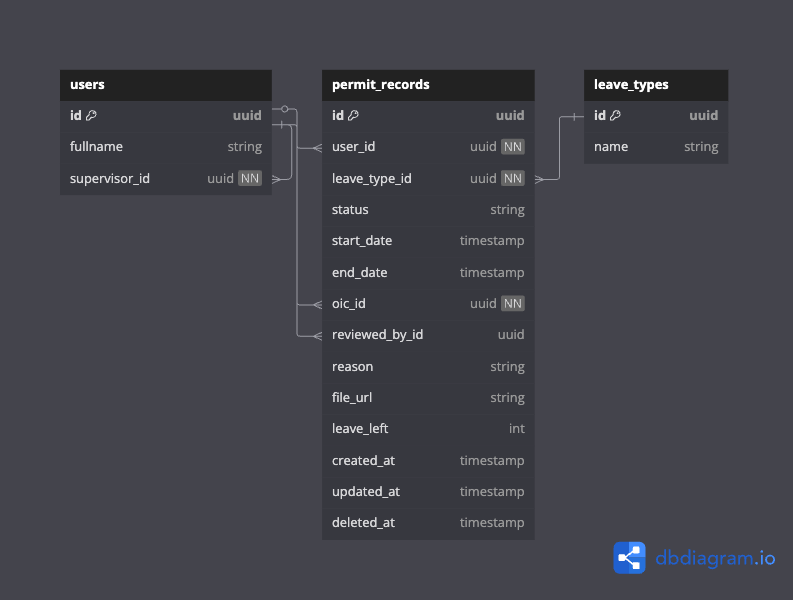
\includegraphics[width=0.8\textwidth]{assets/pics/fig_erd_leave_permit.png}
    \caption{Diagram ERD untuk modul Leave Permit}
    \label{fig:erd_leave_permit}
\end{figure}

Gambar \ref{fig:erd_leave_permit} menunjukkan struktur basis data untuk modul Leave Permit yang dimodifikasi. Terdapat beberapa tabel utama yang saling berhubungan, yaitu:
\begin{itemize}
    \item \textbf{User}: Tabel ini menyimpan data pegawai yang mengajukan cuti, termasuk informasi pribadi dan status kepegawaian.
    \item \textbf{Leave Types}: Tabel ini menyimpan jenis-jenis cuti yang tersedia, termasuk nama, deskripsi, dan jatah cuti yang diberikan kepada pegawai.
    \item \textbf{Permit Records}: Tabel ini menyimpan data permohonan cuti yang diajukan oleh pegawai, termasuk tanggal pengajuan, tanggal mulai dan selesai cuti, status persetujuan, dan pegawai lain yang menggantikan dia sebagai \textit{office in charge}.
\end{itemize}


\subsubsection{Alur Sistem Leave Permit}

\begin{figure}[H]
    \centering
    \fbox{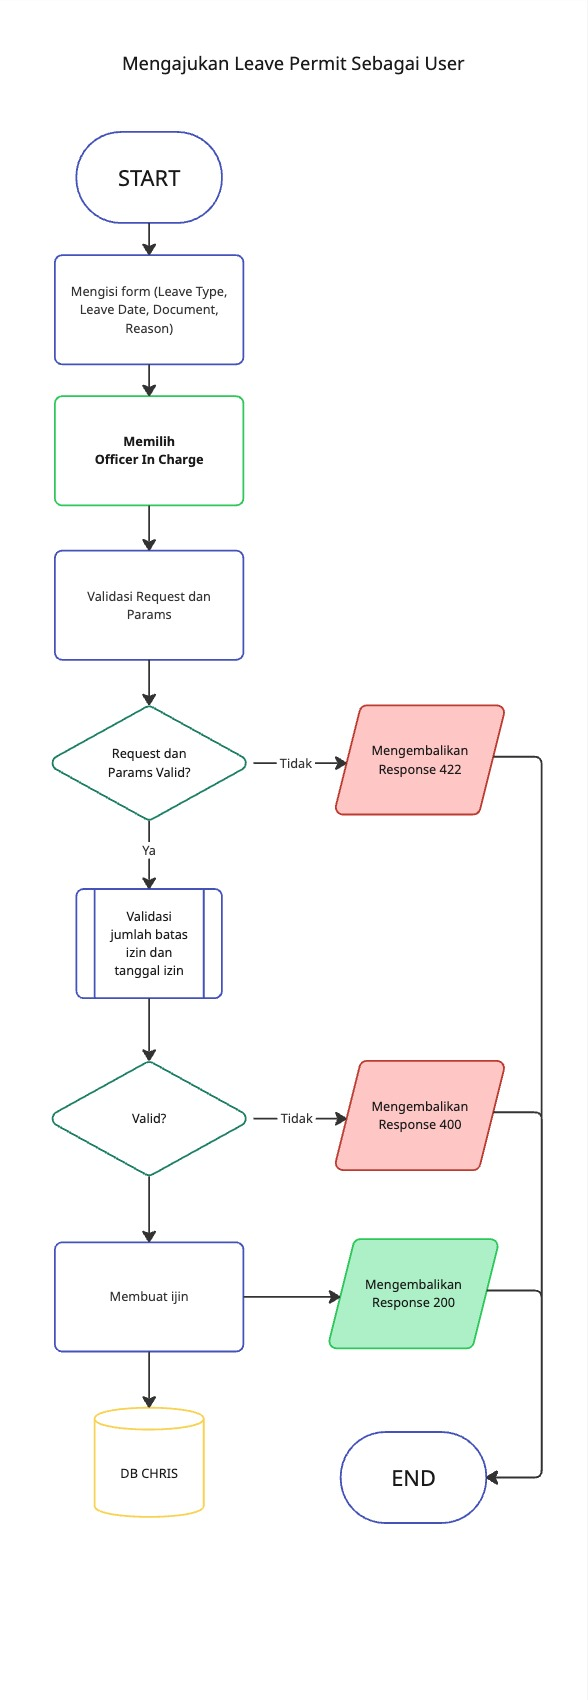
\includegraphics[height=0.8\textheight]{assets/pics/fig_mengajukan_leave_permit_sebagai_user.jpg}}
    \caption{\textit{Flowchart} alur sistem Leave Permit}
    \label{fig:flowchart_leave_permit}
\end{figure}

Gambar \ref{fig:flowchart_leave_permit} menunjukkan alur sistem \textit{Leave Permit} yang diawali oleh pegawai yang mengajukan cuti melalui formulir yang tersedia. Informasi yang diisi mencakup jenis cuti, rentang tanggal, alasan pengajuan, serta penunjukan \textit{officer in charge} sebagai pengganti selama periode cuti. Setelah permohonan dikirimkan, sistem akan menyimpan data ke dalam tabel \textit{Permit Records}, dan atasan dapat memberikan persetujuan atau penolakan. Selama permohonan belum diproses, pegawai memiliki opsi untuk membatalkannya. Jika disetujui, sistem secara otomatis akan memperbarui sisa jatah cuti sesuai jenis cuti yang diajukan. Status pengajuan dapat dipantau melalui dashboard yang menampilkan daftar cuti yang aktif dalam minggu berjalan.

Sebagai bagian dari pengembangan lanjutan modul ini, dilakukan penyesuaian struktur data dengan menambahkan kolom \textit{oic\_id} pada tabel \textit{Permit Records}. Penambahan ini ditujukan untuk memenuhi kebutuhan bisnis dalam menjamin kesinambungan operasional saat pegawai cuti, dengan menunjuk rekan kerja yang bertanggung jawab selama periode tersebut. Perubahan ini turut memperkuat logika bisnis sistem dan memastikan distribusi tugas tetap berjalan secara efisien.


\subsubsection{Alur Sistem Cancel Leave Permit}
\begin{figure}[H]
    \centering
    \fbox{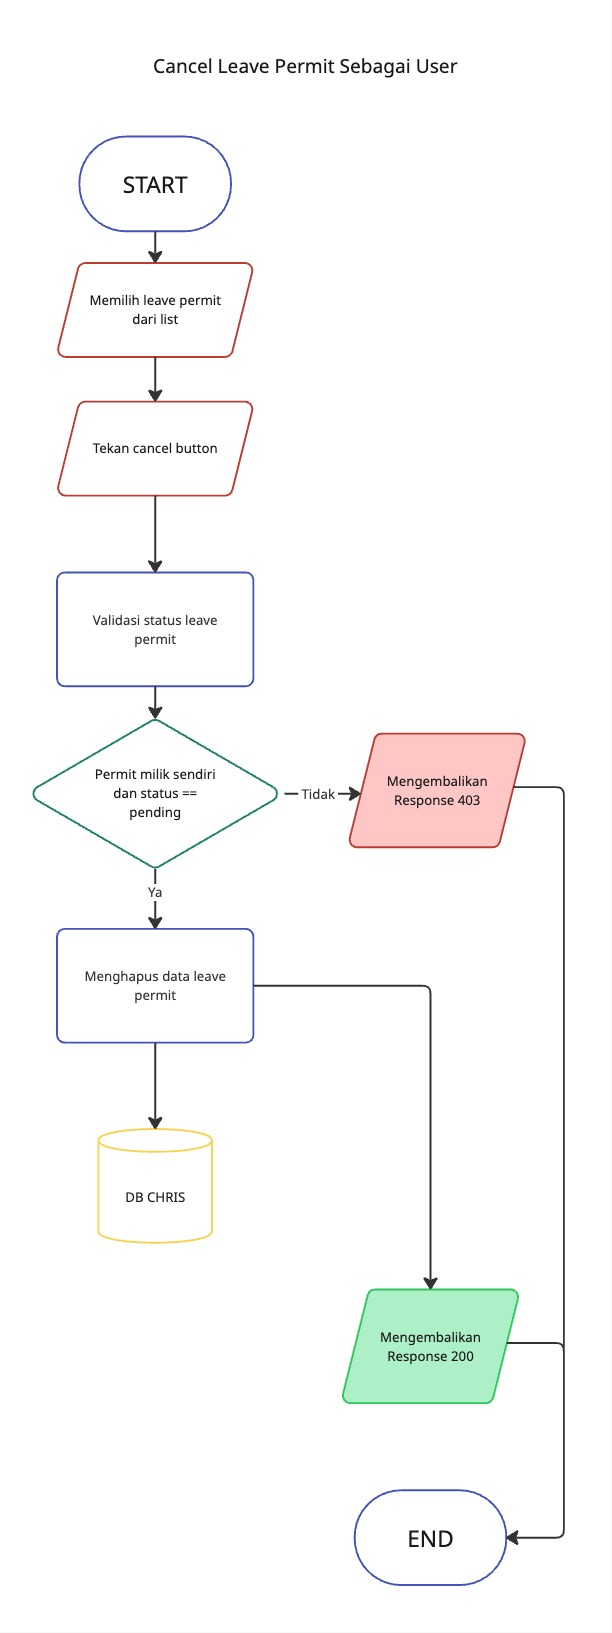
\includegraphics[height=0.8\textheight]{assets/pics/fig_cancel_leave_permit_sebagai_user.jpg}}
    \caption{\textit{Flowchart} alur sistem Cancel Leave Permit}
    \label{fig:flowchart_cancel_leave_permit}
\end{figure}

Gambar \ref{fig:flowchart_cancel_leave_permit} menggambarkan alur proses pembatalan permohonan cuti oleh pegawai. Setelah pengajuan dilakukan, pegawai dapat membatalkan permohonan selama statusnya belum disetujui oleh atasan. Permintaan pembatalan dikirim melalui formulir yang tersedia, kemudian sistem akan memverifikasi status permohonan. Jika permohonan belum disetujui, sistem akan melakukan \textit{soft delete} pada data di tabel \textit{Permit Records}. Namun, apabila permohonan telah disetujui, sistem akan menolak proses pembatalan dan menampilkan notifikasi kesalahan bahwa pengajuan tidak dapat dibatalkan.

\subsubsection{Alur Sistem Leave Permit Dashboard}
Alur pengambilan dan penampilan data cuti pada halaman \textit{dashboard} digunakan untuk menampilkan pegawai-pegawai yang sedang cuti di minggu berjalan. Proses dimulai saat pegawai mengakses dashboard dan sistem kemudian melakukan query terhadap data \textit{permit records} yang memiliki rentang tanggal cuti berada dalam minggu berjalan dan status pengajuan sudah aktif. Data yang diambil mencakup nama pegawai, jenis cuti, tanggal mulai dan selesai, serta \textit{officer in charge} yang ditunjuk.

Informasi tersebut disajikan dalam bentuk tabel agar mudah dipahami dan dapat digunakan oleh pegawai untuk mengetahui siapa saja yang sedang atau akan cuti, serta mengetahui siapa rekan pengganti yang dapat dihubungi untuk keperluan operasional. Fitur ini ditujukan untuk meningkatkan transparansi dan mendukung koordinasi lintas tim selama periode cuti berlangsung.


% ---------------------------------- %
\subsection{Fitur Autentikasi Biometrik pada CHRIS Mobile}
% ---------------------------------- %
Sebagai bagian dari pengembangan sistem CHRIS Mobile (CHRISM), ditambahkan fitur autentikasi berbasis biometrik untuk meningkatkan kenyamanan dan keamanan akses pengguna. Implementasi ini dilakukan dengan menambahkan kolom baru biometric pada tabel \textit{users}. Kolom ini menyimpan hasil \textit{hash} sepanjang maksimal 255 karakter dari data biometrik pengguna seperti sidik jari.

Fitur ini memberikan alternatif \textit{login} selain kata sandi serta mendukung praktik keamanan modern, termasuk \textit{multi-factor authentication}. Karena data biometrik telah melalui proses hashing, informasi yang disimpan tetap aman dan tidak dapat digunakan kembali secara langsung. Fitur ini hanya tersedia pada aplikasi CHRIS Mobile dan tidak memengaruhi sistem versi web atau \textit{desktop}.

\subsubsection{Alur Register Biometrik}
\begin{figure}[H]
    \centering
    \fbox{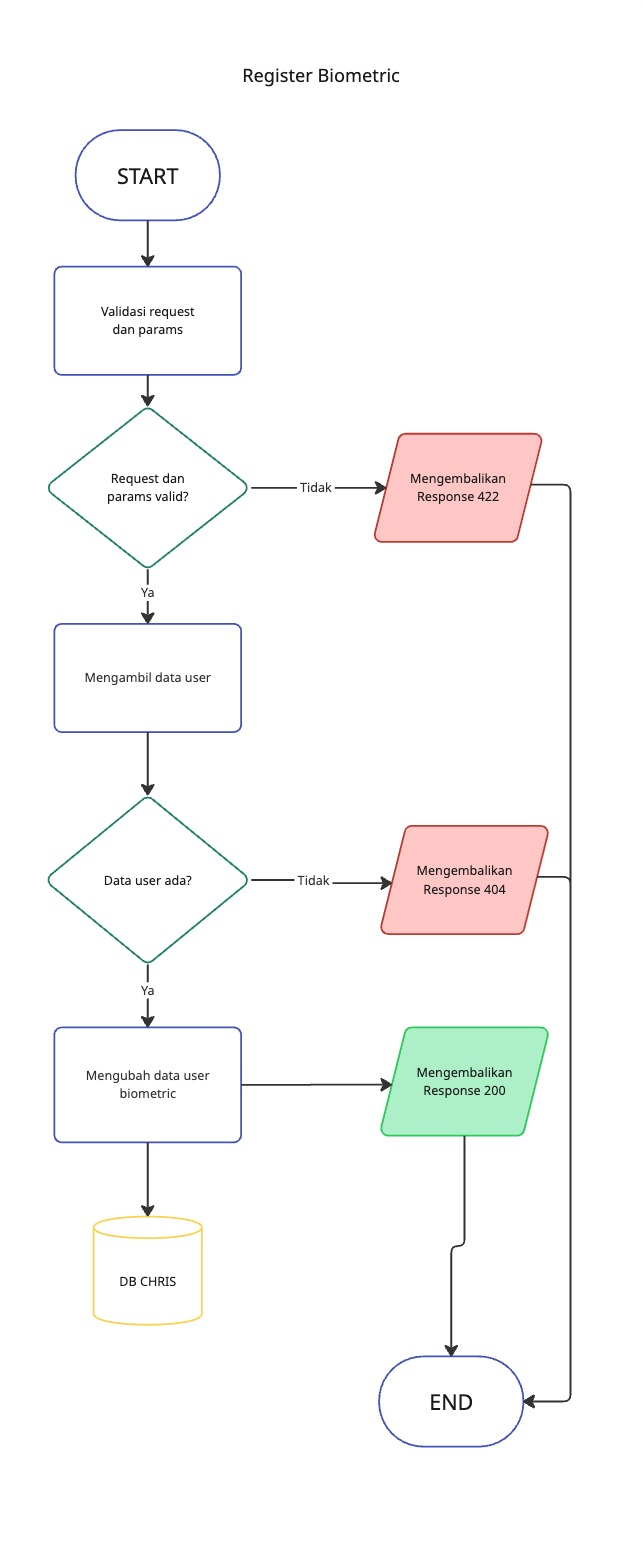
\includegraphics[height=0.8\textheight]{assets/pics/fig_register_biometric.jpg}}
    \caption{\textit{Flowchart} alur sistem registrasi biometrik pada CHRIS Mobile}
    \label{fig:flowchart_register_biometrik_chris_mobile}
\end{figure}
Gambar \ref{fig:flowchart_register_biometrik_chris_mobile} menunjukkan alur sistem registrasi dan autentikasi biometrik pada aplikasi CHRIS Mobile (CHRISM). Proses dimulai ketika pengguna mengakses halaman profil dan memilih opsi “\textit{Activate Biometric}”. Setelah itu, aplikasi akan memicu pemindaian biometrik menggunakan sensor sidik jari pada perangkat. Jika proses pemindaian berhasil, sistem akan secara otomatis menghasilkan \textit{random} string sepanjang 255 karakter yang mewakili identitas biometrik pengguna. Nilai ini kemudian dikirimkan ke \textit{backend} melalui API khusus untuk proses pendaftaran biometrik.

Di sisi \textit{backend}, data tersebut akan di-hash dan disimpan pada kolom \textit{biometric} di tabel \textit{users} untuk keperluan autentikasi selanjutnya.

Dalam implementasi autentikasi, saat aplikasi dibuka, CHRISM\@ akan kembali meminta verifikasi biometrik dari perangkat. Jika sidik jari cocok, sistem akan menembakkan \textit{payload} berupa \textit{random string} 255 karakter yang identik dengan yang telah didaftarkan sebelumnya, lalu mengirimkannya ke \textit{endpoint login biometrik}. \textit{Backend} akan mencocokkan hasil \textit{hash} dari \textit{string} tersebut dengan data yang tersimpan di basis data. Jika sesuai, maka autentikasi dinyatakan berhasil dan pengguna dapat langsung masuk ke sistem tanpa perlu menggunakan kata sandi. Proses ini dirancang untuk meningkatkan keamanan serta memberikan pengalaman masuk aplikasi yang lebih praktis dan efisien bagi pengguna CHRISM\@.

\subsubsection{Alur Autentikasi Login Menggunakan Biometrik}
\begin{figure}[H]
    \centering
    \fbox{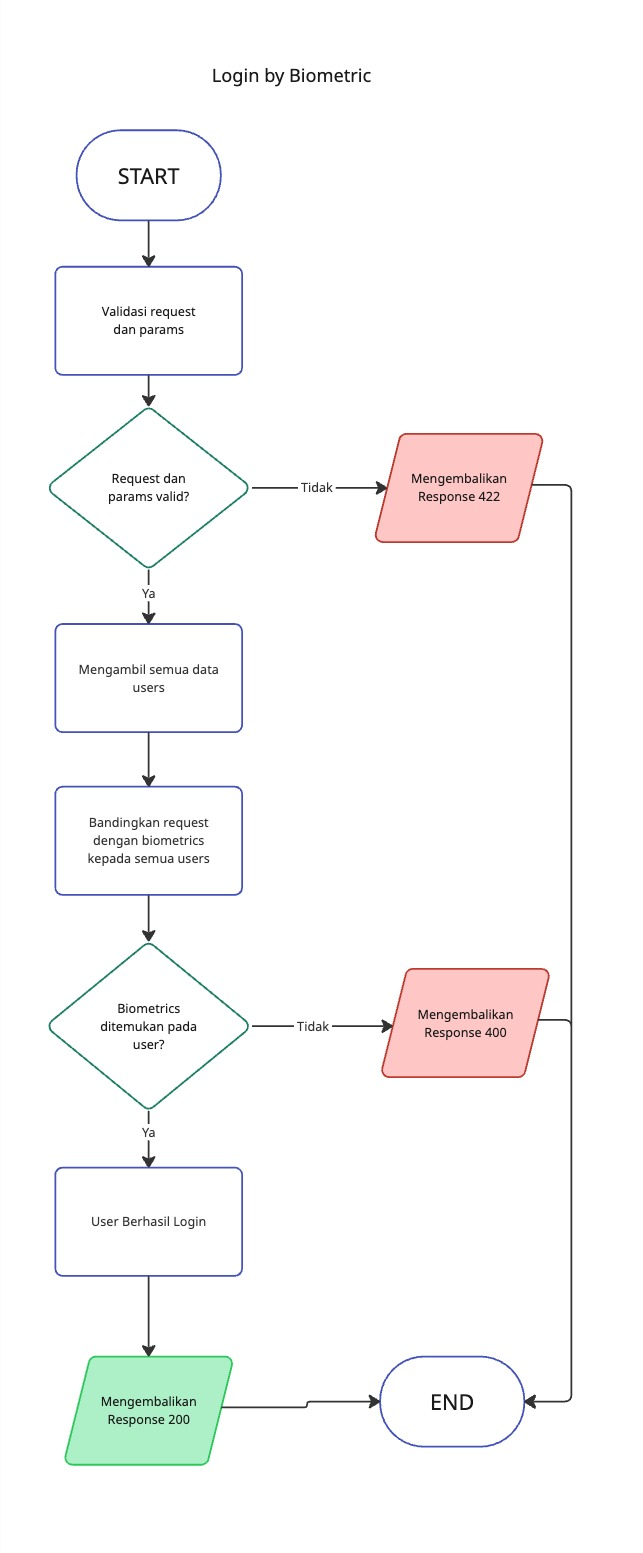
\includegraphics[height=0.8\textheight]{assets/pics/fig_login_by_biometric.jpg}}
    \caption{\textit{Flowchart} alur sistem autentikasi biometrik pada CHRIS Mobile}
    \label{fig:flowchart_autentikasi_biometrik_chris_mobile}
\end{figure}
Gambar \ref{fig:flowchart_autentikasi_biometrik_chris_mobile} menunjukkan alur sistem autentikasi biometrik pada CHRIS Mobile. Proses dimulai ketika pengguna memilih opsi \textit{login} menggunakan biometrik. Sistem kemudian akan meminta data biometrik dari perangkat, yang selanjutnya di-hash dan dibandingkan dengan data yang tersimpan di basis data. Jika cocok, pengguna akan berhasil masuk ke dalam aplikasi. Jika tidak, sistem akan menampilkan pesan kesalahan dan meminta pengguna untuk mencoba kembali. Fitur ini dirancang untuk memberikan pengalaman pengguna yang lebih cepat dan aman, serta mengurangi ketergantungan pada kata sandi yang dapat dilupakan atau dicuri.



% ---------------------------------- %
\subsection{Sistem Hierarki Supervisi}
% ---------------------------------- %
Sistem CHRIS\@ menerapkan struktur hierarki berbasis pohon (\textit{tree hierarchy}) untuk mengelola hubungan antara pegawai dan atasan. Modul-modul dalam sistem ini, seperti pengajuan cuti, bergantung pada struktur tersebut, di mana permohonan cuti hanya dapat disetujui oleh atasan langsung dari pegawai yang bersangkutan.

Diagram pada Gambar \ref{fig:logika_fungsi_hierarki_mencari_semua_bawahan} menggambarkan alur logika sistem dalam mencari seluruh bawahan dari seorang pegawai. Fungsi ini dimulai dengan mengambil seluruh data pengguna dari basis data, kemudian melakukan pencarian rekursif terhadap pegawai yang memiliki \textit{supervisor\_id} yang sesuai dengan \textit{id} pegawai tersebut. Pencarian dilakukan secara berlapis hingga seluruh struktur bawahan ditemukan.

\begin{figure}
    \centering
    \fbox{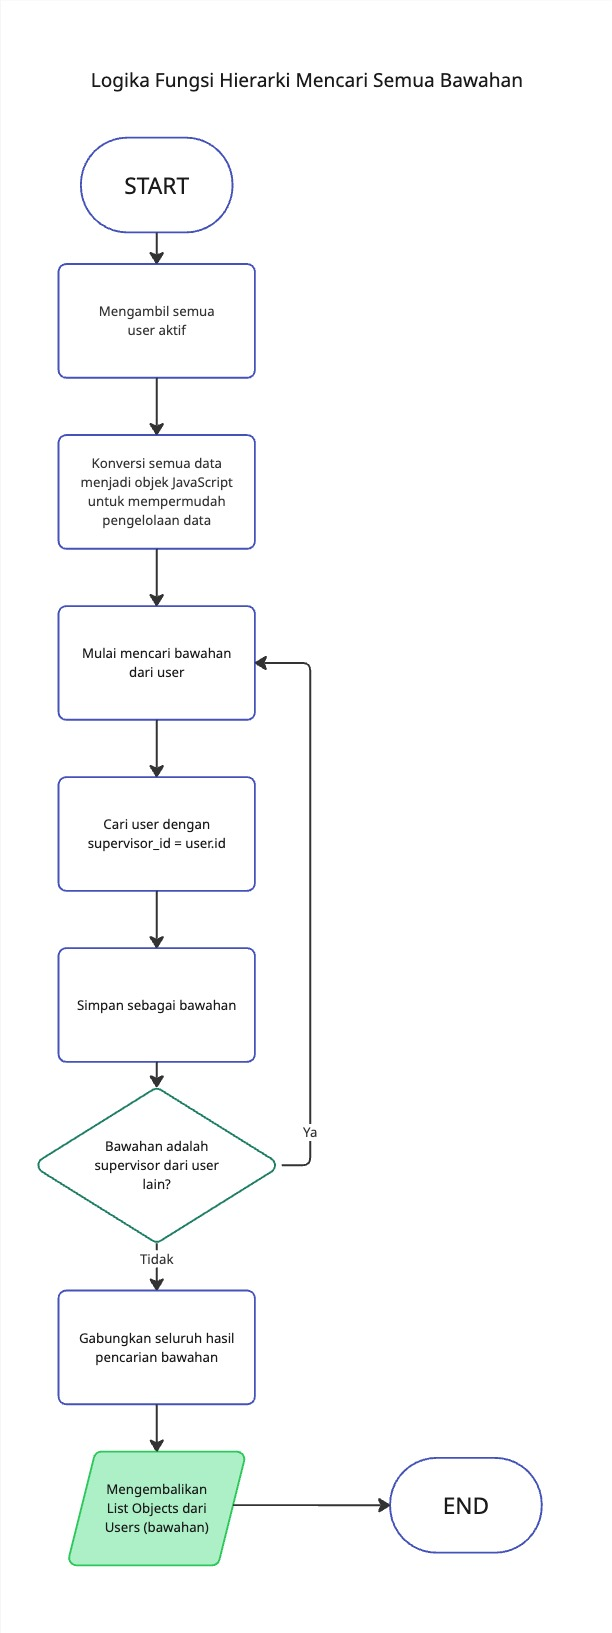
\includegraphics[height=0.8\textheight]{assets/pics/fig_logika_fungsi_hierarki_mencari_semua_bawahan.jpg}}
    \caption{Logika Fungsi Hierarki untuk Mencari Semua Bawahan}
    \label{fig:logika_fungsi_hierarki_mencari_semua_bawahan}
\end{figure}

Dengan pendekatan ini, sistem mampu menentukan siapa saja yang berada dalam rantai struktur supervisi, baik secara langsung maupun tidak langsung. Hal ini memungkinkan sistem untuk secara efisien menetapkan pihak yang berwenang dalam proses seperti persetujuan cuti, pelacakan struktur organisasi, maupun pengelolaan akses modul internal.

Fungsi ini telah digunakan secara langsung dalam modul \textit{Leave Permit} untuk memastikan bahwa pengajuan cuti hanya dapat ditinjau dan disetujui oleh atasan yang sesuai. Selain itu, logika ini juga dapat diterapkan pada modul lain yang membutuhkan pemetaan hubungan antarpegawai secara hierarkis, seperti monitoring kinerja, delegasi tugas, atau manajemen tim lintas divisi.

% {\footnotesize
% \begin{lstlisting}[basicstyle=\linespread{0.8}, caption= Potongan Kode untuk mendapatkan bawahan-bawahan dari \textit{Supervisor}, label= code:hierarchy_functions]

% export async function checkChildren(userId: string): Promise<any[]> {
%     try {
%         // Get all users from the database
%         const allUsers = await models.user.findAll({
%             attributes: ['id', 'fullname', 'supervisor_id'],
%             where: {
%                 is_active: true,
%                 deleted_at: null,
%             },
%         });

%         // Convert to plain objects for easier manipulation
%         const users = allUsers.map((user) => user.get({ plain: true }));

%         // Find direct subordinates (users whose supervisor_id matches the userId)
%         const findSubordinates = (parentId: string): any[] => {
%             // Find direct subordinates
%             const directSubordinates = users.filter((user) => user.supervisor_id === parentId);

%             // For each direct subordinate, find their subordinates recursively
%             let allSubordinates = [...directSubordinates];

%             directSubordinates.forEach((subordinate) => {
%                 const childSubordinates = findSubordinates(subordinate.id);
%                 allSubordinates = [...allSubordinates, ...childSubordinates];
%             });

%             return allSubordinates;
%         };

%         return findSubordinates(userId);
%     } catch (error) {
%         console.log('Error finding subordinates:', error);
%         throw error;
%     }
% }

% // if you only need the ids of the subordinates, use this function!
% export async function checkChildrenIds(userId: string): Promise<string[]> {
%     const subordinates = await checkChildren(userId);
%     return subordinates.map((subordinate) => subordinate.id);
% }

% \end{lstlisting}
% }



% ---------------------------------- %
\subsection{Payroll}
% ---------------------------------- %
Modul \textit{Payroll} merupakan salah satu fitur utama dalam sistem CHRIS\@. Modul ini bertujuan untuk mengelola data penggajian pegawai, termasuk perhitungan gaji berdasarkan tunjangan yang telah ditentukan.

\subsubsection{Diagram ERD Payroll}
\begin{figure}[H]
    \centering
    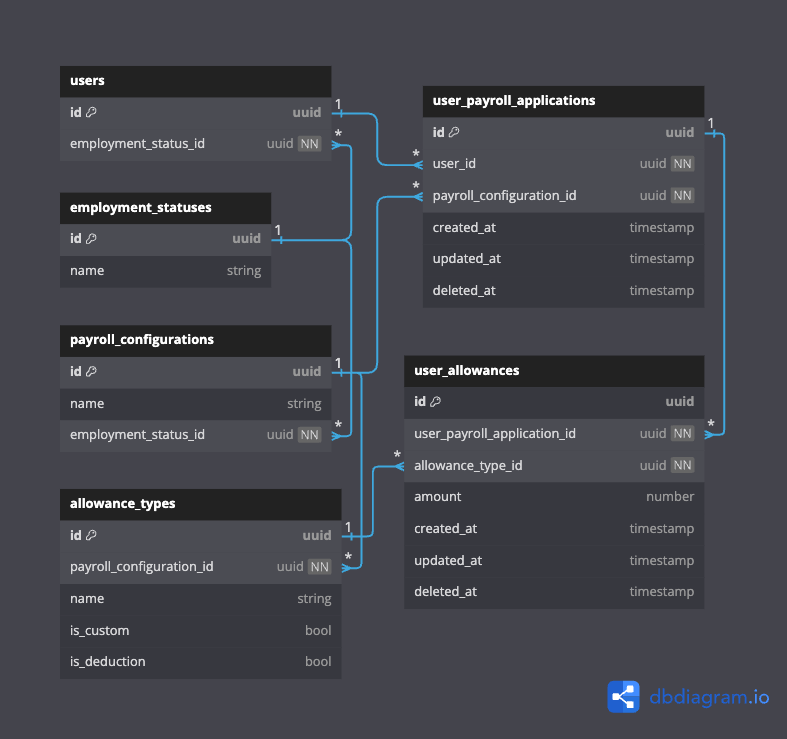
\includegraphics[width=0.8\textwidth]{assets/pics/fig_erd_payroll.png}
    \caption{Diagram ERD untuk modul Payroll}
    \label{fig:erd_payroll}
\end{figure}

Struktur basis data untuk modul Payroll terdiri dari beberapa tabel utama yang saling berhubungan. Berikut adalah penjelasan singkat mengenai tabel-tabel tersebut:
\begin{itemize}
    \item \textbf{User}: Tabel ini menyimpan data pegawai yang mencakup informasi pribadi, status kepegawaian, dan referensi ke konfigurasi penggajian yang digunakan.
    \item \textbf{Employment Status}: Tabel ini menyimpan data status kepegawaian yang digunakan sebagai referensi pada berbagai modul dalam sistem, salah satunya adalah modul \textit{Payroll}.
    \item \textbf{Payroll Configuration}: Tabel ini menyimpan konfigurasi penggajian yang mencakup nama, status kepegawaian, dan tunjangan yang berlaku. Setiap konfigurasi dapat memiliki beberapa tunjangan yang terkait.
    \item \textbf{Allowances Types}: Tabel ini menyimpan jenis-jenis tunjangan yang tersedia pada payroll configuraion yang telah dibuat, dan juga tunjangan tambahan untuk pegawai tertentu. Setiap jenis tunjangan memiliki nama, dan tipe (tunjangan atau potongan).
    \item \textbf{User Payroll Application}: Tabel ini menyimpan data Payroll yang telah diisi oleh \textit{Superadmin} untuk setiap pegawai.
    \item \textbf{User Allowances}: Tabel ini menyimpan data tunjangan spesifik untuk setiap pegawai. Tabel ini berisi informasi mengenai jenis tunjangan, jumlah, dan referensi ke pegawai yang bersangkutan.
\end{itemize}

\subsubsection{Alur Sistem Payroll}
Alur sistem \textit{Payroll} diawali dengan pembuatan data \textit{Payroll Configuration}, yang mencakup nama konfigurasi, status kepegawaian (\textit{Employment Status}), serta daftar tunjangan (\textit{Allowances}) yang berlaku. Setelah konfigurasi dibuat, \textit{Superadmin} melanjutkan ke modul \textit{User Management} untuk mengatur data gaji setiap pegawai secara individual.

Dalam modul \textit{User Management}, \textit{Superadmin} memilih \textit{Payroll Configuration} berdasarkan status kepegawaian pengguna, mengisi besaran gaji pokok, serta melengkapi jumlah masing-masing tunjangan yang ditetapkan. Selain itu, \textit{Superadmin} juga dapat menambahkan tunjangan (\textit{allowance}) atau potongan (\textit{deduction}) khusus yang hanya berlaku bagi pengguna tersebut, guna menyesuaikan skema gaji secara fleksibel.

Setelah data selesai disimpan, \textit{Superadmin} dapat mengakses modul \textit{Salary Slip} untuk melakukan finalisasi gaji. Finalisasi ini memungkinkan pengecekan akhir terhadap rincian gaji sebelum tanggal gajian. Di PT Ganda Visi Jayatama, proses penggajian dilakukan setiap tanggal 25, sehingga proses finalisasi disarankan dilakukan pada tanggal 24 setiap bulannya. Setelah tanggal 25, data tidak dapat lagi diubah.

Pegawai yang telah memiliki data gaji terverifikasi dapat melihat slip gaji mereka masing-masing pada halaman \textit{Salary Slip} dan mengunduhnya dalam format PDF.

\paragraph{Payroll Configuration}

Pada Gambar \ref{create_payroll_config}, \ref{update_payroll_config}, dan \ref{delete_payroll_config} merupakan alur sistem untuk Payroll Configuration yang dimulai dari pembuatan konfigurasi penggajian, di mana \textit{Superadmin} membuat konfigurasi baru dengan mengisi nama konfigurasi, status kepegawaian, dan daftar tunjangan (\textit{Allowances}) yang berlaku. Setelah itu, \textit{Superadmin} dapat mengakses modul \textit{User Management} untuk mengatur data gaji setiap pegawai.
\begin{figure}[H]
    \centering
    \fbox{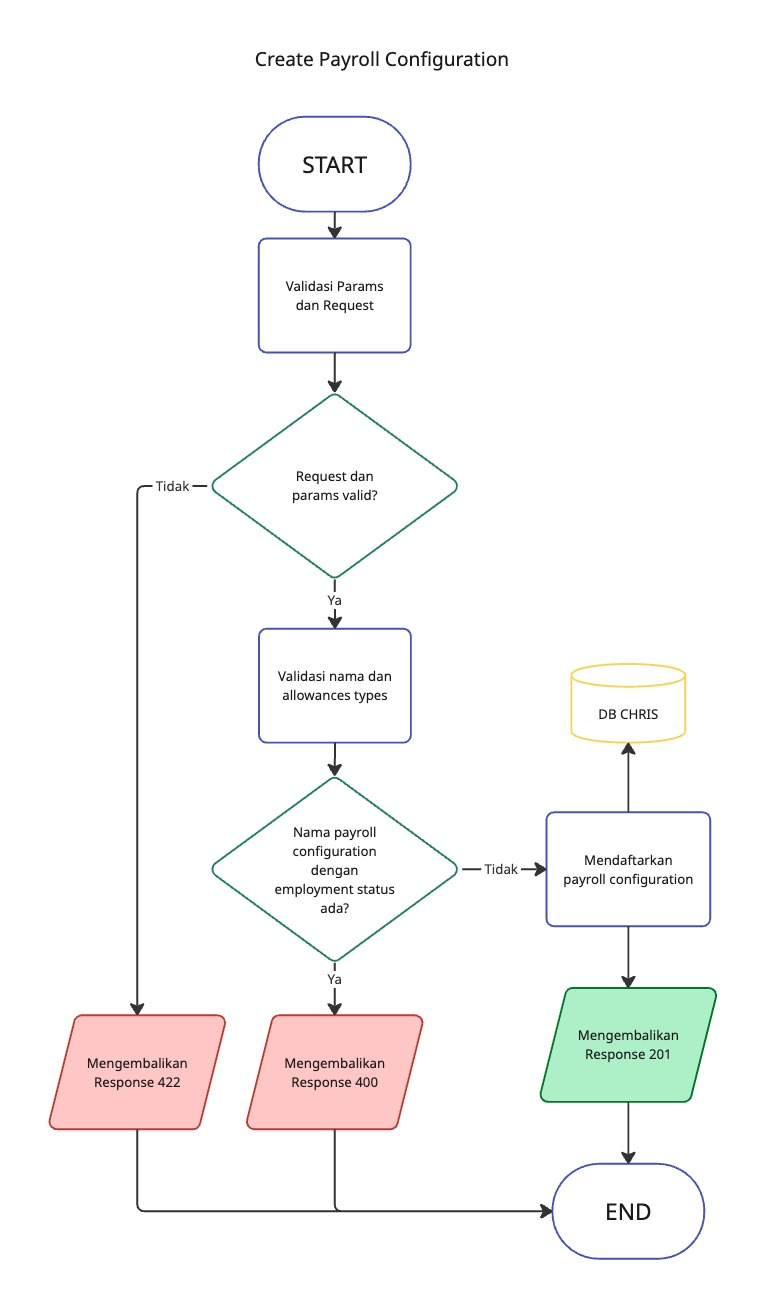
\includegraphics[width=0.8\textwidth]{assets/pics/payroll-config-create.jpg}}
    \caption{\textit{Flowchart create payroll configuration}}
    \label{fig:create_payroll_config}
\end{figure}

\begin{figure}[H]
    \centering
    \fbox{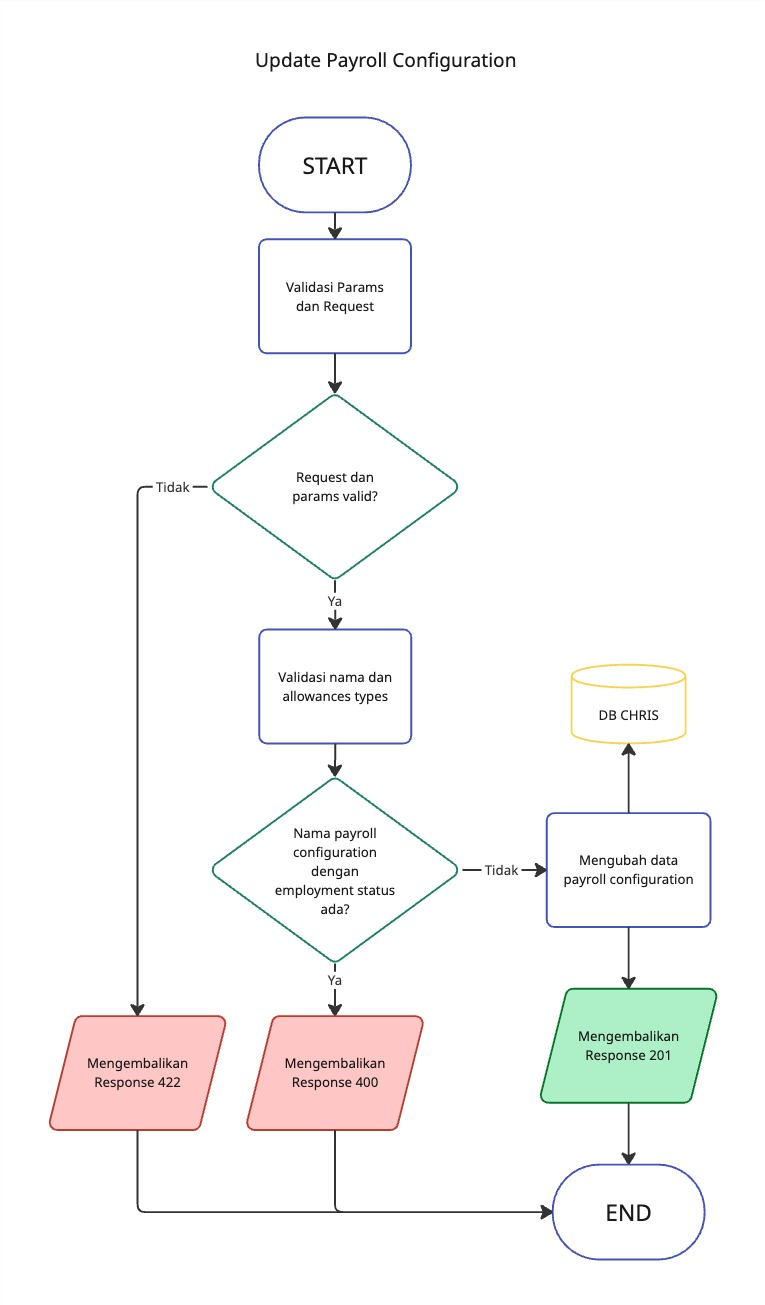
\includegraphics[width=0.8\textwidth]{assets/pics/payroll-config-update.jpg}}
    \caption{\textit{Flowchart update payroll configuration}}
    \label{fig:update_payroll_config}
\end{figure}

\begin{figure}[H]
    \centering
    \fbox{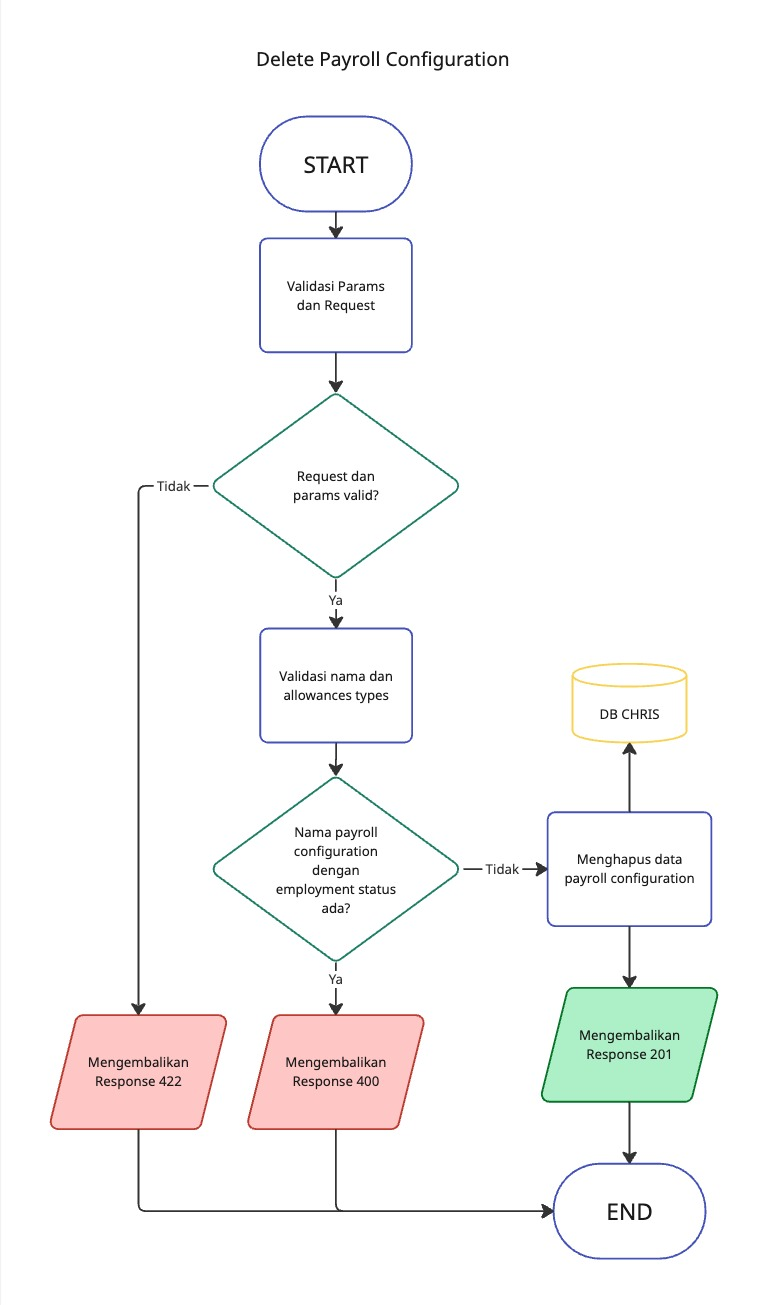
\includegraphics[width=0.8\textwidth]{assets/pics/payroll-config-delete.jpg}}
    \caption{\textit{Flowchart delete payroll configuration}}
    \label{fig:delete_payroll_config}
\end{figure}

Gambar \ref{fig:create_payroll_config}, \ref{fig:update_payroll_config}, dan \ref{fig:delete_payroll_config} menggambarkan alur proses pembuatan, pengubahan, dan penghapusan data \textit{Payroll Configuration}. Ketiga proses tersebut menerapkan validasi yang sama, yaitu pengecekan \textit{request} dan \textit{params}, dan pengecekan terhadap kombinasi nama Payroll Configuration dan Employment\textit{ Status} yang sudah terdaftar sebelumnya.

Apabila \textit{request} atau \textit{parameter} yang dikirimkan tidak sesuai dengan format atau aturan yang telah ditentukan, sistem akan merespons dengan kode 422 (\textit{Invalid Format}) sebagai penolakan terhadap permintaan yang tidak valid. Selain itu, jika kombinasi nama \textit{Payroll Configuration} dan \textit{Employment Status} telah terdaftar sebelumnya, sistem akan mengembalikan respons kode 400 (\textit{Bad Request}) untuk mencegah terjadinya duplikasi data.

Validasi ini bertujuan untuk menjaga konsistensi dan integritas data dalam sistem. Jika seluruh validasi berhasil dilewati, maka proses pembuatan, pengubahan, atau penghapusan akan dilanjutkan, dengan sistem memberikan respons berupa kode 201 (Created) untuk pembuatan, serta kode 200 (OK) untuk pengubahan dan penghapusan data.

% ----------------------%
\paragraph{User Allowances}
% ----------------------%
Setelah \textit{Superadmin} membuat \textit{payroll configuration}, langkah selanjutnya adalah mengatur data gaji setiap pegawai. Proses ini dilakukan melalui modul \textit{User Management}, di mana \textit{Superadmin} memilih \textit{Payroll Configuration} berdasarkan status kepegawaian pengguna, mengisi besaran gaji pokok, serta melengkapi jumlah masing-masing tunjangan yang ditetapkan. 

% -------------------- %
\begin{figure}[H]
    \centering
    \fbox{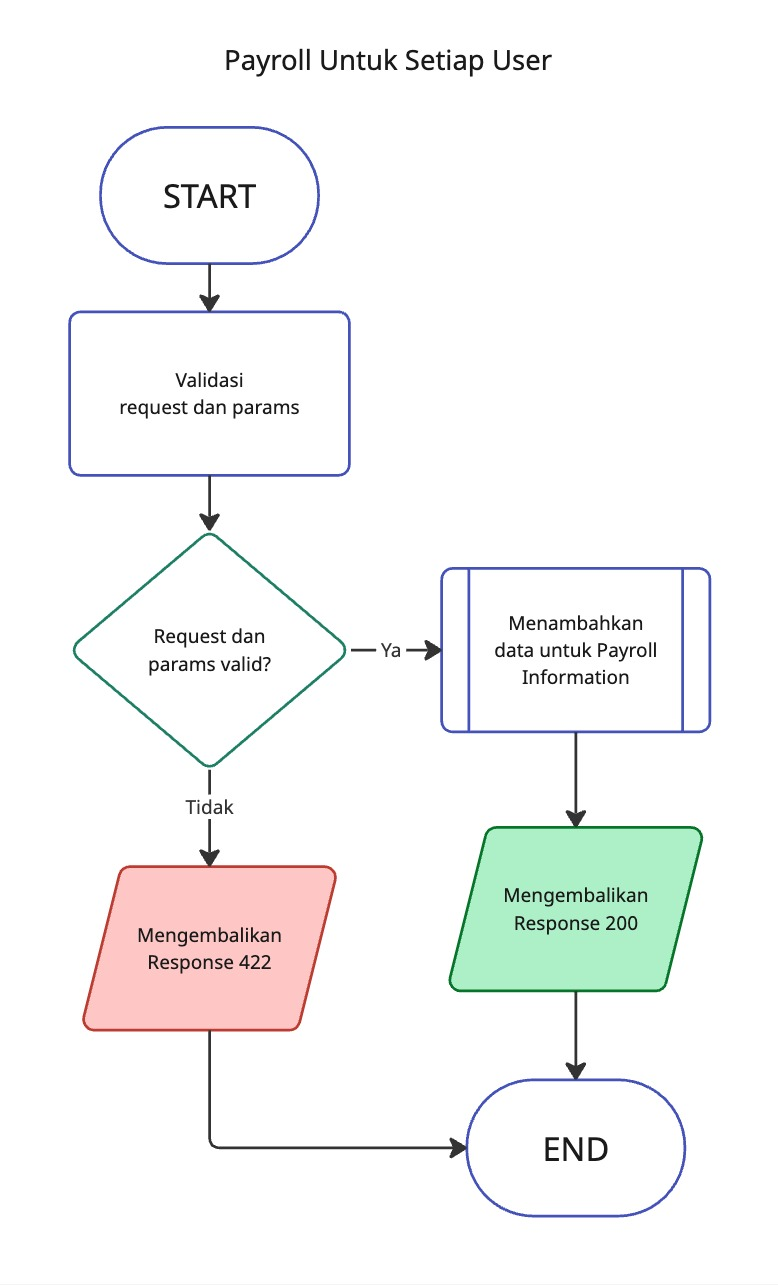
\includegraphics[height=0.7\textheight]{assets/pics/payroll-untuk-setiap-user.jpg}}
    \caption{\textit{Flowchart} implementasi payroll untuk setiap user}
    \label{fig:payroll_untuk_setiap_user}
\end{figure}

Gambar \ref{fig:payroll_untuk_setiap_user} menunjukkan proses untuk validasi \textit{request} dan \textit{parameter} akan dilanjuti dengan proses menambahkan data untuk \textit{payroll information} secara \textit{general}.

% -------------------- %
\begin{figure}[H]
    \centering
    \fbox{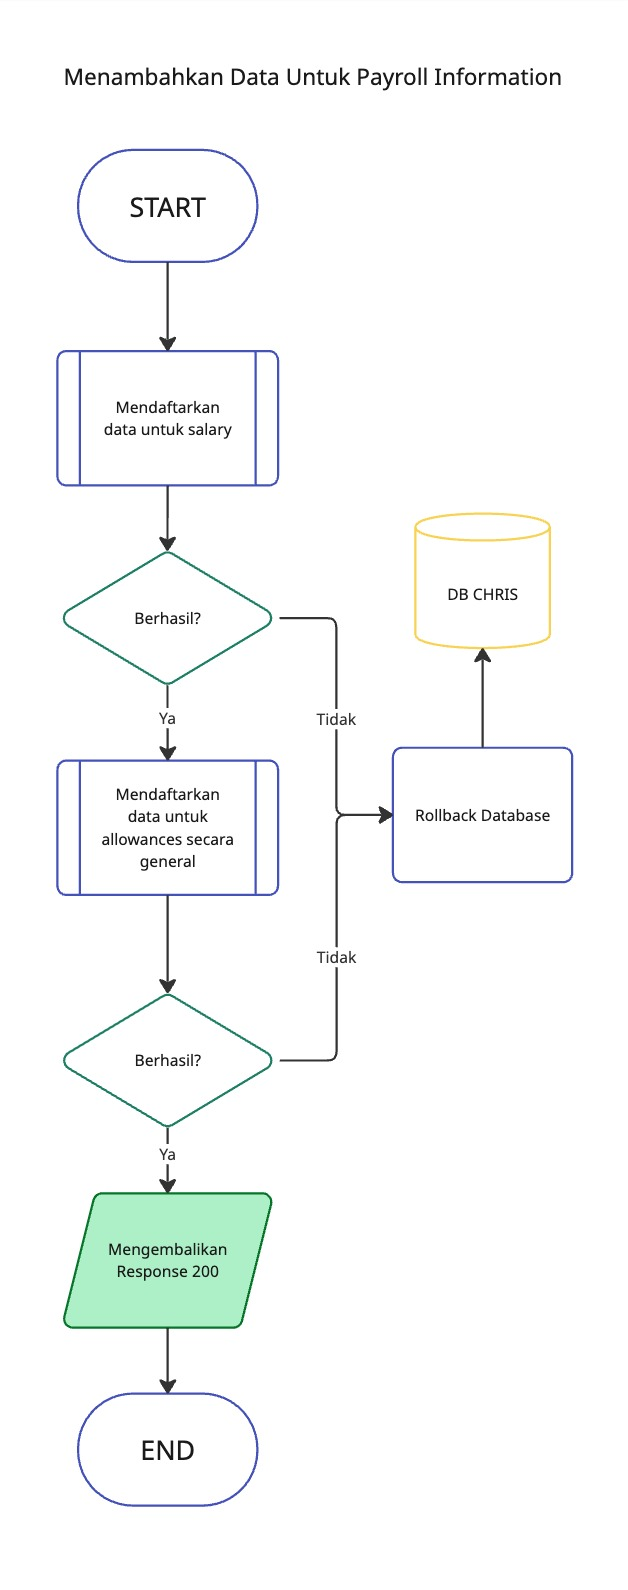
\includegraphics[height=0.7\textheight]{assets/pics/menambahkan-data-untuk-payroll-information.jpg}}
    \caption{\textit{Flowchart} menambahkan data untuk payroll information}
    \label{fig:menambahkan_data_payroll_information}
\end{figure}

Pada \textit{user management}, terdapat suatu field bernama \textit{Payroll Information} yang berisi data gaji pegawai, dan field untuk memilih \textit{Payroll Configuration} yang telah dibuat sebelumnya. Setelah memilih \textit{Payroll Configuration}, \textit{Superadmin} dapat mengisi data gaji pokok, tunjangan, dan potongan yang berlaku untuk pegawai tersebut. Gambar \ref{fig:payroll_untuk_setiap_user} menunjukkan alur sistem untuk pembuatan data gaji pegawai.

% -------------------- %
\begin{figure}[H]
    \centering
    \fbox{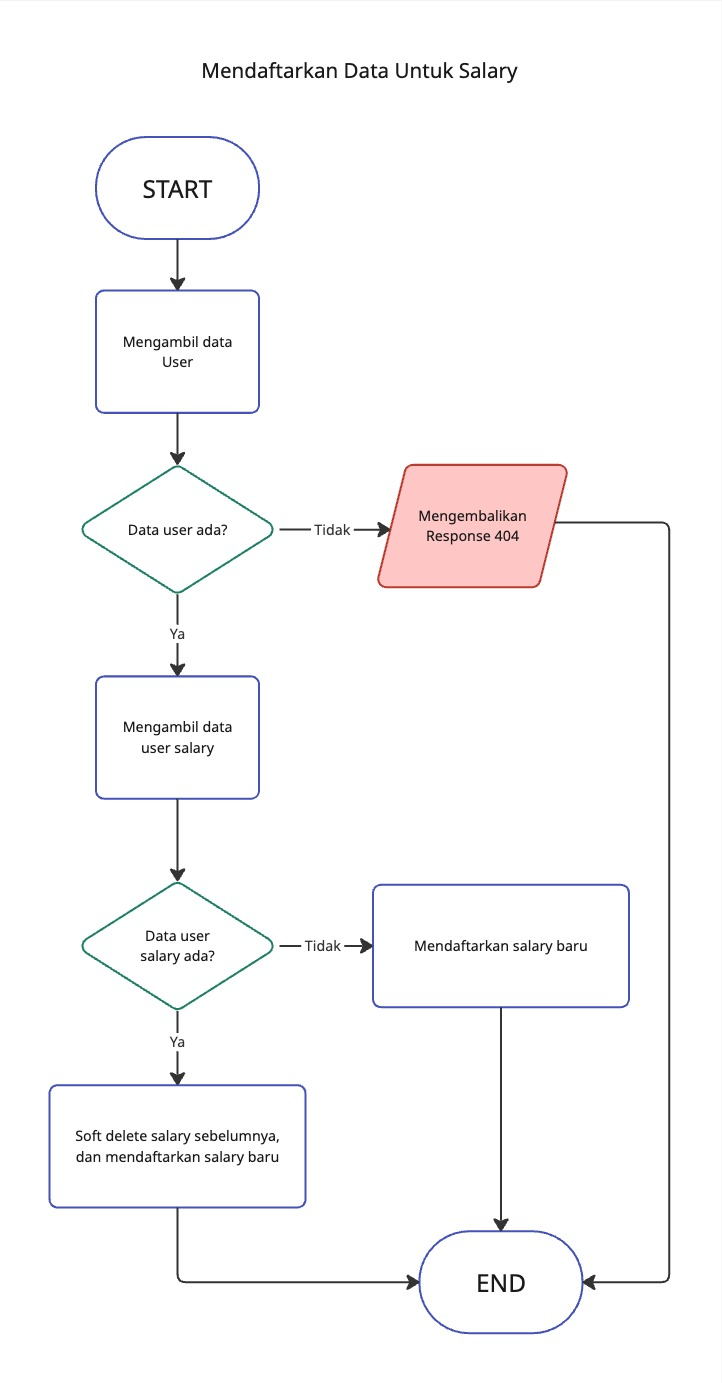
\includegraphics[height=0.7\textheight]{assets/pics/mendaftarkan-data-untuk-salary.jpg}}
    \caption{\textit{Flowchart} mendaftarkan data untuk salary}
    \label{fig:mendaftarkan_data_untuk_salary}
\end{figure}

Gambar \ref{fig:mendaftarkan_data_untuk_salary} menunjukkan proses pembuatan data gaji pegawai yang dimulai dengan mencari data pegawai dan mengambil data gaji pegawai tersebut. Setelah itu, jika data tersebut ditemukan, sistem akan menghapus data gaji pegawai yang lama secara \textit{soft delete} dan membuat data gaji pegawai yang baru.
% -------------------- %
\begin{figure}[H]
    \centering
    \fbox{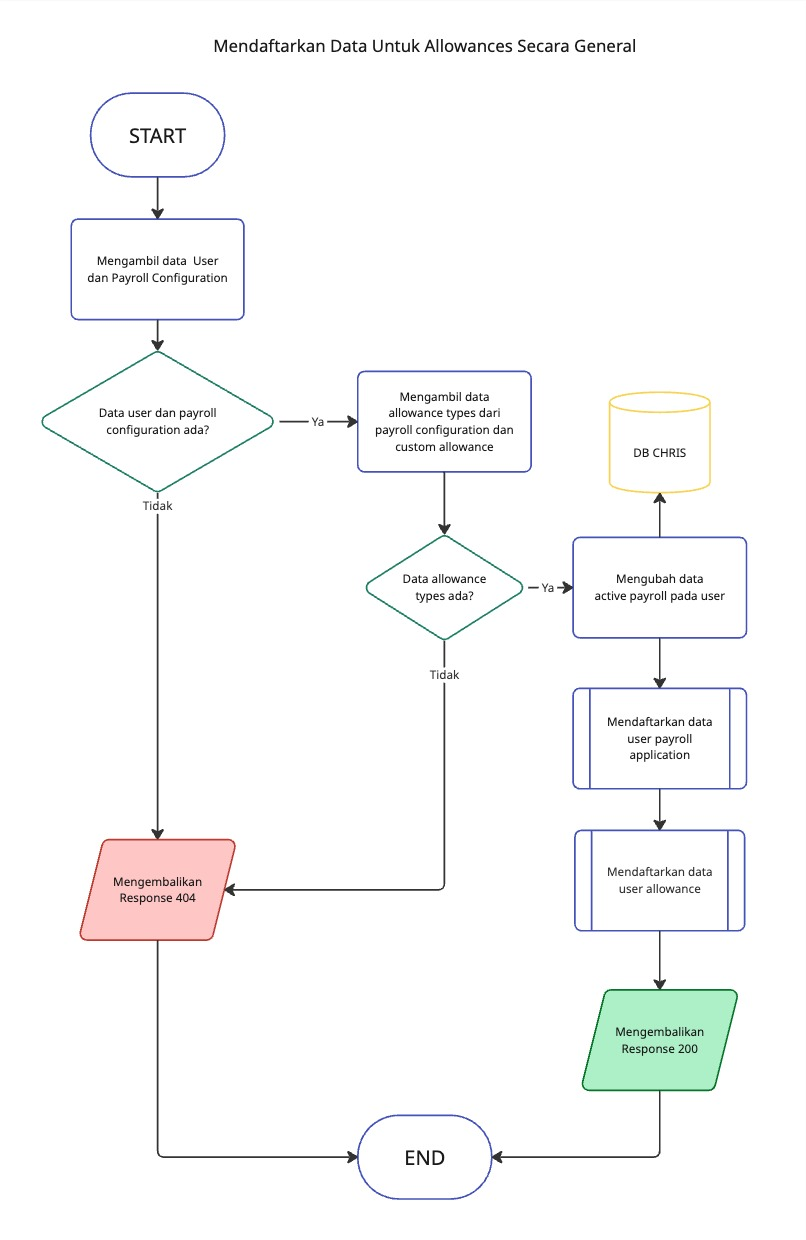
\includegraphics[height=0.6\textheight]{assets/pics/mendaftarkan-data-untuk-allowances-secara-general.jpg}}
    \caption{\textit{Flowchart} mendaftarkan data user allowances secara \textit{general}}
    \label{fig:mendaftarkan_data_user_allowances_secara_general}
\end{figure}

Gambar \ref{fig:mendaftarkan_data_user_allowances_secara_general} menggambarkan alur proses pendaftaran data tunjangan pegawai secara umum. Proses ini diawali dengan pengambilan data pegawai dan \textit{Payroll Configuration} yang telah tersedia. Selanjutnya, sistem mengekstraksi daftar tunjangan yang tercantum dalam \textit{Payroll Configuration} tersebut. Setelah itu, sistem akan memperbarui informasi \textit{Active Payroll} pada data pegawai, dan mendaftarkan entri baru pada \textit{User Payroll Application} guna menghubungkan pegawai dengan konfigurasi payroll yang aktif. Terakhir, sistem akan mendaftarkan data \textit{User Allowances} beserta nominal masing-masing tunjangan dan potongan yang telah ditentukan sebelumnya.

% -------------------- %
\begin{figure}[H]
    \centering
    \fbox{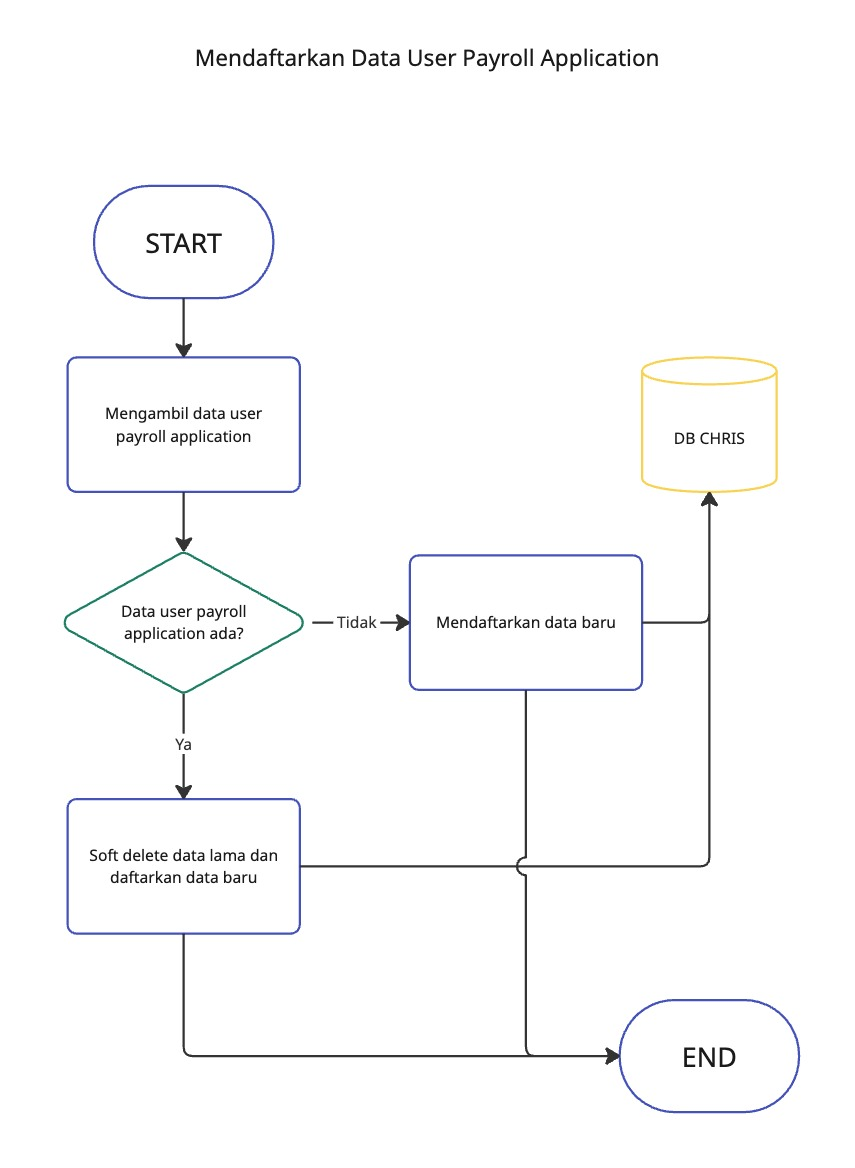
\includegraphics[height=0.8\textheight]{assets/pics/mendaftarkan-data-user-payroll-application.jpg}}
    \caption{\textit{Flowchart} mendaftarkan data \textit{user payroll application}}
    \label{fig:mendaftarkan_data_user_payroll_application}
\end{figure}

Gambar \ref{fig:mendaftarkan_data_user_payroll_application} menggambarkan proses pendaftaran data \textit{User Payroll Application} yang diawali dengan pencarian entri sebelumnya pada pegawai terkait. Jika tidak ditemukan, sistem akan langsung membuat entri baru pada tabel \textit{User Payroll Application}. Namun, apabila entri sudah ada, sistem akan terlebih dahulu melakukan \textit{soft delete} terhadap data tersebut, kemudian membuat entri baru guna memastikan hanya satu konfigurasi aktif yang tercatat untuk setiap pegawai. Pendekatan ini menjaga integritas historis tanpa menghapus data secara permanen.


% -------------------- %
\begin{figure}[H]
    \centering
    \fbox{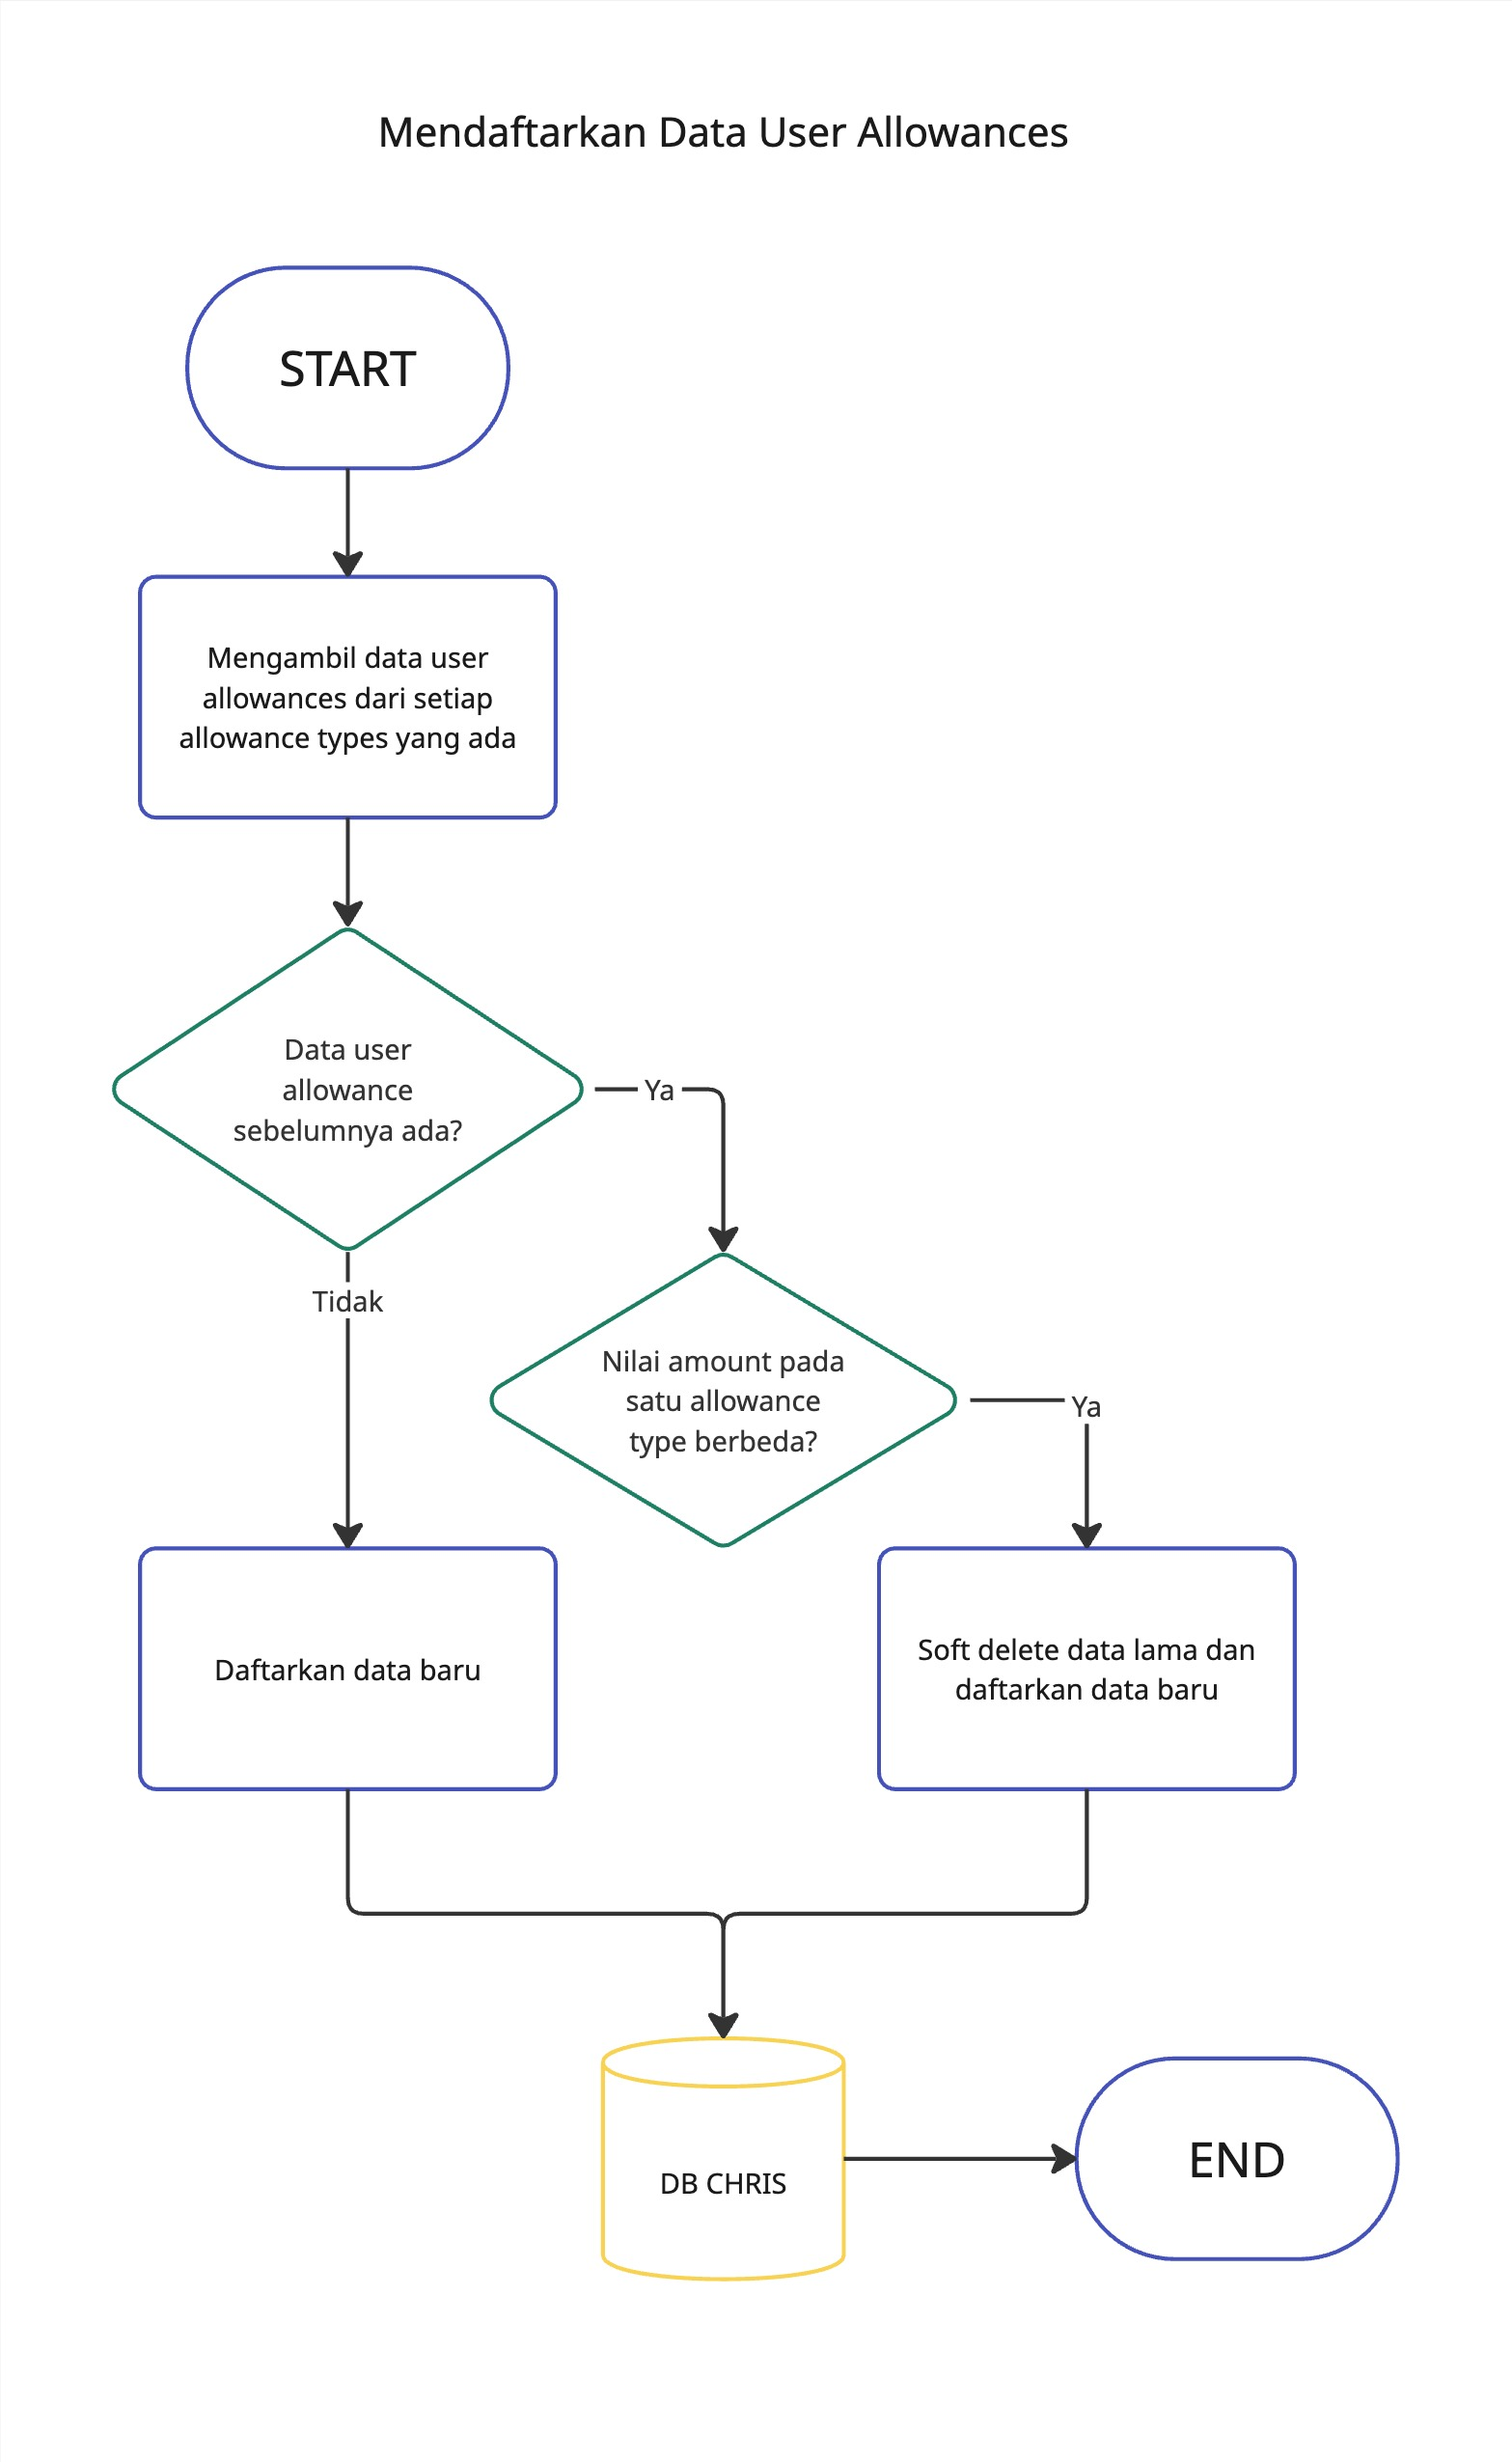
\includegraphics[height=0.7\textheight]{assets/pics/mendaftarkan-data-user-allowances.jpg}}
    \caption{\textit{Flowchart} mendaftarkan data \textit{user allowances}}
    \label{fig:mendaftarkan_data_user_allowances}
\end{figure}

Gambar \ref{fig:mendaftarkan_data_user_allowances} menggambarkan proses pendaftaran data tunjangan pegawai yang diawali dengan pencarian data \textit{User Allowances} berdasarkan setiap \textit{Allowance Type} yang dimiliki pegawai. Apabila data tidak ditemukan, sistem akan membuat entri baru dengan mengisikan \textit{Allowance Type} beserta nominal tunjangan yang telah ditentukan. Namun, jika data ditemukan, sistem akan melakukan pengecekan terhadap kesesuaian nominal tunjangan. Jika nominal yang ditemukan sama, maka tidak ada perubahan yang dilakukan. Sebaliknya, jika terdapat perbedaan, sistem akan memperbarui nilai nominal dengan yang baru, serta melakukan \textit{soft delete} pada data lama. Pendekatan ini diterapkan untuk menjaga riwayat data dan memungkinkan pelacakan perubahan secara historis.

% -------------------- %
% SALARY SLIP
\paragraph{Salary Slip}
% -------------------- %
Setelah data gaji pegawai selesai dibuat, \textit{Superadmin} dapat mengakses modul \textit{Salary Slip} untuk melakukan finalisasi gaji. Proses finalisasi ini memungkinkan pengecekan akhir terhadap rincian gaji sebelum tanggal gajian. Di PT Ganda Visi Jayatama, proses penggajian dilakukan setiap tanggal 25, sehingga proses finalisasi disarankan dilakukan pada tanggal 24 setiap bulannya. Setelah tanggal 25, data tidak dapat lagi diubah.
\begin{figure}[H]
    \centering
    \fbox{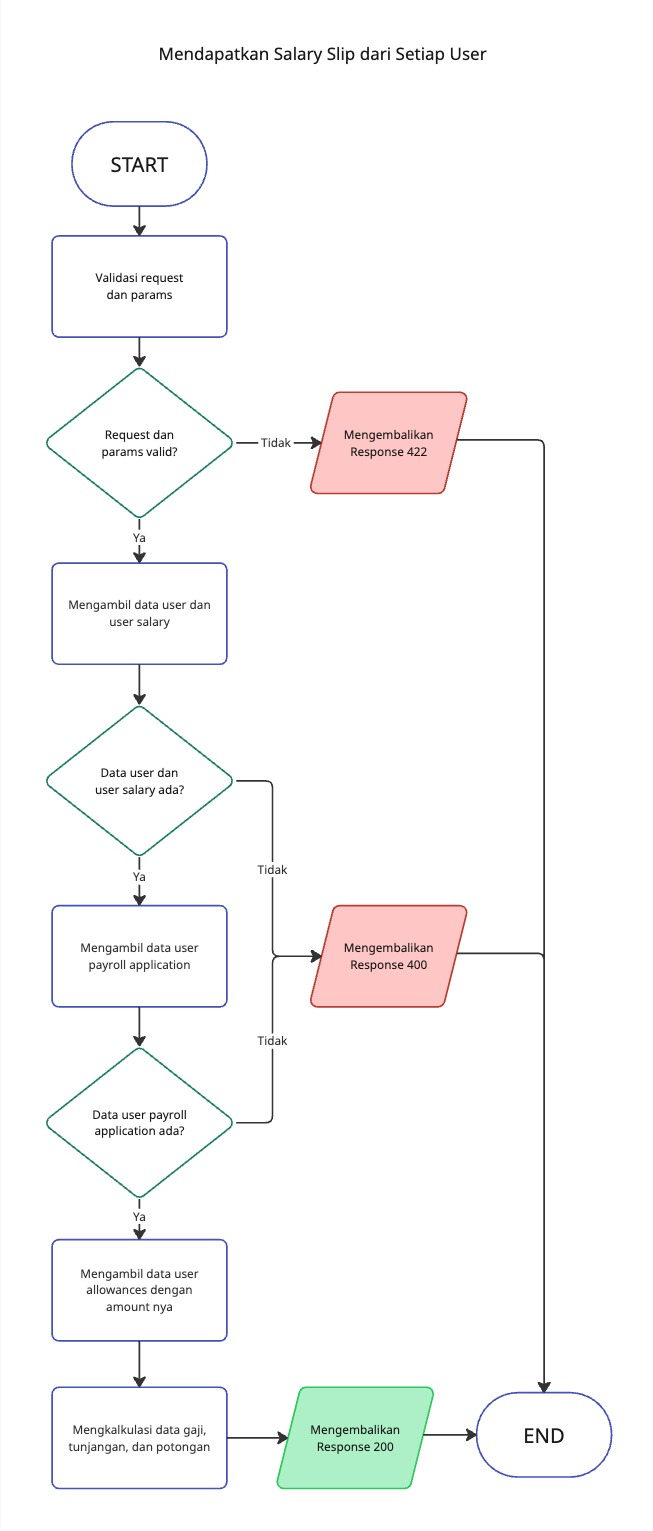
\includegraphics[height=0.8\textheight]{assets/pics/mendapatkan-salary-slip-dari-setiap-user.jpg}}
    \caption{\textit{Flowchart} mendapatkan salary slip dari setiap user}
    \label{fig:mendapatkan_salary_slip_dari_setiap_user}
\end{figure}

Gambar \ref{fig:mendapatkan_salary_slip_dari_setiap_user} menunjukkan proses mendapatkan slip gaji pegawai yang dimulai dengan mencari data pegawai berdasarkan \textit{Payroll Configuration} yang telah dibuat sebelumnya. Setelah itu, sistem akan mengambil data gaji pegawai, tunjangan-tunjangan yang telah dibuatkan sebelumnya, dan membuat slip gaji berdasarkan data tersebut. 

Untuk pegawai yang telah memiliki data gaji terverifikasi, mereka dapat melihat slip gaji mereka masing-masing pada halaman \textit{Salary Slip} dan mengunduhnya dalam format PDF. Hal ini memungkinkan pegawai untuk mengakses informasi gaji mereka secara transparan dan mudah.

Untuk mendapatkan slip gaji historis, sistem akan terlebih dahulu menentukan periode waktu berdasarkan tanggal yang diminta, yaitu awal hingga akhir bulan tersebut. Setelah itu, sistem akan mencari seluruh entri data gaji (\textit{User Salary}) yang memiliki tanggal pembuatan (\textit{created\_at}) sebelum atau sama dengan akhir periode, dan belum dihapus atau dihapus setelah periode tersebut berakhir. Seluruh data yang ditemukan kemudian diurutkan berdasarkan tanggal pembuatan dari yang terbaru ke yang terlama. Dari hasil pengurutan tersebut, sistem akan memilih satu entri data gaji paling terbaru yang masih berlaku pada periode tersebut. Entri tersebut kemudian digunakan untuk mengambil informasi tunjangan (\textit{User Allowances}) dan pemotongan berdasarkan konfigurasi yang berlaku, lalu disusun menjadi slip gaji pegawai.

% ---------------------------------- %
% ---------------------------------- %
\section{Implementasi Sistem}
% ---------------------------------- %
Implementasi sistem menghasilkan ... \textit{endpoint API} yang mendukung fungsionalitas dari berbagai modul yang dikembangkan. \textit{Endpoint-endpoint} ini menggunakan lima jenis metode HTTP, yaitu \textit{GET}, \textit{POST}, \textit{PUT}, \textit{DELETE}, dan \textit{PATCH}. Metode \textit{GET} digunakan untuk mengambil data dari server, sementara \textit{POST} digunakan untuk menambahkan data baru ke dalam basis data. \textit{PUT} berfungsi untuk memperbarui seluruh entri data yang ada, sedangkan \textit{PATCH} digunakan ketika hanya sebagian data yang perlu diubah. Metode {DELETE} digunakan untuk menghapus data dari sistem.

Setiap API memiliki standar struktur \textit{request} dan \textit{response} yang wajib diterapkan. Pada \textit{request}, data identifikasi dikirim melalui parameter kueri (\textit{query params}). Untuk \textit{response}, format yang digunakan harus mencakup tiga elemen utama, yaitu \textit{code} (kode status), \textit{message} (pesan status), dan \textit{data} (isi data). Contoh implementasi struktur \textit{request} dan \textit{response} dapat dilihat pada gambar yang disediakan.


\subsection{Implementasi \textit{User Management} dan Validasi Data}
\subsubsection{API \textit{Endpoints}}
Berikut adalah daftar \textit{endpoint} yang telah dimodifikasi dan ditambahkan untuk modul \textit{User Management}:


\begin{center}
    \begin{longtable}{|c|p{0.3\textwidth}|c|p{0.4\textwidth}|}
    \caption{\textit{User Management} API \textit{Endpoints}} 
    \label{tab:tbl_user_management_endpoints} \\
    \hline
    \textbf{No.} & \textbf{Endpoint} & \textbf{Method} & \textbf{Deskripsi Singkat} \\
    \hline
    \endfirsthead

    \multicolumn{4}{c}%
    {{\tablename\ \thetable{} \textit{User Management} API \textit{Endpoints} (lanjutan)}} \\
    \hline
    \textbf{No.} & \textbf{Endpoint} & \textbf{Method} & \textbf{Deskripsi Singkat} \\
    \hline
    \endhead

    \hline 
    \multicolumn{4}{|r|}{{Lanjut di halaman berikutnya}} \\
    \hline
    \endfoot

    \hline
    \endlastfoot

    1 & \texttt{/auth/register} & POST & Membuat entri data pegawai baru untuk menggunakan sistem CHRIS. \\ \hline
    2 & \texttt{/users/update} & PATCH & Mengubah data pegawai yang sudah ada sebelumnya. \\ \hline
    3 & \texttt{/employee-statuses} & GET & Mengambil daftar semua jenis kepegawaian (\textit{employment status}). \\ \hline
    4 & \texttt{/banks} & GET & Mengambil daftar semua jenis bank . \\ \hline

    \end{longtable}
\end{center}

Pada Tabel \ref{tab:tbl_user_management_endpoints}, ditampilkan sejumlah endpoint yang telah ditambahkan dan dimodifikasi untuk modul \textit{User Management}. Setiap \textit{endpoint} dilengkapi dengan metode HTTP yang sesuai dengan tujuannya: \textit{POST} digunakan untuk pembuatan data baru, \textit{PATCH} untuk pembaruan data, dan \textit{GET} untuk pengambilan data dari basis data.

Secara khusus, \textit{endpoint} seperti \texttt{/users/register} dan \texttt{/users/update} memiliki proses validasi input untuk memastikan data yang masuk telah memenuhi format dan ketentuan yang berlaku. \textit{Field} yang divalidasi ulang meliputi:
\begin{itemize}
    \item \textit{fullname}: Nama lengkap pegawai, wajib diisi dan harus berupa karakter alfanumerik yang valid.
    \item \textit{email}: Alamat \textit{email} pegawai, Hanya menerima domain @concise.co.id dengan format yang sesuai menggunakan ekspresi reguler dan wajib diisi.
    \item \textit{nik}: Nomor Induk Kependudukan pegawai, Wajib 16 digit angka.
    \item \textit{contact} dan \textit{emergency\_contact}: Nomor telepon dan nomor telepon darurat, wajib diisi dan hanya menerima nomor dengan awalan +62 atau 0.
    \item \textit{bank\_holder}: Nama terdaftar pada bank, wajib diisi dan harus alfanumerik.
    \item \textit{bank\_number}: Nomor rekening bank pegawai, wajib diisi dan hanya angka.
\end{itemize}

Validasi dilakukan untuk memastikan integritas data dan menghindari kesalahan yang dapat terjadi dalam pengolahan data pegawai, termasuk proses penggajian dan pelacakan informasi.

Sementara itu, beberapa \textit{endpoint} seperti \texttt{/employee-statuses} dan \texttt{/banks} hanya berfungsi untuk mengambil data dari basis data dan tidak melalui proses validasi karena semata-mata digunakan untuk mengisi data pendukung pada \textit{dropdown} dalam formulir pendaftaran atau pembaruan data pegawai.


\subsubsection{\textit{Request} dan \textit{Response}}
Berikut adalah struktur \textit{request} dan \textit{response} untuk \textit{endpoint} \texttt{/auth/register} pada modul \textit{User Management}:
\begin{figure}
    \centering
    \fbox{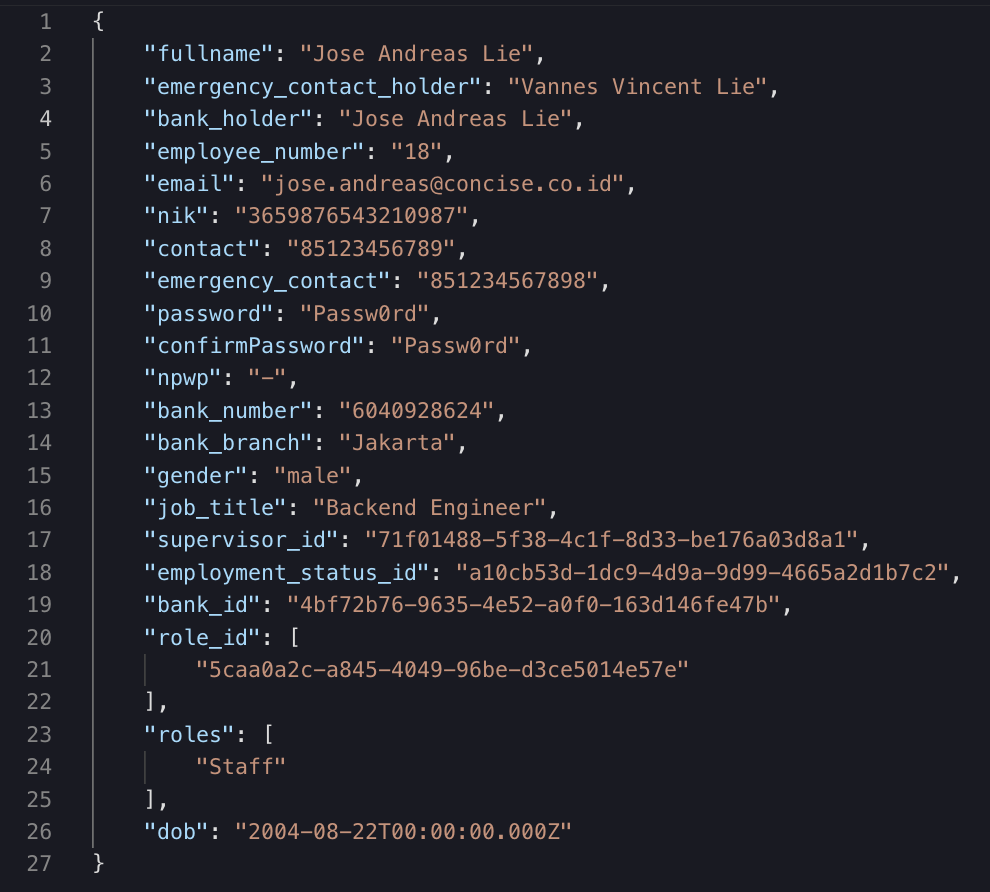
\includegraphics[width=0.8\textwidth]{assets/pics/fig_request_register_user.png}}
    \caption{Contoh struktur \textit{request} untuk \texttt{/auth/register}}
    \label{fig:request_register_user}
\end{figure}

\begin{figure}
    \centering
    \fbox{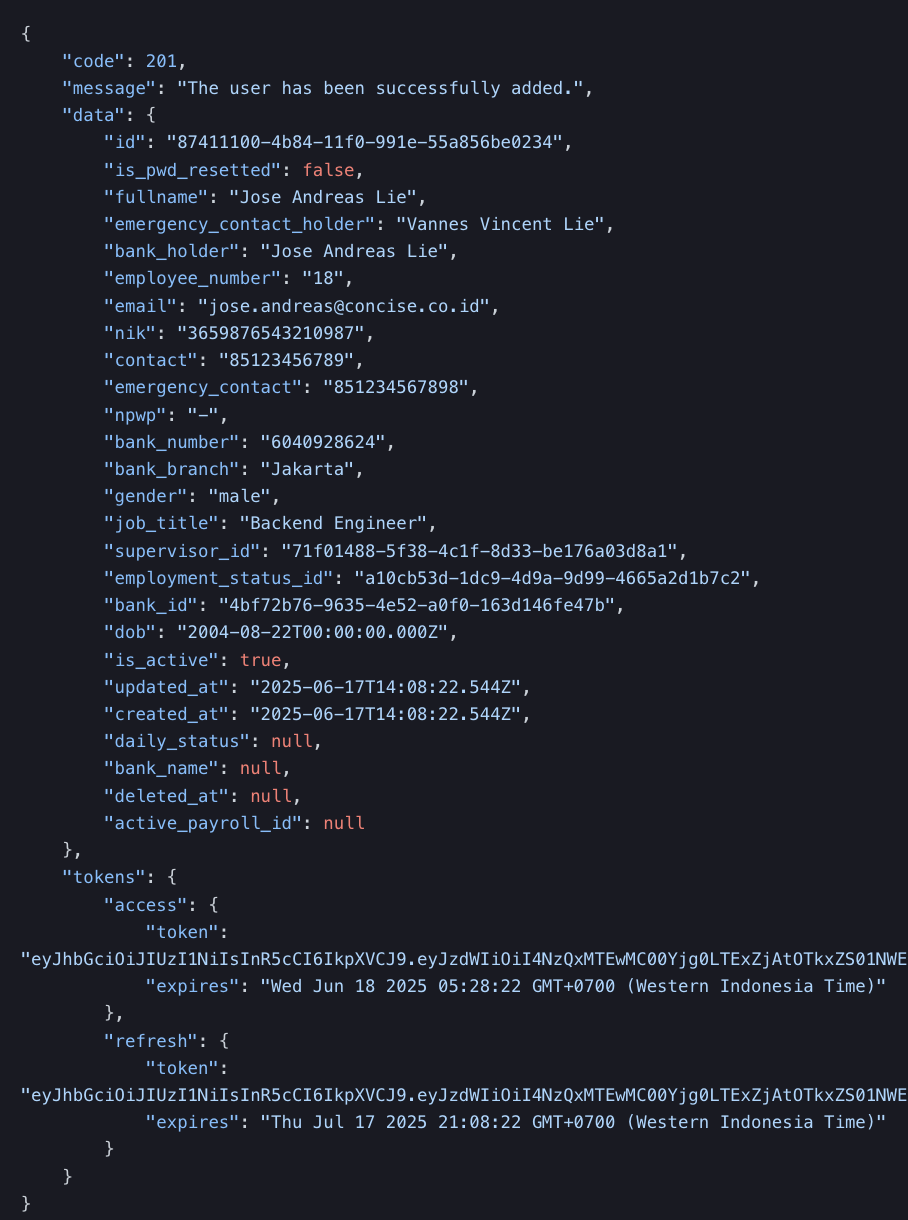
\includegraphics[width=0.8\textwidth]{assets/pics/fig_response_register_user.png}}
    \caption{Contoh struktur \textit{response} untuk \texttt{/auth/register}}
    \label{fig:response_register_user}
\end{figure}

Berikut adalah struktur \textit{request} dan \textit{response} untuk \textit{endpoint} \texttt{/users/update} pada modul \textit{User Management}:
\begin{figure}
    \centering
    \fbox{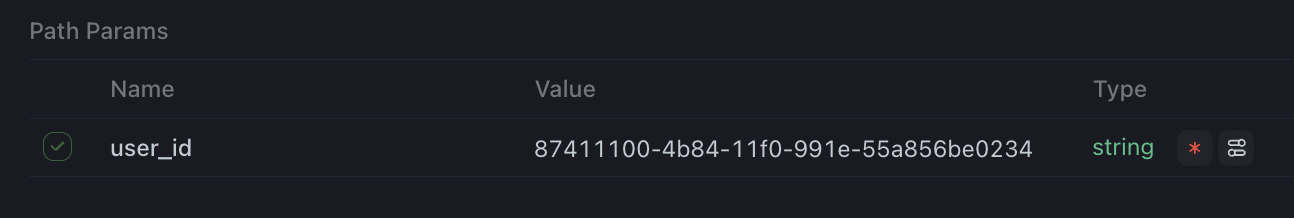
\includegraphics[width=0.8\textwidth]{assets/pics/fig_request_update_user_params.png}}
    \caption{Contoh struktur \textit{parameters} untuk \texttt{/users/update}}
    \label{fig:request_update_user_params}
\end{figure}
\begin{figure}
    \centering
    \fbox{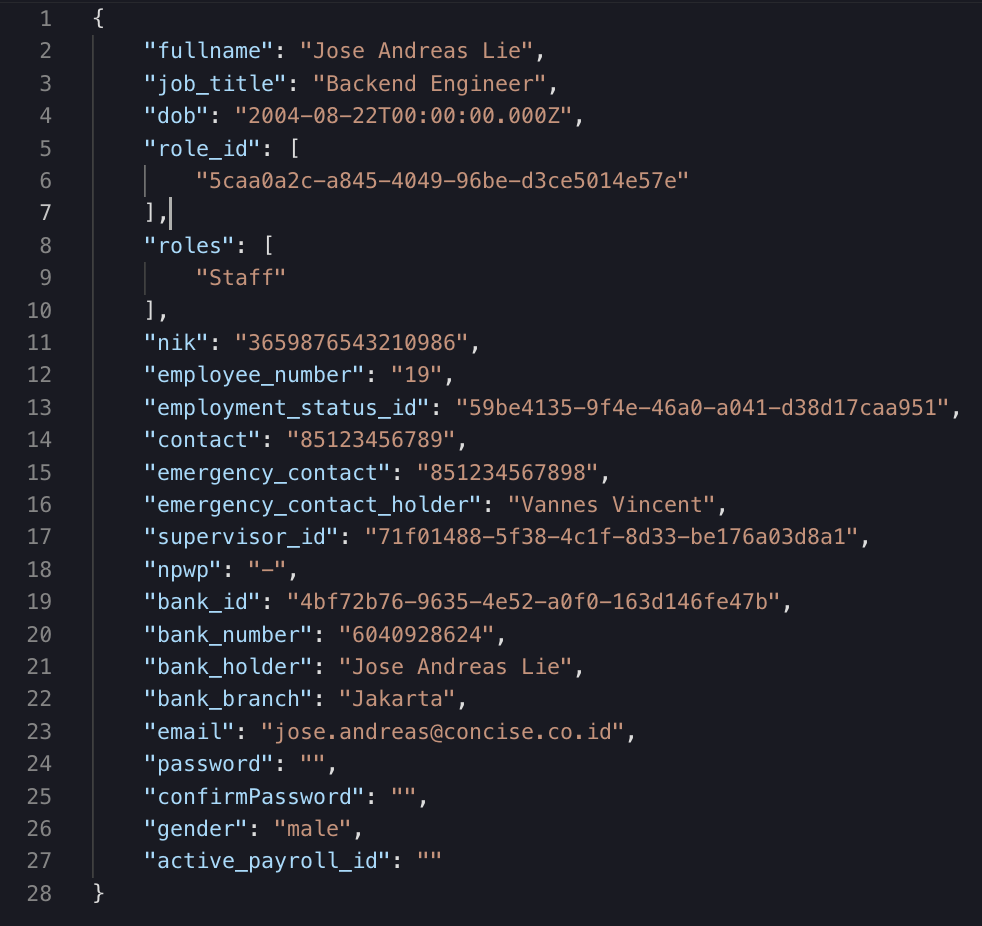
\includegraphics[width=0.8\textwidth]{assets/pics/fig_request_update_user.png}}
    \caption{Contoh struktur \textit{request} untuk \texttt{/users/update}}
    \label{fig:request_update_user}
\end{figure}

\begin{figure}
    \centering
    \fbox{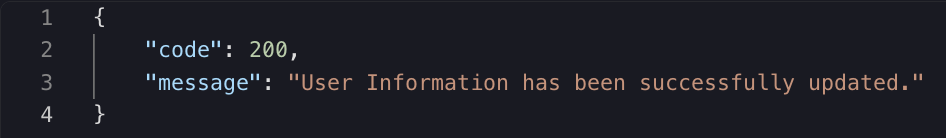
\includegraphics[width=0.8\textwidth]{assets/pics/fig_response_update_user.png}}
    \caption{Contoh struktur \textit{response} untuk \texttt{/users/update}}
    \label{fig:response_update_user}
\end{figure}


Pada gambar \ref{fig:request_register_user}, terlihat struktur \textit{request} yang dikirimkan ke \textit{endpoint} \texttt{/auth/register}. Data yang dikirim mencakup informasi pegawai seperti nama lengkap, alamat email, nomor induk kependudukan (NIK), nomor telepon, kontak darurat, nama pemegang rekening bank, nomor rekening bank, dan masih banyak lagi. Setelah request berhasil diproses, sistem akan mengembalikan respons seperti pada gambar \ref{fig:response_register_user}, yang menunjukkan bahwa pendaftaran pegawai baru berhasil dengan kode status 201 (Created) dan pesan yang sesuai.

Pada gambar \ref{fig:request_update_user_params} dan \ref{fig:request_update_user}, terlihat struktur \textit{request} yang dikirimkan ke \textit{endpoint} \texttt{/users/update}. Data yang dikirim sama seperti yang dikirim pada \textit{request} pendaftaran, namun dengan tambahan \textit{id} pegawai yang akan diperbarui pada bagian parameter. Setelah \textit{request} berhasil diproses, sistem akan mengembalikan respons seperti pada gambar \ref{fig:response_update_user}, yang menunjukkan bahwa pembaruan data pegawai berhasil dengan kode status 200 (OK) dan pesan yang sesuai.

% ------------------------- %
Berikut adalah struktur \textit{response} untuk \textit{endpoint} \texttt{/employee-statuses} pada modul \textit{User Management}:
\begin{figure}
    \centering
    \fbox{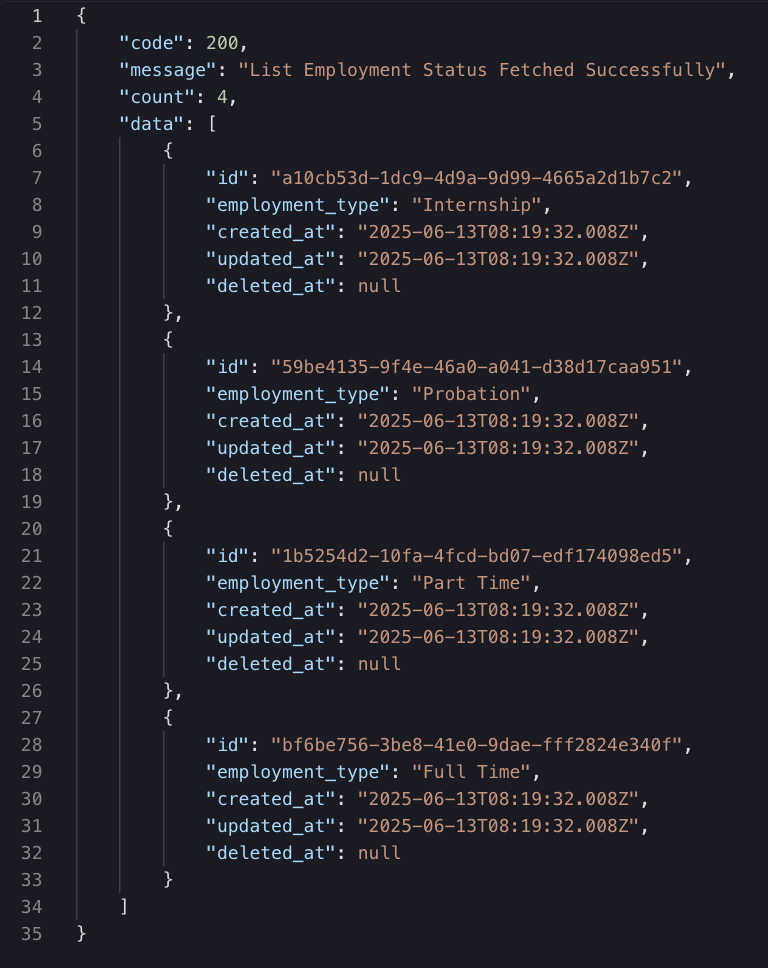
\includegraphics[width=0.8\textwidth]{assets/pics/fig_response_employee_statuses.png}}
    \caption{Contoh struktur \textit{request} untuk \texttt{/employee-statuses}}
    \label{fig:request_employee_statuses}
\end{figure}

Berikut adalah struktur \textit{response} untuk \textit{endpoint} \texttt{/banks} pada modul \textit{User Management}:
\begin{figure}
    \centering
    \fbox{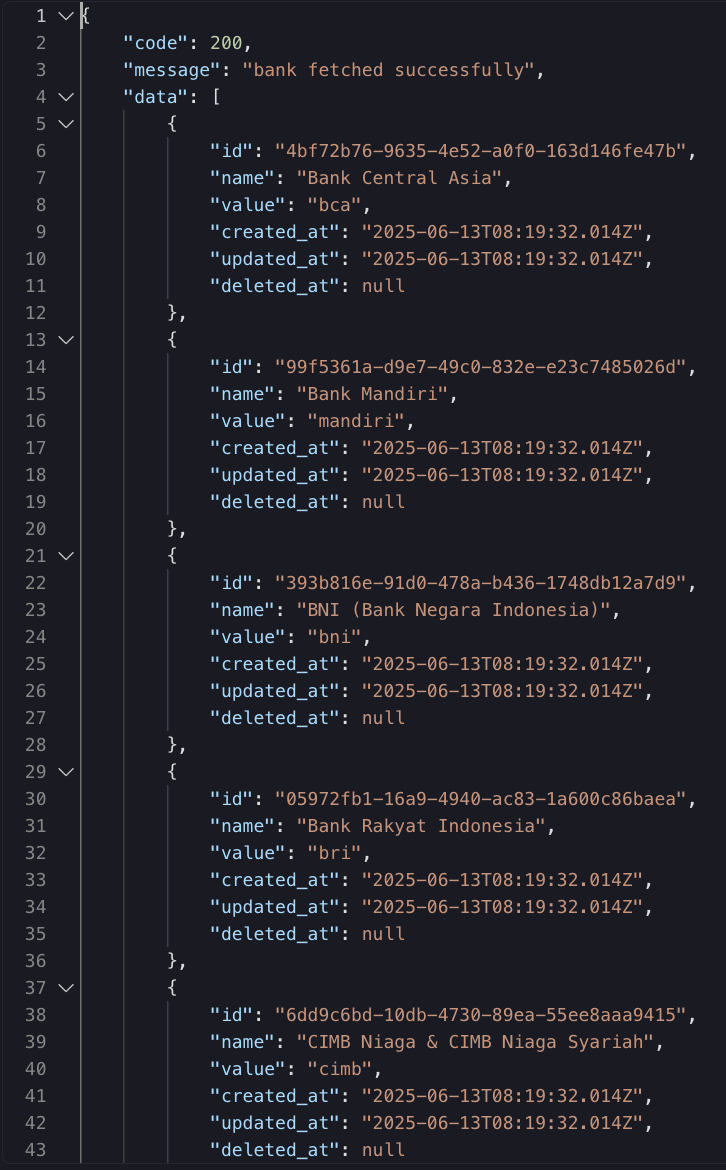
\includegraphics[width=0.8\textwidth]{assets/pics/fig_response_banks.png}}
    \caption{Contoh struktur \textit{request} untuk \texttt{/banks}}
    \label{fig:request_banks}
\end{figure}



\subsection{Implementasi Fitur Autentikasi Biometrik pada CHRIS \textit{Mobile}}
\subsubsection{API \textit{Endpoints}}
Berikut adalah daftar \textit{endpoint} yang telah ditambahkan untuk fitur autentikasi biometrik pada CHRIS \textit{Mobile}:
\begin{center}
    \begin{longtable}{|c|p{0.37\textwidth}|c|p{0.33\textwidth}|}
    \caption{\textit{Biometric Authentication} API \textit{Endpoints}} 
    \label{tab:tbl_biometric_authentication_endpoints} \\
    \hline
    \textbf{No.} & \textbf{Endpoint} & \textbf{Method} & \textbf{Deskripsi Singkat} \\
    \hline
    \endfirsthead

    \multicolumn{4}{c}%
    {{\tablename\ \thetable{} -- lanjutan}} \\
    \hline
    \textbf{No.} & \textbf{Endpoint} & \textbf{Method} & \textbf{Deskripsi Singkat} \\
    \hline
    \endhead

    \hline 
    \multicolumn{4}{|r|}{{Lanjut di halaman berikutnya}} \\
    \hline
    \endfoot

    \hline
    \endlastfoot

    1 & \texttt{/auth/biometric/register} & POST & Mendaftarkan data biometrik pegawai baru untuk autentikasi. \\ \hline
    2 & \texttt{/auth/biometric/login} & POST & Melakukan autentikasi pegawai menggunakan data biometrik yang telah didaftarkan. \\

    \end{longtable}
\end{center}
Pada Tabel \ref{tab:tbl_biometric_authentication_endpoints}, ditampilkan daftar \textit{endpoint} yang telah ditambahkan untuk fitur autentikasi biometrik pada CHRIS \textit{Mobile}. Setiap \textit{endpoint} dilengkapi dengan metode HTTP yang sesuai dengan tujuannya: \textit{POST} digunakan untuk pendaftaran data biometrik pegawai baru dan autentikasi pegawai menggunakan data biometrik yang telah didaftarkan.

\subsubsection{Contoh \textit{Request} dan \textit{Response}}
\begin{figure}
    \centering
    \fbox{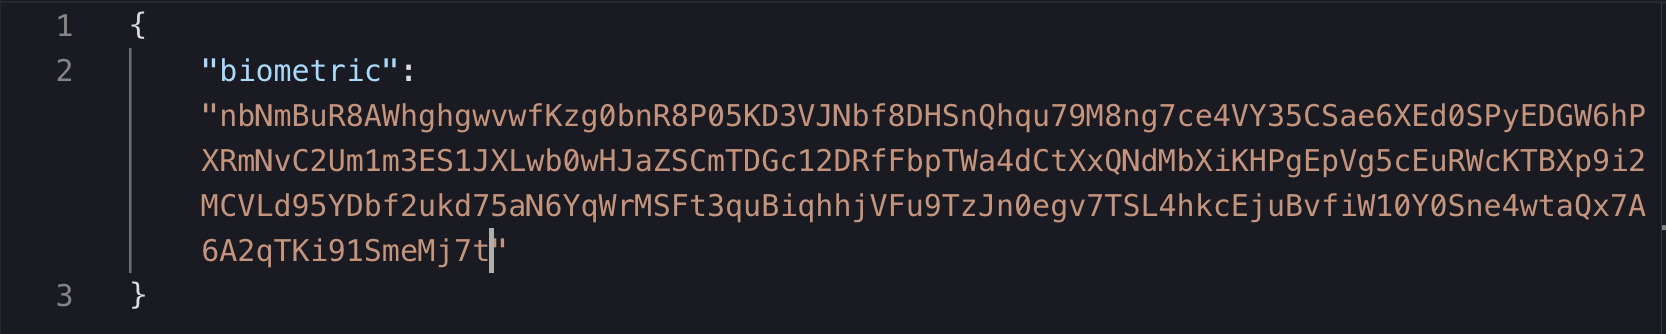
\includegraphics[width=0.8\textwidth]{assets/pics/fig_request_biometric_register.png}}
    \caption{Contoh struktur \textit{request} untuk \texttt{/auth/biometric/register}}
    \label{fig:request_biometric_register}
\end{figure}

\begin{figure}
    \centering
    \fbox{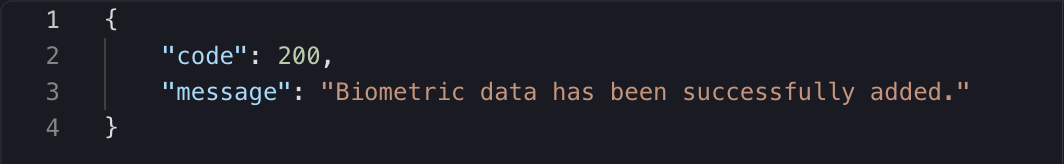
\includegraphics[width=0.8\textwidth]{assets/pics/fig_response_biometric_register.png}}
    \caption{Contoh struktur \textit{response} untuk \texttt{/auth/biometric/register}}
    \label{fig:response_biometric_register}
\end{figure}

Pada gambar \ref{fig:request_biometric_register}, terlihat struktur \textit{request} yang dikirimkan ke \textit{endpoint} \texttt{/auth/biometric/register}. Data yang dikirim berupa nilai \textit{biometric} yang berisi string acak sepanjang 255 karakter yang dihasilkan oleh aplikasi CHRISM dan akan disimpan pada penyimpanan lokal perangkat. String ini berfungsi sebagai representasi dari data biometrik pengguna, bukan data biometrik aktual yang dikirim ke server. Setelah \textit{request} berhasil diproses, sistem akan mengembalikan respons seperti pada gambar \ref{fig:response_biometric_register}, yang menunjukkan bahwa pendaftaran data biometrik pegawai berhasil dengan kode status 201 (\textit{Created}) dan pesan yang sesuai.
\begin{figure}
    \centering
    \fbox{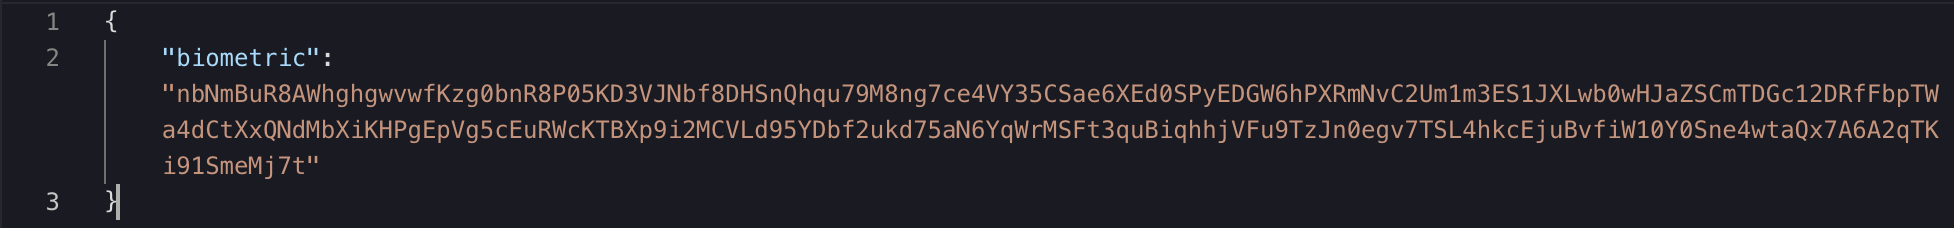
\includegraphics[width=0.8\textwidth]{assets/pics/fig_request_biometric_login.png}}
    \caption{Contoh struktur \textit{request} untuk \texttt{/auth/biometric/login}}
    \label{fig:request_biometric_login}
\end{figure}
\begin{figure}
    \centering
    \fbox{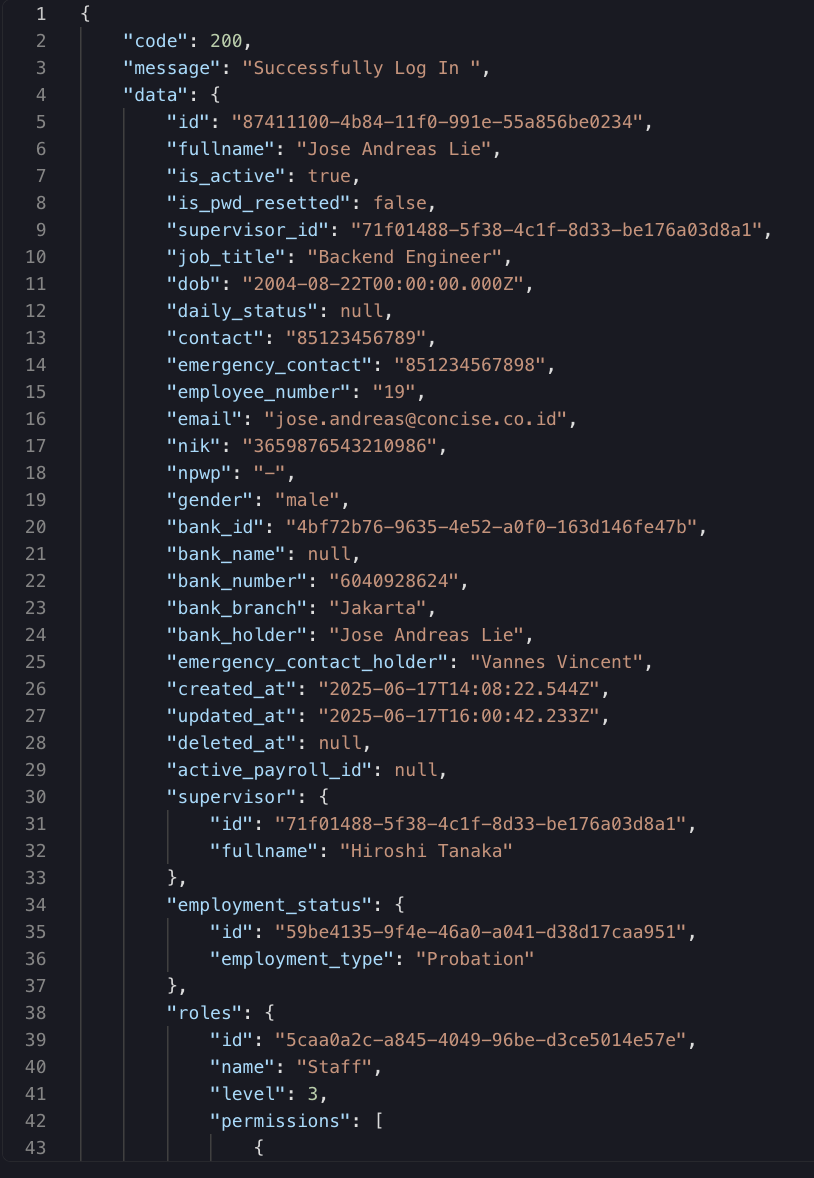
\includegraphics[width=0.8\textwidth]{assets/pics/fig_response_biometric_login.png}}
    \caption{Contoh struktur \textit{response} untuk \texttt{/auth/biometric/login}}
    \label{fig:response_biometric_login}
\end{figure}

Pada gambar \ref{fig:request_biometric_login}, terlihat struktur \textit{request} yang dikirimkan ke \textit{endpoint} \texttt{/auth/biometric/login}. Data yang dikirim hanya berupa nilai \textit{biometric} yang berisi string acak sepanjang 255 karakter yang telah dibuat dan disimpan di storage lokal CHRISM saat proses registrasi biometrik sebelumnya. Nilai ini berfungsi sebagai representasi dari data biometrik pengguna. Setelah \textit{request} berhasil diproses, sistem akan mengembalikan respons seperti pada gambar \ref{fig:response_biometric_login}, yang menunjukkan bahwa autentikasi pegawai menggunakan data biometrik berhasil dengan kode status 200 (\textit{OK}), pesan yang sesuai dan data lainnya.


% ---------------------------------------- %
\subsection{Implementasi \textit{Leave Permit}}
% -------------------- %
\subsubsection{API \textit{Endpoints}}
% -------------------- %
Berikut adalah daftar \textit{endpoint} yang telah ditambahkan untuk modul \textit{Leave Permit}:
\begin{center}
    \begin{longtable}{|c|p{0.37\textwidth}|c|p{0.33\textwidth}|}
    \caption{\textit{Leave Permit} API \textit{Endpoints}} 
    \label{tab:tbl_leave_permit} \\
    \hline
    \textbf{No.} & \textbf{Endpoint} & \textbf{Method} & \textbf{Deskripsi Singkat} \\
    \hline
    \endfirsthead

    \multicolumn{4}{c}%
    {{\tablename\ \thetable{} \textit{Leave Permit} API \textit{Endpoints} (lanjutan)}} \\
    \hline
    \textbf{No.} & \textbf{Endpoint} & \textbf{Method} & \textbf{Deskripsi Singkat} \\
    \hline
    \endhead

    \hline 
    \multicolumn{4}{|r|}{{Lanjut di halaman berikutnya}} \\
    \hline
    \endfoot

    \hline
    \endlastfoot

    1 & \texttt{/leave-permit} & GET & Menampilkan data leave permit pada user yang login. \\ \hline
    2 & \texttt{/leave-permit/{:id}} & GET & Mengambil data leave permit berdasarkan id. \\ \hline
    3 & \texttt{/leave-permit} & POST & Membuat data leave permit baru. \\ \hline
    4 & \texttt{/leave-permit/{:id}} & DELETE & Menghapus data leave permit berdasarkan id. \\ \hline
    5 & \texttt{/leave-permit/dashboard} & GET & Mengambil data leave permit yang telah diterima oleh atasan dan yang berjalan di minggu ini untuk dashboard page. \\ \hline
    6 & \texttt{/leave-permit/all} & GET & Mengambil data leave permit berdasarkan hirarki atasan. \\ \hline
    \end{longtable}
\end{center}

Pada Tabel \ref{tab:tbl_leave_permit}, ditampilkan sebagian \textit{endpoint} yang telah dimodifikasi dan ditambahkan untuk modul \textit{Leave Permit}. Tabel ini tidak mencakup seluruh \textit{endpoint} yang ada, melainkan hanya yang relevan dengan pengembangan selama masa kerja praktik. Setiap \textit{endpoint} dilengkapi dengan metode HTTP yang sesuai dengan tujuannya: \textit{GET} digunakan untuk mengambil data dari basis data, \textit{POST} digunakan untuk pembuatan data baru, dan \textit{DELETE} digunakan untuk menghapus data.


% -------------------- %
\subsubsection{Contoh \textit{Request} dan \textit{Response}}
% -------------------- %
\begin{figure}
    \centering
    \fbox{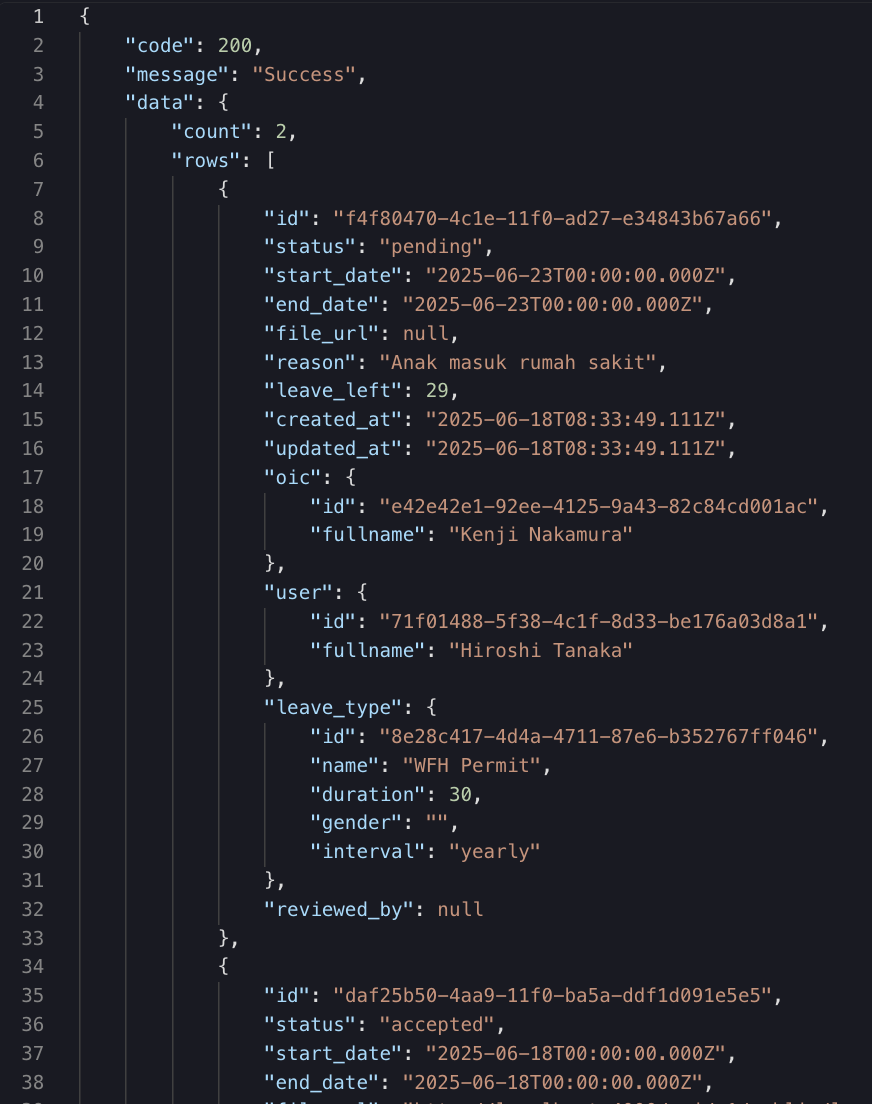
\includegraphics[width=0.8\textwidth]{assets/pics/fig_response_leave_permit_get.png}}
    \caption{Contoh struktur \textit{response} untuk GET \texttt{/leave-permit}}
    \label{fig:response_leave_permit}
\end{figure}
Pada gambar \ref{fig:response_leave_permit}, terlihat struktur \textit{response} yang dikembalikan oleh sistem ketika melakukan permintaan GET ke \textit{endpoint} \texttt{/leave-permit}. Respons ini berisi daftar permohonan cuti yang telah dibuat oleh pegawai yang sedang login, dengan informasi seperti id, jenis cuti, tanggal mulai dan berakhir, status permohonan dan lain-lain.


\begin{figure}
    \centering
    \fbox{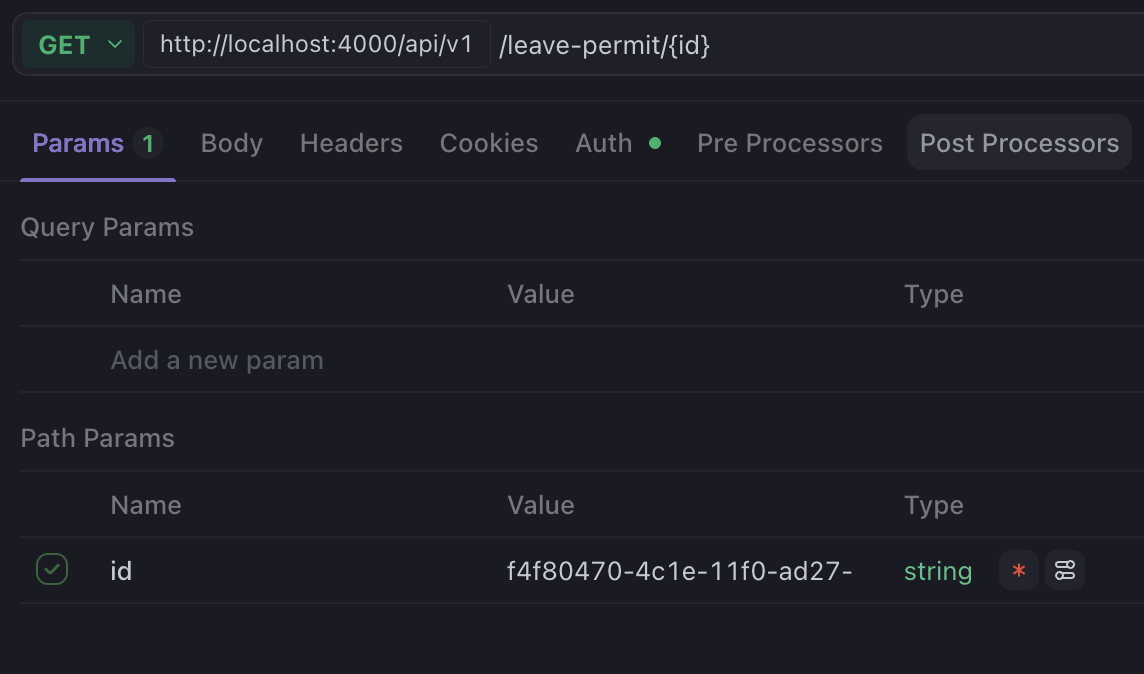
\includegraphics[width=0.8\textwidth]{assets/pics/fig_request_leave_permit_by_id_get.png}}
    \caption{Contoh struktur \textit{request} untuk GET \texttt{/leave-permit/{id}}}
    \label{fig:request_leave_permit_by_id_get}
\end{figure}

\begin{figure}
    \centering
    \fbox{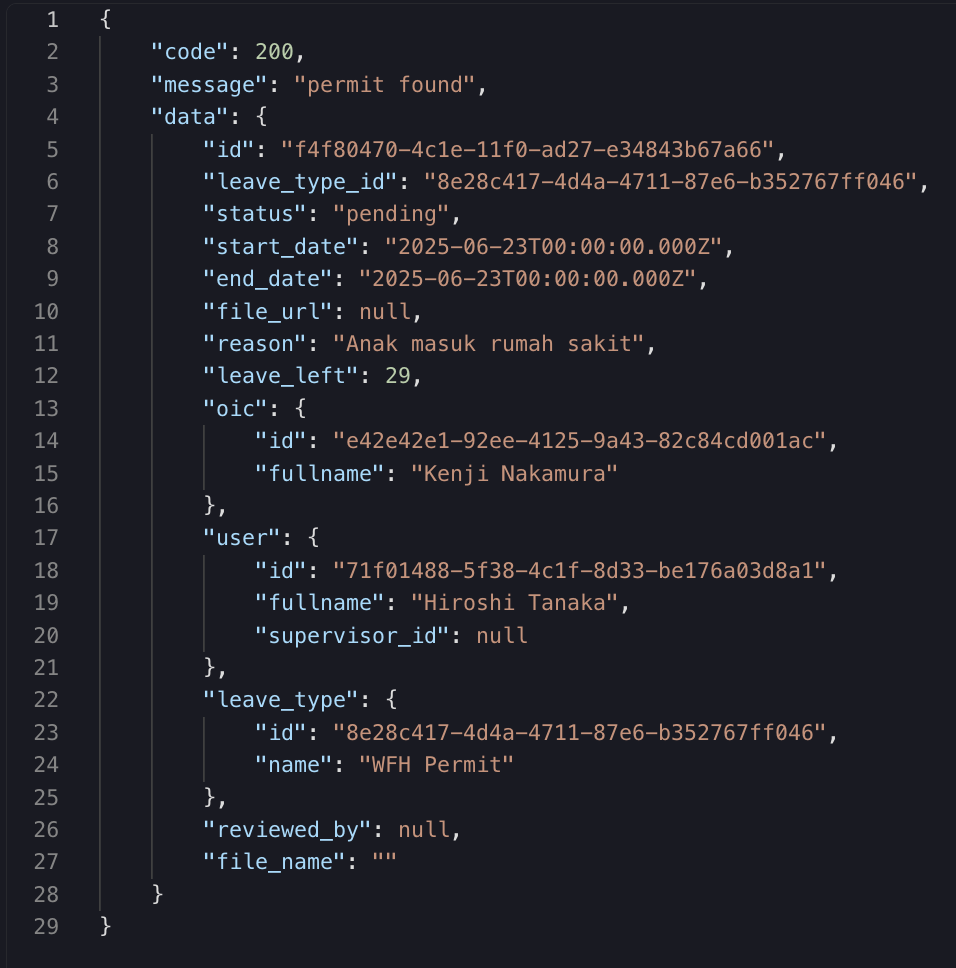
\includegraphics[width=0.8\textwidth]{assets/pics/fig_response_leave_permit_by_id_get.png}}
    \caption{Contoh struktur \textit{response} untuk GET \texttt{/leave-permit/{:id}}}
    \label{fig:response_leave_permit_by_id_get}
\end{figure}

Pada gambar \ref{fig:request_leave_permit_by_id_get}, terlihat struktur \textit{request} yang dikirimkan ke \textit{endpoint} \texttt{/leave-permit/{id}}. Data yang dikirim hanya berupa \textit{id} permohonan cuti yang ingin diambil datanya. Setelah \textit{request} berhasil diproses, sistem akan mengembalikan respons seperti pada gambar \ref{fig:response_leave_permit_by_id_get}, yang menunjukkan bahwa pengambilan data leave permit berdasarkan id berhasil dengan kode status 200 (\textit{OK}) dan pesan yang sesuai.


\begin{figure}
    \centering
    \fbox{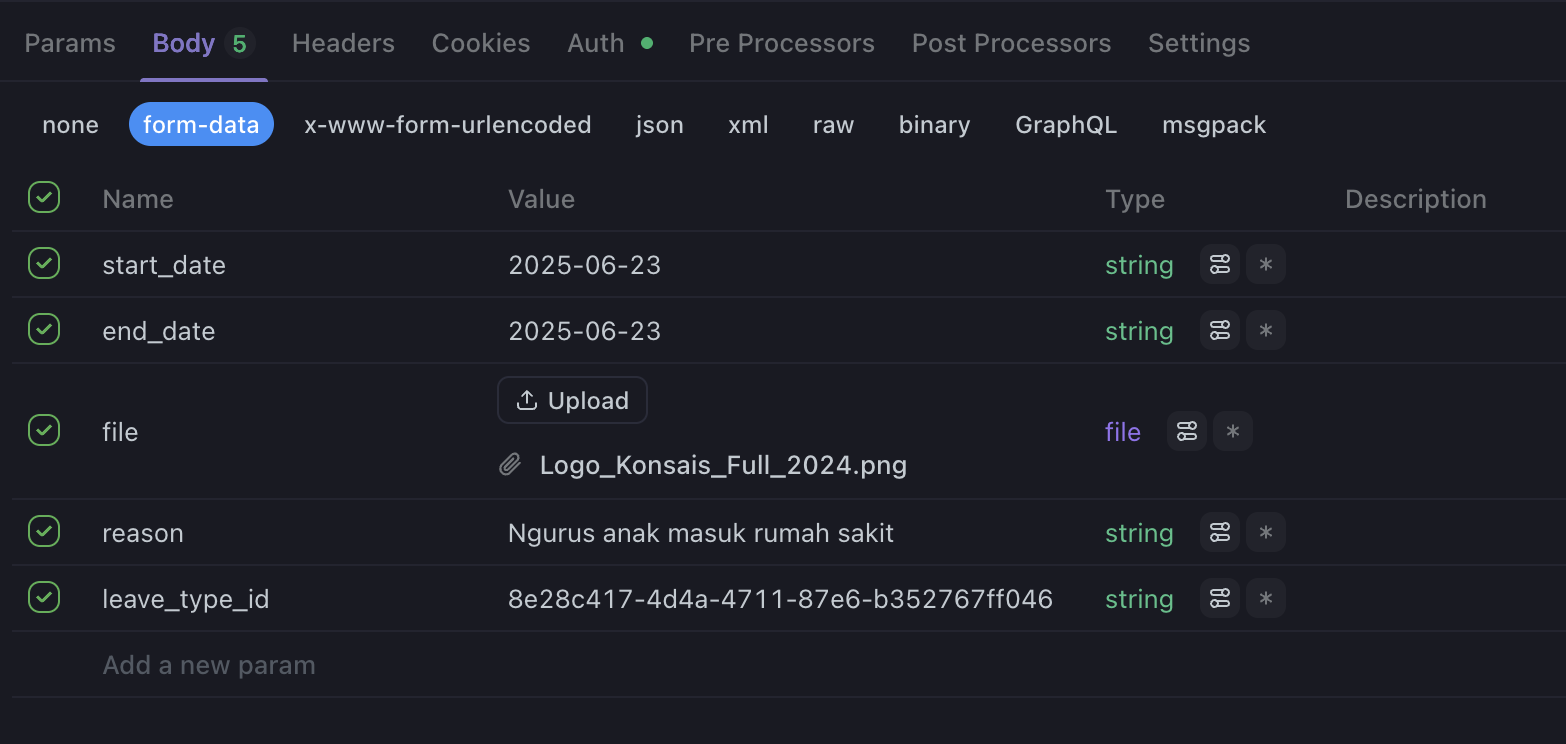
\includegraphics[width=0.8\textwidth]{assets/pics/fig_request_leave_permit_post.png}}
    \caption{Contoh struktur \textit{request} untuk POST \texttt{/leave-permit}}
    \label{fig:request_leave_permit}
\end{figure}
\begin{figure}
    \centering
    \fbox{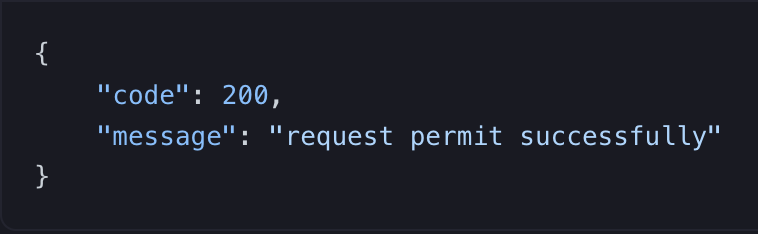
\includegraphics[width=0.8\textwidth]{assets/pics/fig_response_leave_permit_post.png}}
    \caption{Contoh struktur \textit{response} untuk POST \texttt{/leave-permit}}
    \label{fig:response_leave_permit}
\end{figure}
Pada gambar \ref{fig:request_leave_permit}, terlihat struktur \textit{request} yang dikirimkan ke \textit{endpoint} \texttt{/leave-permit}. Data yang dikirim berupa informasi terkait permohonan cuti, seperti jenis cuti, tanggal mulai dan berakhir, serta alasan permohonan. Setelah \textit{request} berhasil diproses, sistem akan mengembalikan respons seperti pada gambar \ref{fig:response_leave_permit}, yang menunjukkan bahwa pembuatan data leave permit berhasil dengan kode status 201 (\textit{Created}) dan pesan yang sesuai.

\begin{figure}
    \centering
    \fbox{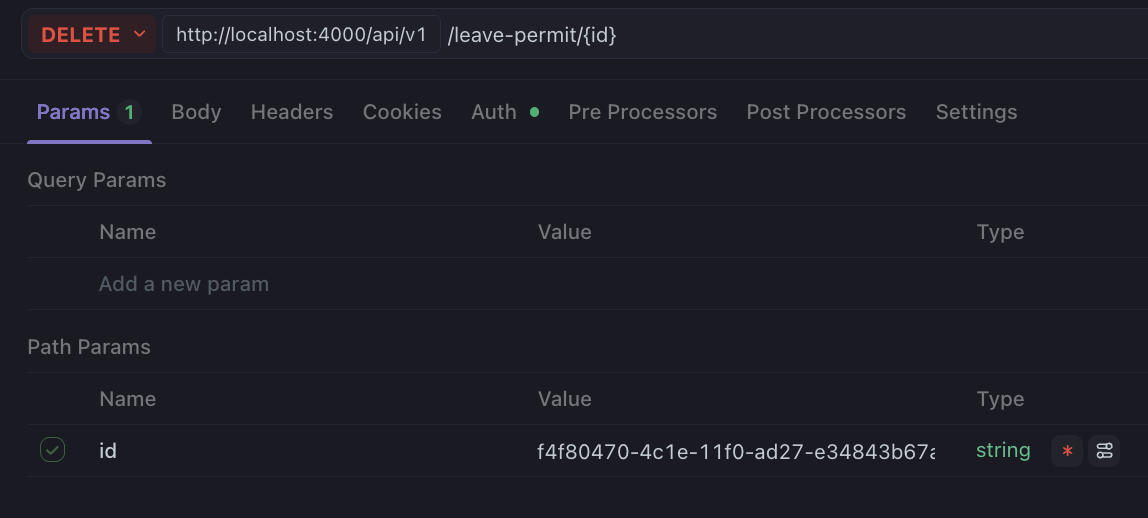
\includegraphics[width=0.8\textwidth]{assets/pics/fig_request_leave_permit_by_id_delete.png}}
    \caption{Contoh struktur \textit{request} untuk DELETE \texttt{/leave-permit}}
    \label{fig:request_leave_permit}
\end{figure}

\begin{figure}
    \centering
    \fbox{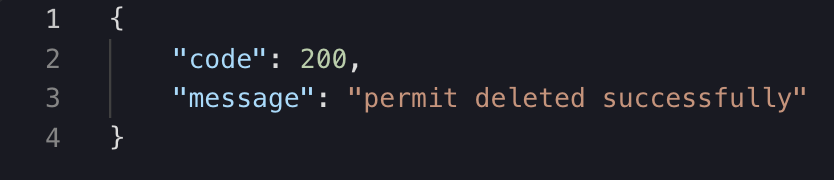
\includegraphics[width=0.8\textwidth]{assets/pics/fig_response_leave_permit_by_id_delete.png}}
    \caption{Contoh struktur \textit{response} untuk DELETE \texttt{/leave-permit/{:id}}}
    \label{fig:response_leave_permit_by_id_get}
\end{figure}

Pada gambar \ref{fig:request_leave_permit_by_id_delete}, terlihat struktur \textit{request} yang dikirimkan ke \textit{endpoint} \texttt{/leave-permit/{id}}. Data yang dikirim hanya berupa \textit{id} permohonan cuti yang ingin dihapus. Setelah \textit{request} berhasil diproses, sistem akan mengembalikan respons seperti pada gambar \ref{fig:response_leave_permit_by_id_get}, yang menunjukkan bahwa penghapusan data leave permit berdasarkan id berhasil dengan kode status 200 (\textit{OK}) dan pesan yang sesuai.


\begin{figure}
    \centering
    \fbox{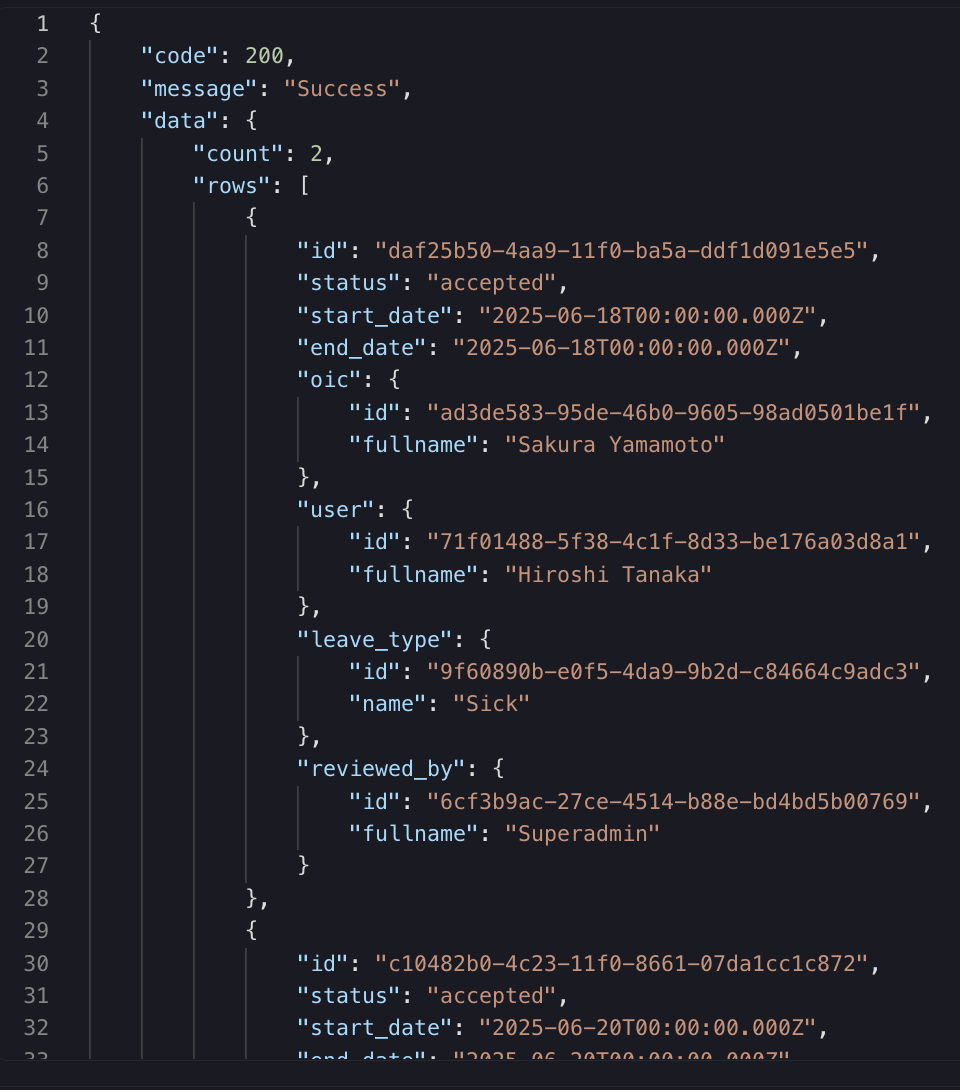
\includegraphics[width=0.8\textwidth]{assets/pics/fig_response_leave_permit_dashboard_get.png}}
    \caption{Contoh struktur \textit{response} untuk GET \texttt{/leave-permit/dashboard}}
    \label{fig:response_leave_permit_dashboard_get}
\end{figure}
Pada gambar \ref{fig:response_leave_permit_dashboard_get}, terlihat struktur \textit{response} yang dikembalikan oleh sistem ketika melakukan permintaan GET ke \textit{endpoint} \texttt{/leave-permit/dashboard}. Respons ini berisi data leave permit yang telah diterima oleh atasan dan yang sedang berjalan di minggu ini, dengan informasi seperti id, jenis cuti, tanggal mulai dan berakhir, status permohonan, pegawai yang mengajukan cuti, pegawai yang menerima cuti, dan \textit{officer in charge} yang dipilih. Data ini digunakan untuk menampilkan informasi terkait permohonan cuti pada halaman dashboard.


\begin{figure}
    \centering
    \fbox{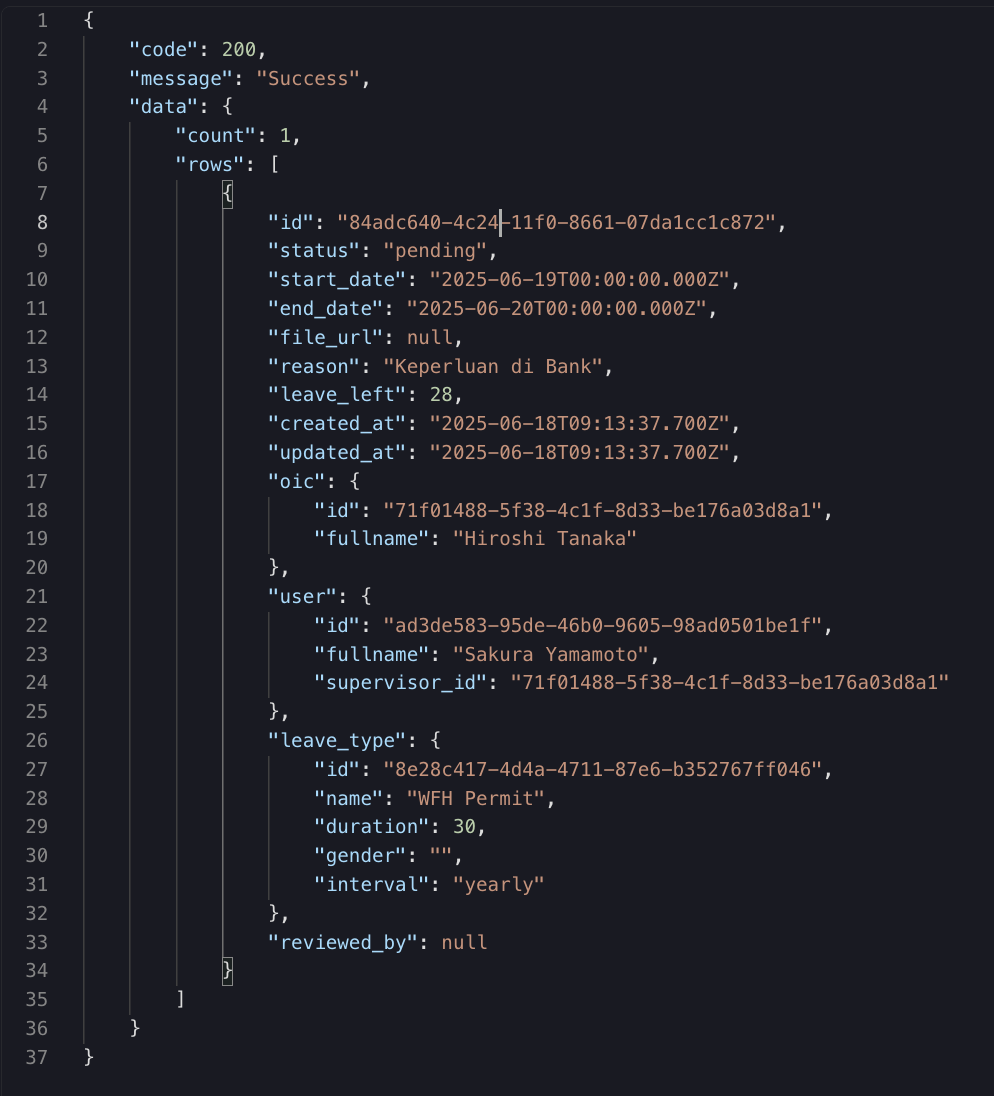
\includegraphics[width=0.8\textwidth]{assets/pics/fig_response_leave_permit_all_get.png}}
    \caption{Contoh struktur \textit{response} untuk GET \texttt{/leave-permit/all}}
    \label{fig:response_leave_permit_all_get}
\end{figure}
Pada gambar \ref{fig:response_leave_permit_all_get}, terlihat struktur \textit{response} yang dikembalikan oleh sistem ketika melakukan permintaan GET ke \textit{endpoint} \texttt{/leave-permit/all}. Respons ini berisi data leave permit berdasarkan hirarki atasan, dengan informasi seperti id, jenis cuti, tanggal mulai dan berakhir, status permohonan, pegawai yang mengajukan cuti, pegawai yang menerima cuti, dan \textit{officer in charge} yang dipilih. Data ini digunakan untuk menampilkan informasi terkait permohonan cuti pada halaman yang dapat diakses oleh atasan.
% ---------------------------------------- %

% ---------------------------------------- %
\subsection{Implementasi \textit{Payroll}}
\subsubsection{API \textit{Endpoints}}
Berikut adalah daftar \textit{endpoint} yang telah ditambahkan untuk modul \textit{Payroll}:
\begin{center}
    \begin{longtable}{|c|p{0.4\textwidth}|c|p{0.3\textwidth}|}
    \caption{\textit{Payroll} API \textit{Endpoints}} 
    \label{tab:tbl_payroll_endpoints} \\
    \hline
    \textbf{No.} & \textbf{Endpoint} & \textbf{Method} & \textbf{Deskripsi Singkat} \\
    \hline
    \endfirsthead

    \multicolumn{4}{c}%
    {{\tablename\ \thetable{} \textit{Payroll} API \textit{Endpoints} (lanjutan)}} \\
    \hline
    \textbf{No.} & \textbf{Endpoint} & \textbf{Method} & \textbf{Deskripsi Singkat} \\
    \hline
    \endhead

    \hline 
    \multicolumn{4}{|r|}{{Lanjut di halaman berikutnya}} \\
    \hline
    \endfoot

    \hline  
    \endlastfoot

    1 & \texttt{/payroll-configuration/all} & GET & Mengambil daftar data konfigurasi penggajian yang telah dibuat. \\ \hline
    2 & \texttt{/payroll-configuration/{:id}} & GET & Mengambil data konfigurasi penggajian berdasarkan id. \\ \hline
    3 & \texttt{/payroll-configuration} & POST & Membuat data konfigurasi penggajian baru. \\ \hline
    4 & \texttt{/payroll-configuration/{:id}} & DELETE & Menghapus data konfigurasi penggajian berdasarkan id. \\ \hline
    5 & \texttt{/payroll-configuration/{:id}} & PATCH & Mengubah data konfigurasi penggajian berdasarkan id. \\ \hline

    6 & \texttt{/users/{:user\_id}/ payroll-configuration} & GET & Mengambil daftar data konfigurasi penggajian berdasarkan id pegawai. \\ \hline
    7 & \texttt{/users/{:user\_id}/salary} & GET & Mengambil data gaji pegawai berdasarkan id pegawai. \\ \hline
    8 & \texttt{/user-allowance/ {:user\_id}/ {:payroll\_configuration\_id}} & GET & Mengambil data tunjangan berdasarkan id pegawai dan id konfigurasi penggajian. \\ \hline
    9 & \texttt{/users/{:user\_id}/ with-details} & PATCH & Menyimpan data pegawai, gaji, dan semua tunjangan yang sudah dikirimkan. \\ \hline
    10 & \texttt{/salary-slip/all?date=YYYY-MM} & GET & Mengambil daftar slip gaji pegawai yang telah dibuat. \\ \hline
    11 & \texttt{/salary-slip/{:id}} & GET & Mengambil data slip gaji pegawai berdasarkan id. \\ \hline
    12 & \texttt{/salary-slip?date=YYYY-MM} & GET & Mengambil data slip gaji pengguna yang sedang aktif pada bulan tertentu. \\ \hline
    \end{longtable}
\end{center}

Pada Tabel \ref{tab:tbl_payroll_endpoints}, ditampilkan daftar \textit{endpoint} yang telah ditambahkan untuk modul \textit{Payroll}. Setiap \textit{endpoint} dilengkapi dengan metode HTTP yang sesuai dengan tujuannya: \textit{GET} digunakan untuk mengambil data dari basis data, \textit{POST} digunakan untuk pembuatan data baru, \textit{DELETE} digunakan untuk menghapus data, dan \textit{PATCH} digunakan untuk memperbarui data yang ada.

\subsubsection{Contoh \textit{Request} dan \textit{Response}}
\begin{figure}
    \centering
    \fbox{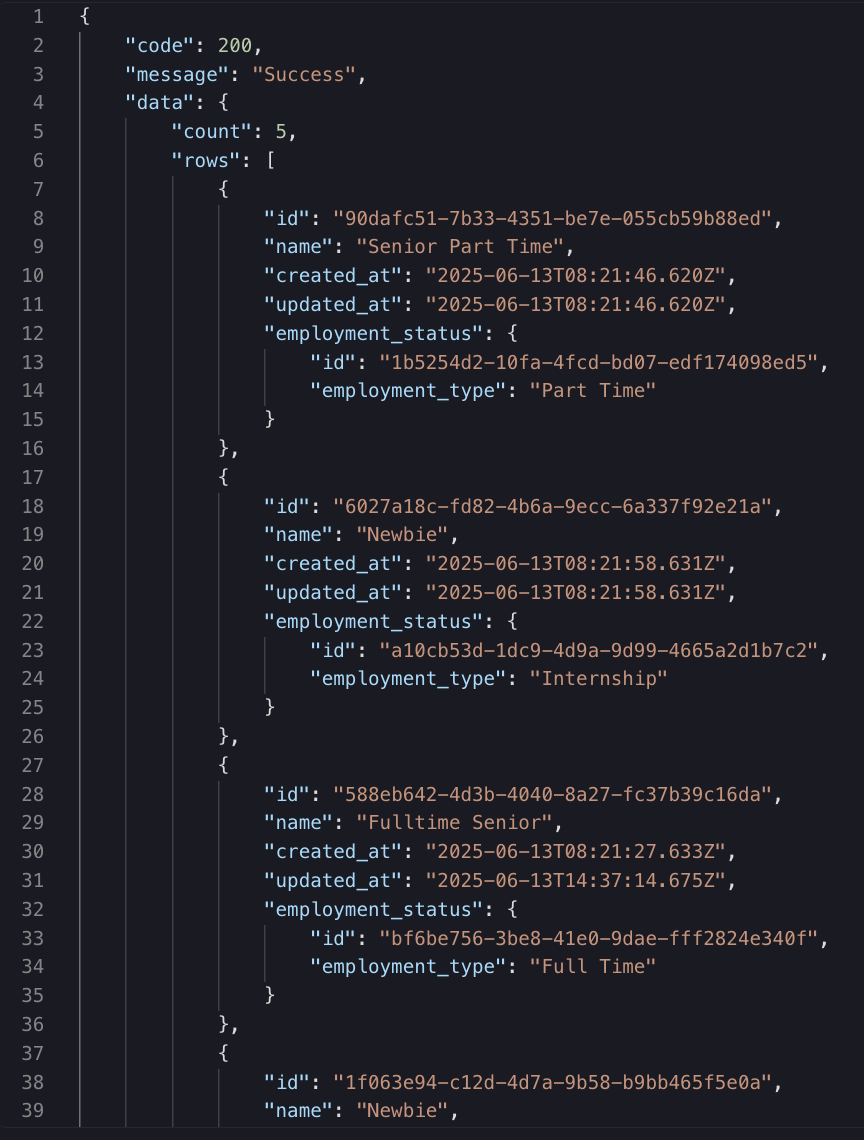
\includegraphics[width=0.8\textwidth]{assets/pics/fig_response_payroll_configuration_all_get.png}}
    \caption{Contoh struktur \textit{request} untuk GET \texttt{/payroll-configuration/all}}
    \label{fig:response_payroll_configuration_all_get}
\end{figure}
Pada gambar \ref{fig:response_payroll_configuration_all_get}, terlihat struktur \textit{response} yang dikembalikan oleh sistem ketika melakukan permintaan GET ke \textit{endpoint} \texttt{/payroll-configuration/all}. Respons ini berisi daftar konfigurasi penggajian yang telah dibuat, dengan informasi seperti id, nama konfigurasi, dan status kepegawaian.

\begin{figure}
    \centering
    \fbox{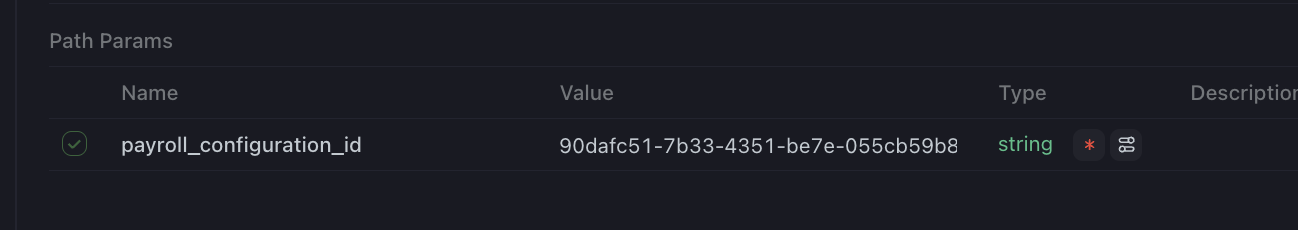
\includegraphics[width=0.8\textwidth]{assets/pics/fig_request_payroll_configuration_by_id_get.png}}
    \caption{Contoh struktur \textit{request} untuk GET \texttt{/payroll-configuration/{:id}}}
    \label{fig:request_payroll_configuration_by_id_get}
\end{figure}
\begin{figure}
    \centering
    \fbox{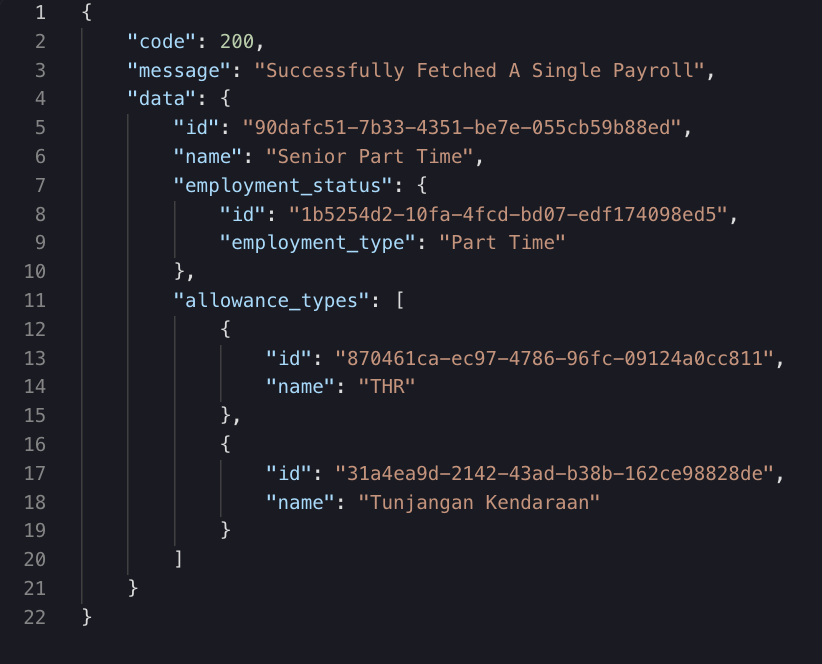
\includegraphics[width=0.8\textwidth]{assets/pics/fig_response_payroll_configuration_by_id_get.png}}
    \caption{Contoh struktur \textit{response} untuk GET \texttt{/payroll-configuration/{:id}}}
    \label{fig:response_payroll_configuration_by_id_get}
\end{figure}
Pada gambar \ref{fig:request_payroll_configuration_by_id_get}, terlihat struktur \textit{request} yang dikirimkan ke \textit{endpoint} \texttt{/payroll-configuration/{id}}. Data yang dikirim hanya berupa \textit{id} konfigurasi penggajian yang ingin diambil datanya. Setelah \textit{request} berhasil diproses, sistem akan mengembalikan respons seperti pada gambar \ref{fig:response_payroll_configuration_by_id_get}, yang menunjukkan bahwa pengambilan data konfigurasi penggajian berdasarkan id berhasil dengan kode status 200 (\textit{OK}) dan pesan yang sesuai.


\begin{figure}
    \centering
    \fbox{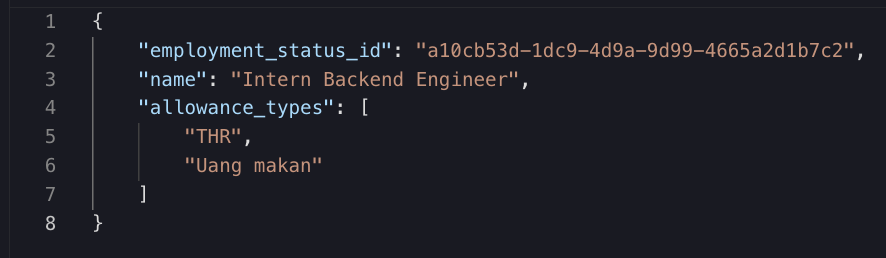
\includegraphics[width=0.8\textwidth]{assets/pics/fig_request_payroll_configuration_post.png}}
    \caption{Contoh struktur \textit{request} untuk POST \texttt{/payroll-configuration}}
    \label{fig:request_payroll_configuration_post}
\end{figure}
\begin{figure}
    \centering
    \fbox{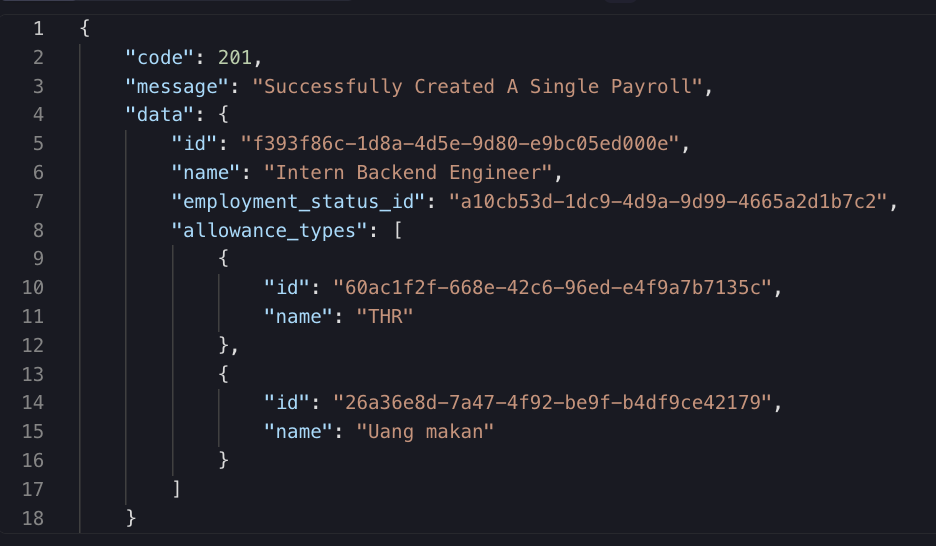
\includegraphics[width=0.8\textwidth]{assets/pics/fig_response_payroll_configuration_post.png}}
    \caption{Contoh struktur \textit{response} untuk POST \texttt{/payroll-configuration}}
    \label{fig:response_payroll_configuration_post}
\end{figure}
Pada gambar \ref{fig:request_payroll_configuration_post}, terlihat struktur \textit{request} yang dikirimkan ke \textit{endpoint} \texttt{/payroll-configuration}. Data yang dikirim berupa informasi terkait konfigurasi penggajian, seperti nama konfigurasi, status kepegawaian, dan tunjangan-tunjangan. Setelah \textit{request} berhasil diproses, sistem akan mengembalikan respons seperti pada gambar \ref{fig:response_payroll_configuration_post}, yang menunjukkan bahwa pembuatan data konfigurasi penggajian berhasil dengan kode status 201 (\textit{Created}) dan pesan yang sesuai.

\begin{figure}
    \centering
    \fbox{\includegraphics[width=0.8\textwidth]{assets/pics/fig_request_payroll_configuration_by_id_delete.png}}
    \caption{Contoh struktur \textit{request} untuk DELETE \texttt{/payroll-configuration/{:id}}}
    \label{fig:request_payroll_configuration_by_id_delete}
\end{figure}
\begin{figure}
    \centering
    \fbox{\includegraphics[width=0.8\textwidth]{assets/pics/fig_response_payroll_configuration_by_id_delete.png}}
    \caption{Contoh struktur \textit{response} untuk DELETE \texttt{/payroll-configuration/{:id}}}
    \label{fig:response_payroll_configuration_by_id_delete}
\end{figure}

Pada gambar \ref{fig:request_payroll_configuration_by_id_delete}, terlihat struktur \textit{request} yang dikirimkan ke \textit{endpoint} \texttt{/payroll-configuration/{id}}. Data yang dikirim hanya berupa \textit{id} konfigurasi penggajian yang ingin dihapus. Setelah \textit{request} berhasil diproses, sistem akan mengembalikan respons seperti pada gambar \ref{fig:response_payroll_configuration_by_id_delete}, yang menunjukkan bahwa penghapusan data konfigurasi penggajian berdasarkan id berhasil dengan kode status 200 (\textit{OK}) dan pesan yang sesuai.

\begin{figure}
    \centering
    \fbox{\includegraphics[width=0.8\textwidth]{assets/pics/fig_params_payroll_configuration_by_id_patch.png}}
    \caption{Contoh struktur \textit{params} untuk PATCH \texttt{/payroll-configuration/{:id}}}
    \label{fig:request_payroll_configuration_by_id_patch}
\end{figure}

\begin{figure}
    \centering
    \fbox{\includegraphics[width=0.8\textwidth]{assets/pics/fig_request_payroll_configuration_by_id_patch.png}}
    \caption{Contoh struktur \textit{request} untuk PATCH \texttt{/payroll-configuration/{:id}}}
    \label{fig:request_payroll_configuration_by_id_patch}
\end{figure}

\begin{figure}
    \centering
    \fbox{\includegraphics[width=0.8\textwidth]{assets/pics/fig_response_payroll_configuration_by_id_patch.png}}
    \caption{Contoh struktur \textit{response} untuk PATCH \texttt{/payroll-configuration/{:id}}}
    \label{fig:response_payroll_configuration_by_id_patch}
\end{figure}

Pada gambar \ref{fig:params_payroll_configuration_by_id_patch}, terlihat parameter yang dikirimkan ke path \textit{endpoint} \texttt{/payroll-configuration/{:id}} yang berisi ID konfigurasi penggajian yang ingin dimodifikasi. Sementara pada gambar \ref{fig:request_payroll_configuration_by_id_patch}, terlihat struktur \textit{request body} yang berisi field-field yang ingin direvisi, seperti nama konfigurasi, status kepegawaian, dan tunjangan-tunjangan. Setelah \textit{request} berhasil diproses, sistem akan mengembalikan respons seperti pada gambar \ref{fig:response_payroll_configuration_by_id_patch}, yang menunjukkan bahwa pembaruan data konfigurasi penggajian berdasarkan id berhasil dengan kode status 200 (\textit{OK}) dan pesan yang sesuai.

\begin{figure}
    \centering
    \fbox{\includegraphics[width=0.8\textwidth]{assets/pics/fig_request_users_payroll_configuration_by_user_id_get.png}}
    \caption{Contoh struktur \textit{request} untuk GET \texttt{/users/{:user\_id}/ payroll-configuration}}
    \label{fig:response_payroll_configuration_by_user_id_get}
\end{figure}
\begin{figure}
    \centering
    \fbox{\includegraphics[width=0.8\textwidth]{assets/pics/fig_response_users_payroll_configuration_by_user_id_get.png}}
    \caption{Contoh struktur \textit{response} untuk GET \texttt{/users/{:user\_id}/ payroll-configuration}}
    \label{fig:request_payroll_configuration_by_user_id_get}
\end{figure}
Pada gambar \ref{fig:request_payroll_configuration_by_user_id_get}, terlihat struktur \textit{request} yang dikirimkan ke \textit{endpoint} \texttt{/users/{:user\_id}/payroll-configuration}, yang berisi parameter id pegawai yang ingin diambil data konfigurasi penggajiannya. Setelah \textit{request} berhasil diproses, sistem akan mengembalikan respons seperti pada gambar \ref{fig:response_payroll_configuration_by_user_id_get}, yang menunjukkan daftar konfigurasi penggajian yang tersedia berdasarkan status kepegawaian pegawai tersebut, dengan kode status 200 (\textit{OK}) dan pesan yang sesuai.


\begin{figure}
    \centering
    \fbox{\includegraphics[width=0.8\textwidth]{assets/pics/fig_request_users_salary_by_user_id_get.png}}
    \caption{Contoh struktur \textit{request} untuk GET \texttt{/users/{:user\_id}/salary}}
    \label{fig:request_users_salary_by_user_id_get}
\end{figure}
\begin{figure}
    \centering
    \fbox{\includegraphics[width=0.8\textwidth]{assets/pics/fig_response_users_salary_by_user_id_get.png}}
    \caption{Contoh struktur \textit{response} untuk GET \texttt{/users/{:user\_id}/salary}}
    \label{fig:response_users_salary_by_user_id_get}
\end{figure}

Pada gambar \ref{fig:request_users_salary_by_user_id_get}, terlihat struktur \textit{request} yang dikirimkan ke \textit{endpoint} \texttt{/users/{:user\_id}/salary}, yang berisi parameter id pegawai yang ingin diambil data gajinya. Setelah \textit{request} berhasil diproses, sistem akan mengembalikan respons seperti pada gambar \ref{fig:response_users_salary_by_user_id_get}, yang menunjukkan data gaji pegawai berdasarkan id pegawai tersebut, dengan kode status 200 (\textit{OK}) dan pesan yang sesuai.

\begin{figure}
    \centering
    \fbox{\includegraphics[width=0.8\textwidth]{assets/pics/fig_request_user_allowance_by_user_id_and_payroll_configuration_id_get.png}}
    \caption{Contoh struktur \textit{request} untuk GET \texttt{/user-allowance/{:user\_id}/ {:payroll\_configuration\_id}}}
    \label{fig:request_user_allowance_by_user_id_and_payroll_configuration_id_get}
\end{figure}
\begin{figure}
    \centering
    \fbox{\includegraphics[width=0.8\textwidth]{assets/pics/fig_response_user_allowance_by_user_id_and_payroll_configuration_id_get.png}}
    \caption{Contoh struktur \textit{response} untuk GET \texttt{/user-allowance/{:user\_id}/ {:payroll\_configuration\_id}}}
    \label{fig:response_user_allowance_by_user_id_and_payroll_configuration_id_get}
\end{figure}
Pada gambar \ref{fig:request_user_allowance_by_user_id_and_payroll_configuration_id_get}, terlihat struktur \textit{request} yang dikirimkan ke \textit{endpoint} \texttt{/user-allowance/{:user\_id}/ {:payroll\_configuration\_id}}, yang berisi parameter id pegawai dan id konfigurasi penggajian yang ingin diambil data tunjangannya. Setelah \textit{request} berhasil diproses, sistem akan mengembalikan respons seperti pada gambar \ref{fig:response_user_allowance_by_user_id_and_payroll_configuration_id_get}, yang menunjukkan data tunjangan pegawai berdasarkan id pegawai dan id konfigurasi penggajian tersebut, dengan kode status 200 (\textit{OK}) dan pesan yang sesuai.

\begin{figure}
    \centering
    \fbox{\includegraphics[width=0.8\textwidth]{assets/pics/fig_params_users_with_details_patch.png}}
    \caption{Contoh struktur \textit{params} untuk PATCH \texttt{/users/{:user\_id}/ with-details}}
    \label{fig:params_users_with_details_patch}
\end{figure}
\begin{figure}
    \centering
    \fbox{\includegraphics[width=0.8\textwidth]{assets/pics/fig_request_users_with_details_patch.png}}
    \caption{Contoh struktur \textit{request} untuk PATCH \texttt{/users/{:user\_id}/ with-details}}
    \label{fig:request_users_with_details_patch}
\end{figure}
\begin{figure}
    \centering
    \fbox{\includegraphics[width=0.8\textwidth]{assets/pics/fig_response_users_with_details_patch.png}}
    \caption{Contoh struktur \textit{response} untuk PATCH \texttt{/users/{:user\_id}/ with-details}}
    \label{fig:response_users_with_details_patch}
\end{figure}

Pada gambar \ref{fig:params_users_with_details_patch}, terlihat parameter yang dikirimkan ke path \textit{endpoint} \texttt{/users/{:user\_id}/ with-details} yang berisi ID pegawai yang ingin dimodifikasi. Sementara pada gambar \ref{fig:request_users_with_details_patch}, terlihat struktur \textit{request body} yang berisi field-field yang ingin direvisi, seperti data pegawai, gaji, dan tunjangan-tunjangan. Setelah \textit{request} berhasil diproses, sistem akan mengembalikan respons seperti pada gambar \ref{fig:response_users_with_details_patch}, yang menunjukkan bahwa pembaruan data pegawai, gaji, dan tunjangan berdasarkan id pegawai berhasil dengan kode status 200 (\textit{OK}) dan pesan yang sesuai.


\begin{figure}
    \centering
    \fbox{\includegraphics[width=0.8\textwidth]{assets/pics/fig_request_salary_slip_all_get.png}}
    \caption{Contoh struktur \textit{request} untuk GET \texttt{/salary-slip/all}}
    \label{fig:request_salary_slip_all_get}
\end{figure}

\begin{figure}
    \centering
    \fbox{\includegraphics[width=0.8\textwidth]{assets/pics/fig_response_salary_slip_all_get.png}}
    \caption{Contoh struktur \textit{response} untuk GET \texttt{/salary-slip/all}}
    \label{fig:response_salary_slip_all_get}
\end{figure}

Pada gambar \ref{fig:request_salary_slip_all_get}, terlihat struktur \textit{request} yang dikirimkan ke \textit{endpoint} \texttt{/salary-slip/all}, yang berisi query parameter \texttt{date=YYYY-MM} untuk menyaring slip gaji pada bulan dan tahun tertentu. Setelah \textit{request} berhasil diproses, sistem akan mengembalikan respons seperti pada gambar \ref{fig:response_salary_slip_all_get}, yang menunjukkan daftar slip gaji pegawai yang telah dibuat untuk periode yang diminta, dengan kode status 200 (\textit{OK}) dan pesan yang sesuai.

\begin{figure}
    \centering
    \fbox{\includegraphics[width=0.8\textwidth]{assets/pics/fig_request_salary_slip_by_user_id_get.png}}
    \caption{Contoh struktur \textit{request} untuk GET \texttt{/salary-slip/{:user\_id}}}
    \label{fig:request_salary_slip_by_id_get}
\end{figure}
\begin{figure}
    \centering
    \fbox{\includegraphics[width=0.8\textwidth]{assets/pics/fig_response_salary_slip_by_user_id_get.png}}
    \caption{Contoh struktur \textit{response} untuk GET \texttt{/salary-slip/{:user\_id}}}
    \label{fig:response_salary_slip_by_id_get}
\end{figure}

Pada gambar \ref{fig:request_salary_slip_by_id_get}, terlihat struktur \textit{request} yang dikirimkan ke \textit{endpoint} \texttt{/salary-slip/{:id}}, yang berisi parameter id pegawai yang ingin diambil datanya. Selain itu, terdapat query parameter \texttt{date=YYYY-MM} yang digunakan untuk menyaring slip gaji pada bulan dan tahun tertentu. Setelah \textit{request} berhasil diproses, sistem akan mengembalikan respons seperti pada gambar \ref{fig:response_salary_slip_by_id_get}, yang menunjukkan data slip gaji pegawai berdasarkan id pegawai tersebut pada periode waktu yang diminta, dengan kode status 200 (\textit{OK}) dan pesan yang sesuai.


\begin{figure}
    \centering
    \fbox{\includegraphics[width=0.8\textwidth]{assets/pics/fig_request_salary_slip_get.png}}
    \caption{Contoh struktur \textit{request} untuk GET \texttt{/salary-slip}}
    \label{fig:request_salary_slip_get}
\end{figure}
\begin{figure}
    \centering
    \fbox{\includegraphics[width=0.8\textwidth]{assets/pics/fig_response_salary_slip_get.png}}
    \caption{Contoh struktur \textit{response} untuk GET \texttt{/salary-slip?date=YYYY-MM}}
    \label{fig:response_salary_slip_get}
\end{figure}

Pada gambar \ref{fig:request_salary_slip_get}, terlihat struktur \textit{request} yang dikirimkan ke \textit{endpoint} \texttt{/salary-slip}, yang berisi query parameter \texttt{date=YYYY-MM} untuk menyaring slip gaji pada bulan dan tahun tertentu. Setelah \textit{request} berhasil diproses, sistem akan mengembalikan respons seperti pada gambar \ref{fig:response_salary_slip_get}, yang menunjukkan data slip gaji pengguna yang sedang aktif pada periode waktu yang diminta, dengan kode status 200 (\textit{OK}) dan pesan yang sesuai.

% ---------------------------------------- %
\section{Kendala dan Solusi yang Ditemukan}
% -------------------- %

\subsection{Kendala}
Selama pelaksanaan kerja praktik, ditemukan beberapa kendala teknis dan struktural dalam proses pengembangan sistem, yaitu sebagai berikut:
\begin{enumerate}
\item Beberapa bagian kode tidak mengikuti prinsip \textit{best practice} dalam pengembangan backend, sehingga menyulitkan proses pengembangan lanjutan dan pemeliharaan sistem.
\item Terdapat penggunaan nilai yang masih ditulis secara \textit{hardcoded}, seperti \textit{job title}, yang seharusnya dikelola melalui relasi ke dalam basis data agar lebih fleksibel dan dapat disesuaikan.
\item Modul Payroll memiliki kompleksitas tinggi, khususnya dalam pengambilan data historis pengguna, yang menjadi tantangan dalam perhitungan gaji berdasarkan riwayat data.
\item Proses \textit{migration} dan \textit{seeding} data belum optimal dan membutuhkan waktu lama karena struktur data yang belum efisien.
\end{enumerate}

\subsection{Solusi}
Berikut adalah langkah-langkah solusi yang dilakukan untuk mengatasi kendala-kendala tersebut:
\begin{enumerate}
    \item Melakukan proses \textit{code review} secara berkala bersama tim \textit{backend} untuk memastikan bahwa setiap kode yang ditulis mengikuti standar \textit{best practice} dan dapat dikembangkan dengan mudah di masa depan.
    \item Melakukan \textit{refactoring} pada bagian kode yang masih menggunakan pendekatan \textit{hardcoded}, seperti pengelolaan \textit{job title}, dengan menggantinya menjadi referensi ke tabel \textit{job\_titles}.
    \item Menambahkan tabel transaksi (\textit{transaction table}) pada modul Payroll untuk menyimpan data historis penggajian secara terpisah, sehingga proses perhitungan gaji dapat dilakukan secara lebih akurat dan efisien.
    \item Mengoptimalkan proses \textit{migration} dan \textit{seeding} dengan menyusun ulang struktur data serta membuat script yang lebih modular untuk mempercepat inisialisasi sistem.
\end{enumerate}



% -------------------- %
% -------------------- %
% -------------------- %
% -------------------- %
% -------------------- %
% -------------------- %
% -------------------- %
% -------------------- %
% -------------------- %
% -------------------- %
% ini cmd + enter
% \clearpage
% .
% \clearpage
% .
% \clearpage
% -------------------- %
% -------------------- %
% -------------------- %
% -------------------- %
% -------------------- %
% -------------------- %
% -------------------- %
% -------------------- %
% -------------------- %
% -------------------- %

% \section{Membuat Tabel}
% %-----------------------------------------------------------------------------%
% Seperti pada gambar, tabel juga dapat diberi label dan caption. 
% Caption pada tabel terletak pada bagian atas tabel. 
% Contoh tabel sederhana dapat dilihat pada \tab~\ref{tab:tab1}.

% \begin{table}
% 	\centering
% 	\caption{Contoh Tabel}
% 	\label{tab:tab1}
% 	\begin{tabular}{l | c r}
% 		\hline
% 		& kol 1 & kol 2 \\ 
% 		\hline
% 		baris 1 & 1 & 2 \\
% 		baris 2 & 3 & 4 \\
% 		baris 3 & 5 & 6 \\
% 		jumlah  & 9 & 12 \\
% 		\hline
% 	\end{tabular}
% \end{table}

% Ada jenis tabel lain yang dapat dibuat dengan \latex~berikut 
% beberapa di antaranya. 
% Contoh-contoh ini bersumber dari 
% \url{http://en.wikibooks.org/wiki/LaTeX/Tables}

% \begin{table}
% 	\centering
% 	\caption{An example of rows spanning multiple columns}
% 	\label{row.spanning}
% 	\begin{tabular}{l l *{6}{c}}
%   		\hline % create horizontal line
%   		No & Name & \multicolumn{3}{c}{Week 1} & \multicolumn{3}{c}{Week 2} \\
%   		\cline{3-8} % create line from 3rd column till 8th column
%   		& & A & B & C & A & B & C\\
%   		\hline
%   		1 & Lala & 1 & 2 & 3 & 4 & 5 & 6\\
%   		2 & Lili & 1 & 2 & 3 & 4 & 5 & 6\\
%   		3 & Lulu & 1 & 2 & 3 & 4 & 5 & 6\\
%   		\hline
% 	\end{tabular}
% \end{table}

% \lipsum[43-44]

% \begin{table}
% 	\centering
% 	\caption{Penulisan judul tabel dan judul gambar adalah rata kiri kanan serta tidak dicetak tebal dan mengikuti cara penulisan kalimat (sentence case).}
% 	\label{column.spanning}
% 	\begin{tabular}{l c l}
% 		\hline
% 		Percobaan & Iterasi & Waktu \\
% 		\hline
% 		Pertama & 1 & 0.1 sec \\ \hline
% 		\multirow{2}{*}{Kedua} & 1 & 0.1 sec \\
%  		& 3 & 0.15 sec \\ 
%  		\hline
% 		\multirow{3}{*}{Ketiga} & 1 & 0.09 sec \\
%  		& 2 & 0.16 sec \\
%  		& 3 & 0.21 sec \\ 
%  		\hline
% 	\end{tabular}\\
% 	\vspace{1em}
% 	{\small Sumber: \url{http://en.wikibooks.org/wiki/LaTeX/Tables}}
% \end{table}


% \lipsum[45-46]

% \noindent \begin{align}\label{eq:matriks}	
% 	|\overline{a} * \overline{b}| &= |\overline{a}| |\overline{b}| \sin\theta 
% 		\\[0.2cm]
% 	\overline{a} * \overline{b} &=  
% 		\begin{array}{| c c c |}
% 			\hat{i} & x_{1} & x_{2} \\
% 			\hat{j} & y_{1} & y_{2} \\
% 			\hat{k} & z_{1} & z_{2} \\
% 		\end{array} \nonumber \\[0.2cm]
% 	&= \hat{i} \,
% 		\begin{array}{ | c c | }
% 			y_{1} & y_{2} \\
% 			z_{1} & z_{2} \\
% 		\end{array} 
% 	   + \hat{j} \,
% 		\begin{array}{ | c c | }
% 			z_{1} & z_{2} \\
% 			x_{1} & x_{2} \\
% 		\end{array} 
% 	   + \hat{k} \,	
% 		\begin{array}{ | c c | }
% 			x_{1} & x_{2} \\
% 			y_{1} & y_{2} \\
% 		\end{array}
% 		\nonumber
% \end{align}

% Pada \equ~\ref{eq:matriks} dapat dilihat beberapa baris menjadi satu bagian 
% dari \equ~\ref{eq:matriks}. 
% Sedangkan di bawah ini dapat dilihat bahwa dengan cara yang sama, \equ~
% \ref{eq:gabungan1}, \ref{eq:gabungan2}, dan \ref{eq:gabungan3} memiliki nomor 
% persamaannya masing-masing. 

% \noindent \begin{align}\label{eq:gabungan1}	
% 	\int_{a}^{b} f(x)\, dx + \int_{b}^{c} f(x) \, dx = \int_{a}^{c} f(x) \, dx
% 		\\\label{eq:gabungan2}
% 	\lim_{x \to \infty} \frac{f(x)}{g(x)} = 0 \hspace{1cm} 
% 		\text{jika pangkat $f(x)$ $<$ pangkat $g(x)$} \\\label{eq:gabungan3}
% 	a^{m^{a \, ^{n}\log b }} = b^{\frac{m}{n}}
% \end{align}



% Rumus \ref{eq:Precision} menunjukkan cara perhintungan \textit{Precision}.

% \addequation{\textit{Precision}}{%
% \begin{equation}  \label{eq:Precision}
%     Precision = \frac{TP}{TP+FP}
% \end{equation}
% }

% Rumus \ref{eq:Recall} menunjukkan cara perhitungan \textit{Recall}.

% \addequation{\textit{Recall}}{
% \begin{equation}  \label{eq:Recall}
%     Recall = \frac{TP}{TP+FN}
% \end{equation}

% }

% \addequation{\textit{F1 Score}}{%
% \begin{equation}  \label{eq:F1-score}
%     F1 Score = 2*\frac{Precision*Recall}{Precision+Recall}
% \end{equation}
% }

% -----------------------------------------------------------------------------%


% \begin{figure}
%      \centering
%      \begin{subfigure}[b]{0.3\textwidth}
%          \centering
%          \includegraphics[width=\textwidth]{assets/pics/graph1.png}
%          \caption{$y=x$}
%          \label{fig:y equals x}
%      \end{subfigure}
%      \hfill
%      \begin{subfigure}[b]{0.3\textwidth}
%          \centering
%          \includegraphics[width=\textwidth]{assets/pics/graph2.png}
%          \caption{$y=3sinx$}
%          \label{fig:three sin x}
%      \end{subfigure}
%      \hfill
%      \begin{subfigure}[b]{0.3\textwidth}
%          \centering
%          \includegraphics[width=\textwidth]{assets/pics/graph3.jpg}
%          \caption{$y=5/x$}
%          \label{fig:five over x}
%      \end{subfigure}
%         \caption{Three simple graphs}
%         \label{fig:three graphs}
% \end{figure}


% \subsubsection{Subsub-section}

% \paragraph{Paragraph 1}

% Contoh Python script yang digunakan dapat dilihat pada Kode \ref{kode1}.

% {\footnotesize
% \begin{lstlisting}[basicstyle=\linespread{0.8},language=Python, caption= Contoh potongan kode, label= kode1]
% import numpy as np
    
% def incmatrix(genl1,genl2):
%     m = len(genl1)
%     n = len(genl2)
%     M = None #to become the incidence matrix
%     VT = np.zeros((n*m,1), int)  #dummy variable
    
%     #compute the bitwise xor matrix
%     M1 = bitxormatrix(genl1)
%     M2 = np.triu(bitxormatrix(genl2),1) 

%     for i in range(m-1):
%         for j in range(i+1, m):
%             [r,c] = np.where(M2 == M1[i,j])
%             for k in range(len(r)):
%                 VT[(i)*n + r[k]] = 1;
%                 VT[(i)*n + c[k]] = 1;
%                 VT[(j)*n + r[k]] = 1;
%                 VT[(j)*n + c[k]] = 1;
                
%                 if M is None:
%                     M = np.copy(VT)
%                 else:
%                     M = np.concatenate((M, VT), 1)
                
%                 VT = np.zeros((n*m,1), int)
    
%     return M
% \end{lstlisting}
% }

% \subparagraph{Sub-paragraph 1.1}

% \lipsum[17-18]

% \subparagraph{Sub-paragraph 1.2}

% \lipsum[19-20]

% \subsubsection{Subsub-section}

% \lipsum[21-22]

% \paragraph{Paragraph}

% \subparagraph{Sub-paragraph}

% \subparagraph{Sub-paragraph}

% \subsection{Sub-section}

% \lipsum[25-26]

% \section{Section}

% \subsection{Sub-Section}

% \subsubsection{Sub-sub-section}

% \paragraph{Paragraph}

% \subparagraph{Sub-paragraph}

% \lipsum[27]

% \paragraph{Paragraph}

% \subparagraph{Sub-paragraph}
% \subparagraph{Sub-paragraph}
%---------------------------------------------------------------
\chapter{\babEmpat}
%---------------------------------------------------------------
\section{Simpulan}
%---------------------------------------------------------------
Selama pelaksanaan kerja praktik di PT Ganda Visi Jayatama, pengembangan lanjutan backend pada sistem informasi kepegawaian CHRIS telah berhasil diselesaikan dengan mencakup beberapa modul penting, seperti \textit{User Management}, \textit{Leave Permit}, Sistem Hierarki Supervisi, serta modul \textit{Payroll}. Pengembangan dilakukan melalui penambahan fitur baru, refaktorisasi struktur data, validasi \textit{form input}, serta optimalisasi logika sistem sesuai kebutuhan bisnis.

Pengembangan ini menghasilkan berbagai endpoint API yang telah diuji secara manual dan terintegrasi secara fungsional dengan sisi frontend. Salah satu pencapaian utama adalah penyempurnaan alur cuti berbasis sistem hierarki jabatan, penambahan fitur cancel leave permit, serta perhitungan gaji otomatis berdasarkan konfigurasi payroll dan data tunjangan. Selain itu, fitur otentikasi biometrik juga telah berhasil diimplementasikan guna meningkatkan kecepatan akses pada aplikasi mobile CHRIS (CHRISM).

Secara keseluruhan, pengembangan ini berkontribusi dalam meningkatkan efisiensi proses internal, memperkuat keamanan sistem, dan memastikan transparansi serta keterlacakan data kepegawaian secara lebih terstruktur dan terintegrasi.


%---------------------------------------------------------------
\section{Saran}
%---------------------------------------------------------------
Ada beberapa saran yang dapat dipertimbangkan untuk pengembangan sistem CHRIS ke depannya:

\begin{enumerate}
	\item \textbf{Otomasi Pengujian}: Disarankan untuk menambahkan unit testing dan integrasi testing otomatis pada setiap modul yang dikembangkan. Hal ini akan memastikan bahwa setiap perubahan kode dapat langsung tervalidasi, sehingga meminimalkan risiko bug yang tidak terdeteksi.
	\item \textbf{Standarisasi Kode}: Perlu dilakukan standarisasi terhadap penulisan kode dan struktur direktori backend. Hal ini akan membantu menjaga konsistensi dalam pengembangan di masa mendatang, sehingga memudahkan pemeliharaan dan kolaborasi antar pengembang.
	\item \textbf{Integrasi Notifikasi}: Modul seperti Leave Permit atau Payroll dapat dikembangkan lebih lanjut dengan integrasi sistem notifikasi real-time (misal: email atau push notification). Hal ini akan meningkatkan responsivitas pengguna terhadap pembaruan status, sehingga mereka dapat segera mengambil tindakan yang diperlukan.
\end{enumerate}

%
% Daftar Pustaka
%
\singlespacing

% \vspace{-1cm}
\bibliographystyle{IEEEtran}
% \bibliographystyle{kluwer}
% \bibliographystyle{dcu}
\bibliography{references}


*\textbf{IEEE} \textit{citation style} \textbf{dan jumlah referensi paling sedikit 10} yang dapat bersumber dari: buku, jurnal, conference proceeding, situs web (institusi / perusahaan / organisasi), disertasi, dan wawancara.
\begin{itemize}
    \item  Each reference must be completed with DOI and can be traced online.
    \item  Update references in recent 5 years completed with DOI. Visit \url{https://ipmugo.com/} \item  Useful tools in handling doi:  \url{https://doi.crossref.org/simpleTextQuery} or  \url{https://www.doi2bib.org/}
\end{itemize}

\onehalfspacing

%
% Lampiran 
%

%-----------------------------------------------------------------------------%
% \addChapter{DAFTAR LAMPIRAN}
% \chapter*{Daftar Lampiran}
% %-----------------------------------------------------------------------------%
\newpage


\appendices{MBKM-01 Cover Letter MBKM Internship Track 1}
% \section*{Lampiran 1. MBKM-01 Cover Letter MBKM Internship Track 1}
\begin{center}
    \frame{\includegraphics[width=\textwidth,page=1]{assets/pdf/MBKM1_Jose_Andreas_Lie.pdf}}
\end{center}
\clearpage


\appendices{MBKM-02 MBKM Internship Track 1 Card}
% \section*{Lampiran 2. MBKM-02 MBKM Internship Track 1 Card}
\begin{center}
    \frame{\includegraphics[width=\textwidth,page=1]{assets/pdf/MBKM2_Jose_Andreas_Lie.pdf}}
\end{center}
\clearpage


\appendices{MBKM-03 Daily Task - Internship Track 1}
% \section*{Lampiran 3. MBKM-03 Daily Task - Internship Track 1}
\begin{center}
    \frame{\includegraphics[width=\textwidth,page=1]{assets/pdf/MBKM3_Jose_Andreas_Lie.pdf}}
\end{center}
\clearpage
\begin{center}
    \frame{\includegraphics[width=\textwidth,page=2]{assets/pdf/MBKM3_Jose_Andreas_Lie.pdf}}
\end{center}
\clearpage
\begin{center}
    \frame{\includegraphics[width=\textwidth,page=3]{assets/pdf/MBKM3_Jose_Andreas_Lie.pdf}}
\end{center}
\clearpage
\begin{center}
    \frame{\includegraphics[width=\textwidth,page=4]{assets/pdf/MBKM3_Jose_Andreas_Lie.pdf}}
\end{center}
\clearpage
\begin{center}
    \frame{\includegraphics[width=\textwidth,page=5]{assets/pdf/MBKM3_Jose_Andreas_Lie.pdf}}
\end{center}
\clearpage
\begin{center}
    \frame{\includegraphics[width=\textwidth,page=6]{assets/pdf/MBKM3_Jose_Andreas_Lie.pdf}}
\end{center}
\clearpage
\begin{center}
    \frame{\includegraphics[width=\textwidth,page=7]{assets/pdf/MBKM3_Jose_Andreas_Lie.pdf}}
\end{center}
\clearpage
\begin{center}
    \frame{\includegraphics[width=\textwidth,page=8]{assets/pdf/MBKM3_Jose_Andreas_Lie.pdf}}
\end{center}
\clearpage
\begin{center}
    \frame{\includegraphics[width=\textwidth,page=9]{assets/pdf/MBKM3_Jose_Andreas_Lie.pdf}}
\end{center}
\clearpage
\begin{center}
    \frame{\includegraphics[width=\textwidth,page=10]{assets/pdf/MBKM3_Jose_Andreas_Lie.pdf}}
\end{center}
\clearpage
\begin{center}
    \frame{\includegraphics[width=\textwidth,page=11]{assets/pdf/MBKM3_Jose_Andreas_Lie.pdf}}
\end{center}
\clearpage


\appendices{MBKM-04 Verification Form of Internship Report MBKM Internship Track 1}
% \section*{Lampiran 4. MBKM-04 Verification Form of Internship Report MBKM Internship Track 1}
\begin{center}
    \frame{\includegraphics[width=\textwidth,page=1]{assets/pdf/MBKM4_Jose_Andreas_Lie.pdf}}
\end{center}
\clearpage


\appendices{Form Bimbingan} 
% \section*{Lampiran 5. Form Bimbingan}
\begin{center}
    \frame{\includegraphics[width=\textwidth,page=1]{assets/pdf/CounselingAllMeeting.pdf}}
\end{center}
\clearpage

\appendices{Hasil Pengecekan Turnitin} 
% \section*{Lampiran 5. Form Bimbingan}
\begin{center}
    \frame{\includegraphics[width=\textwidth,page=1]{assets/pdf/TURNITIN_JoseAndreasLie.pdf}}
\end{center}
\clearpage
\begin{center}
    \frame{\includegraphics[width=\textwidth,page=2]{assets/pdf/TURNITIN_JoseAndreasLie.pdf}}
\end{center}
\clearpage
\begin{center}
    \frame{\includegraphics[width=\textwidth,page=3]{assets/pdf/TURNITIN_JoseAndreasLie.pdf}}
\end{center}
\clearpage
\begin{center}
    \frame{\includegraphics[width=\textwidth,page=4]{assets/pdf/TURNITIN_JoseAndreasLie.pdf}}
\end{center}
\clearpage

% \appendices{Transkrip Wawancara } % Adding the appendix to List of Appendices

% \section*{Lampiran 6. Transkrip Wawancara}

% appendix  appendix appendix appendix appendix appendix


\clearpage


\end{document}